\PassOptionsToPackage{quiet}{fontspec}
\documentclass[12pt,a4paper,UTF8]{article}
\usepackage{thesis} % 格式控制
\usepackage{indentfirst}
\usepackage{enumitem}
\usepackage{float}
\usepackage{array}
\usepackage{longtable}
\usepackage{xltabular}
\usepackage{etoolbox}
\usepackage{graphicx}
\usepackage{hyperref}


\setlength{\parindent}{2em} % 控制首行缩进  
\addtolength{\parskip}{3pt} % 控制段落距离  
\onehalfspacing % 1.5倍行距  
\graphicspath{{./figures/}} % 指定图片所在文件夹  


\classname{软件工程}  % 设置课程名称
\makepagestyle{}{\printclassname ~:设计报告}




\begin{document}
\maketitlepage{设计报告}{动物领养系统}{尹建伟}{计算机科学与技术学院}{}{}{} 

\maketoc    %目录页

\section{简介}

\subsection{目的}

本文件旨在系统性地阐述动物领养系统的功能需求点、概要设计和详细设计方案。基于已完成的需求分析和项目计划,本文档将具体描述系统的架构、模块、核心功能、数据库结构、流程、界面与安全性设计。

本文档的主要目的是为系统的编码、测试、部署和后续维护阶段提供清晰、全面的技术指导和规范依据,确保开发团队能够准确理解并高效实现系统各项功能。

本文档的预期阅读者包括项目开发团队成员(如软件工程师、数据库设计师、测试工程师)、项目管理人员以及未来可能参与系统迭代和维护的相关人员。


\subsection{范围}

本设计报告详细定义了动物领养系统的各项设计细节,其主要内容涵盖了系统的功能实现方案、整体架构以及具体的技术细节。

\subsubsection{软件名称}

\begin{itemize}
  \item 软件中文名称:动物领养系统
  \item 软件英文名称:\verb|ChaMaoMao|
\end{itemize}

\subsubsection{软件功能}

动物领养系统主要着眼于以下功能:动物爱好者和用户的管理、动物信息的管理、
领养处理、动物定位、动物识图搜索、领养教程和指南的发布等。在本动物领养平台上,
用户可以注册账号,关注自己喜欢的动物,查看相关动物信息,提出领养请求,实现自
己的养宠梦想;动保管理员负责审核用户信息,发布和审核领养信息,维护动物具体信
息,发布领养教程和指南等。

下面将详细描述核心功能的系统设计:

\vspace{0.25cm}

\textbf{用户管理与认证}:包括普通用户和动保管理员两类用户的注册、登录、个人信息管理及权限控制等功能的设计。

\textbf{动物信息管理}:涉及待领养动物信息的发布、展示、搜索、修改和审核。详细信息包括动物的种类、品种、年龄、性别、健康状况(如疫苗、绝育情况)、性格特点、照片、当前位置等。普通用户可提交新发现的动物信息,管理员负责审核与维护。

\textbf{领养申请与审批}:规范用户提交领养申请、管理员审核申请(包括对申请者条件的评估)、反馈审批结果、更新动物领养状态等一系列流程的设计。

\textbf{动物地图与定位}:实现动物地理位置信息的展示与更新。用户可提交或更新已知动物的位置信息,管理员可对地图信息进行管理。

\textbf{动物图像识别}:提供通过上传动物图片来尝试识别动物种类或匹配系统中已有动物信息的功能设计,帮助用户快速了解遇到的动物。

\textbf{领养指南发布}:允许管理员发布和管理与动物领养相关的知识、教程、注意事项等内容,供用户查阅学习。

\subsubsection{软件应用}

动物领养系统主要面向以下用户与应用场景:

\vspace{0.25cm}

\textbf{动物爱好者和潜在领养者}:以 18 到 35岁的学生及年轻职场人士为主。本系统可以为广大关爱动物的人士,特别是浙江大学校内及周边社区的潜在领养者,提供一个便捷、可靠的平台来寻找合适的待领养动物,了解领养流程,并获取养宠知识。

\textbf{动物保护组织及志愿者}:为动物保护组织和志愿者提供一个信息化的管理工具,帮助他们更有效地管理待领养动物信息,处理领养申请,扩大救助动物的领养渠道,提升工作效率。

\section{需求说明}

\subsection{功能需求描述}

本节将阐释动物领养系统为满足用户需求所应该具备的核心功能。这些功能覆盖了从用户基础操作到动物信息管理、领养流程、地理位置服务、智能识别及知识普及等多个方面。

\subsubsection{用户管理功能}

用户管理功能是系统的基础,保障用户能够安全、便捷地访问和使用系统资源,并根据其角色(普通用户或动保管理员)获得相应的操作权限。

\vspace{0.25cm}

\noindent\textbf{对于普通用户}:

用户注册:允许新用户通过提供有效的手机号和设置密码创建个人账号。

用户登录:已注册用户能够通过验证身份信息(手机号/账户名及密码)访问系统。

个人信息查看与修改:用户能够查看并修改其个人资料,如昵称、性别、年龄、联系地址、养宠经验等。

\vspace{0.25cm}

\noindent\textbf{对于动保管理员}:

管理员账户注册与登录:允许授权的管理员注册并登录管理后台。

用户信息审核与管理:管理员能够查看所有注册用户信息,并对用户提交的某些信息修改(如领养相关的关键信息)进行审核。

管理员个人信息管理:管理员能够查看并修改其自身的账户信息。

\subsubsection{动物信息管理功能}

动物信息管理是系统的核心之一,确保待领养动物的信息能够准确、全面地展示给用户,并由管理员进行有效维护。

\vspace{0.25cm}

\noindent\textbf{对于普通用户}:

查看动物详细信息:用户能够浏览系统中所有待领养动物的列表,并查看任一动物的详细资料。

提交新动物信息:户在发现新的流浪动物或有待领养动物时,可以向系统提交该动物的信息。

\vspace{0.25cm}

\noindent\textbf{对于动保管理员}:

发布与编辑动物信息:管理员能够创建、发布新的待领养动物信息,并对已存在的动物信息进行编辑和更新。

审核用户提交的动物信息:管理员能够审核普通用户提交的新动物信息,确保信息的真实性和准确性。

管理动物领养状态:管理员能够及时更新动物的领养状态。

\subsubsection{领养申请与审批功能}

此功能模块是连接领养者与待领养动物的关键桥梁,规范了从领养意向到最终领养确认的整个流程。

\vspace{0.25cm}

\noindent\textbf{对于普通用户}:

提交领养申请:用户在选定心仪的动物后,能够在线提交领养申请。

查看领养申请状态:用户能够实时追踪自己提交的领养申请的处理进度。

撤销领养申请:在申请被最终处理前,用户应有权撤销自己的领养申请。

\vspace{0.25cm}

\noindent\textbf{对于动保管理员}:

发布动物领养信息:管理员确认某动物开放领养时,能明确标示并使其对用户可见。

审核领养申请:管理员能够查看、评估所有用户提交的领养申请,并做出审批决定。

管理领养流程:管理员能够管理整个领养过程,包括与申请人的沟通和领养协议签署等环节的记录。

\subsubsection{动物地图定位功能}

该功能通过地理位置信息,帮助用户了解动物的分布情况,并为寻找或救助特定动物提供便利。

\vspace{0.25cm}

\noindent\textbf{对于普通用户}:

更新动物位置:用户在发现系统中已记录的某个动物的新位置时,可以提交位置更新。

\vspace{0.25cm}

\noindent\textbf{对于动保管理员}:

查看与管理全局动物地图:管理员能够查看所有已记录动物的地理分布,并对位置信息进行管理和修正。

\subsubsection{动物识图搜索功能}

此功能利用图像识别技术,帮助用户通过拍摄或上传动物照片来快速获取动物的相关信息。

\vspace{0.25cm}

\noindent\textbf{对于所有用户}:

拍照或上传图片识别:用户遇到不熟悉的动物时,可以通过拍摄照片或从本地相册上传动物图片,请求系统进行识别。

获取识别结果:系统能够分析上传的图片,并返回可能的动物种类、品种信息,或匹配系统中已存在的相似动物。

\subsubsection{领养指南功能}

该功能旨在为用户提供专业、全面的动物领养及养护知识,提升领养成功率。

\vspace{0.25cm}

\noindent\textbf{对于普通用户}:

浏览和搜索领养指南:用户能够方便地查阅管理员发布的各类领养指南、教程、科普文章等。

\vspace{0.25cm}

\noindent\textbf{对于动保管理员}:

发布和管理领养指南:管理员能够创建、编辑、发布和删除领养指南及相关知识文章。也需要对指南内容进行有效的组织和分类,方便用户查找。

\subsubsection{其他功能需求}

系统通知功能:系统应能通过适当方式向用户和管理员发送重要通知。

用户与管理员沟通功能:提供一个机制,允许普通用户就其领养申请或遇到的问题与动保管理员进行在线沟通。

\subsection{接口需求描述}

详见章节 \ref{a}

\subsection{性能需求描述}

为了确保系统能够为用户提供流畅、高效的使用体验,并在不同负载情况下保持稳定运行,本节将详细阐述系统的各项关键性能指标和要求。这些性能需求是系统设计、开发和测试的重要依据。

\subsubsection{系统响应时间}

\noindent\textbf{常规操作}(单用户环境下):

\verb|Web| 页面(如首页、列表页、详情页)的加载时间:在良好网络条件下,应小于 1 秒

用户基本操作响应时间(如表单提交、信息修改、页面内导航跳转):应小于 1 秒

\vspace{0.25cm}

\noindent\textbf{核心功能操作}(单用户环境下):

动物信息搜索(从提交搜索条件到结果展示):应小于 3 秒

动物地图加载与交互(如缩放、拖动、查看标记点):应小于 3 秒

图像识别响应时间(从用户上传图片到系统返回初步识别结果):应小于 10 秒

\subsubsection{并发用户处理能力}

系统应能稳定支持至少 500 个用户 同时在线进行常规浏览、信息查询和提交操作,而不出现明显的性能下降或服务中断。

\subsubsection{数据处理与存储容量}


用户数据:至少支持 10000 条独立用户记录的存储与管理

动物数据:至少支持 10000 条独立的动物信息记录(包括其详细属性和多媒体资料)的存储与管理

关联业务数据:对于领养申请记录、动物位置信息记录、领养指南文章等其他类型的核心业务数据,每种类型应至少支持 10000 条记录的存储与高效检索。

\subsubsection{系统可用性与兼容性}


浏览器兼容性:系统前端界面应能在当前主流的 \verb|Web| 浏览器上正确显示和正常运行,包括但不限于 \verb|Google Chrome|、\verb|Mozilla Firefox|、\verb|Microsoft Edge| 等的最新稳定版本。

\subsection{安全需求描述}

\noindent\textbf{数据保密性}:

用户身份认证信息安全:用户的登录凭证(如手机号/账户名和密码)必须得到妥善保护,防止泄露。

个人敏感信息保护:用户的个人身份信息以及领养相关的隐私信息,应受到严格保护。

访问控制:严格控制不同角色用户对系统功能和数据的访问权限。

\vspace{0.25cm}

\noindent\textbf{数据完整性}:

防止未授权的数据修改:保护系统中的核心业务数据不被非法修改、插入或删除。

数据备份与恢复:系统应具备定期备份数据的能力,并制定有效的数据恢复计划,以应对意外数据丢失或损坏的情况。

输入数据校验:对用户输入的所有数据进行严格校验,防止恶意输入或格式错误的数据污染数据库。

\vspace{0.25cm}

\noindent\textbf{攻击防御}:

防范常见 \verb|Web| 攻击:系统应能有效防范常见的 \verb|Web| 应用程序漏洞和攻击手段,如 \verb|SQL| 注入防护、文件上传安全。

密码安全策略:引导用户设置强密码,并防范密码暴力破解。

拒绝服务攻击防护:系统应具备一定的抵抗 \verb|DoS/DDoS| 攻击的能力。

\vspace{0.25cm}

\noindent\textbf{操作审计与追溯}:

日志记录:对系统中的关键操作和安全事件进行日志记录。

日志保护与审计:确保日志的完整性和不可篡改性,并支持对日志进行查询和分析。

\subsection{环境需求描述}

\subsubsection{服务端}

\verb|node.js| \textbf{版本}:\verb|20.15.1|

\textbf{数据库}: \verb|mysql 8.0.41|

\textbf{依赖要求}: 

\vspace{0.25cm} % 添加垂直间距

\begin{lstlisting}
  <dependencies>

    <dependency>
      <groupId>mysql</groupId>
      <artifactId>mysql-connector-java</artifactId>
      <version>8.0.31</version>
    </dependency>

    <dependency>
      <groupId>org.opengauss</groupId>
      <artifactId>opengauss-jdbc</artifactId>
      <version>3.1.0</version>
      <scope>provided</scope>
    </dependency>

    <dependency>
      <groupId>com.microsoft.sqlserver</groupId>
      <artifactId>mssql-jdbc</artifactId>
      <version>12.2.0.jre8</version>
    </dependency>

    <dependency>
      <groupId>junit</groupId>
      <artifactId>junit</artifactId>
      <version>4.13.2</version>
      <scope>test</scope>
    </dependency>

    <dependency>
      <groupId>org.projectlombok</groupId>
      <artifactId>lombok</artifactId>
      <version>1.18.24</version>
      <scope>provided</scope>
    </dependency>

    <dependency>
      <groupId>com.google.code.gson</groupId>
      <artifactId>gson</artifactId>
      <version>2.9.1</version>
    </dependency>

    <dependency>
      <groupId>org.apache.commons</groupId>
      <artifactId>commons-lang3</artifactId>
      <version>3.7</version>
    </dependency>

  </dependencies>
\end{lstlisting}

\subsubsection{设备要求}

\textbf{浏览器要求}:\verb|Chrome|、\verb|Edge|、\verb|Firefox| 等主流浏览器

\verb|Windows|:\verb|11|

\verb|MacOS|:\verb|13.0.1|

\verb|Ubuntu|:\verb|22.04|

\subsubsection{前端依赖}

\textbf{依赖要求}:

\vspace{0.25cm} % 添加垂直间距

\begin{lstlisting}
  "dependencies": {
    "@element-plus/icons-vue": "^2.3.1",
    "axios": "^1.7.2",
    "element-plus": "2.6.0",
    "pinia": "^2.1.7",
    "vue": "^3.4.29",
    "vue-router": "^4.2.5",
    "vuex": "^4.1.0"
  },
  "devDependencies": {
    "@vitejs/plugin-vue": "^5.0.5",
    "vite": "^5.3.1"
  }
\end{lstlisting}

\subsubsection{客户端}

\verb|Web| 应用,要求使用 \verb|Chrome|、\verb|Edge|、\verb|Firefox| 等主流浏览器访问

\section{系统体系结构图}

\begin{figure}[H]
  \centering
  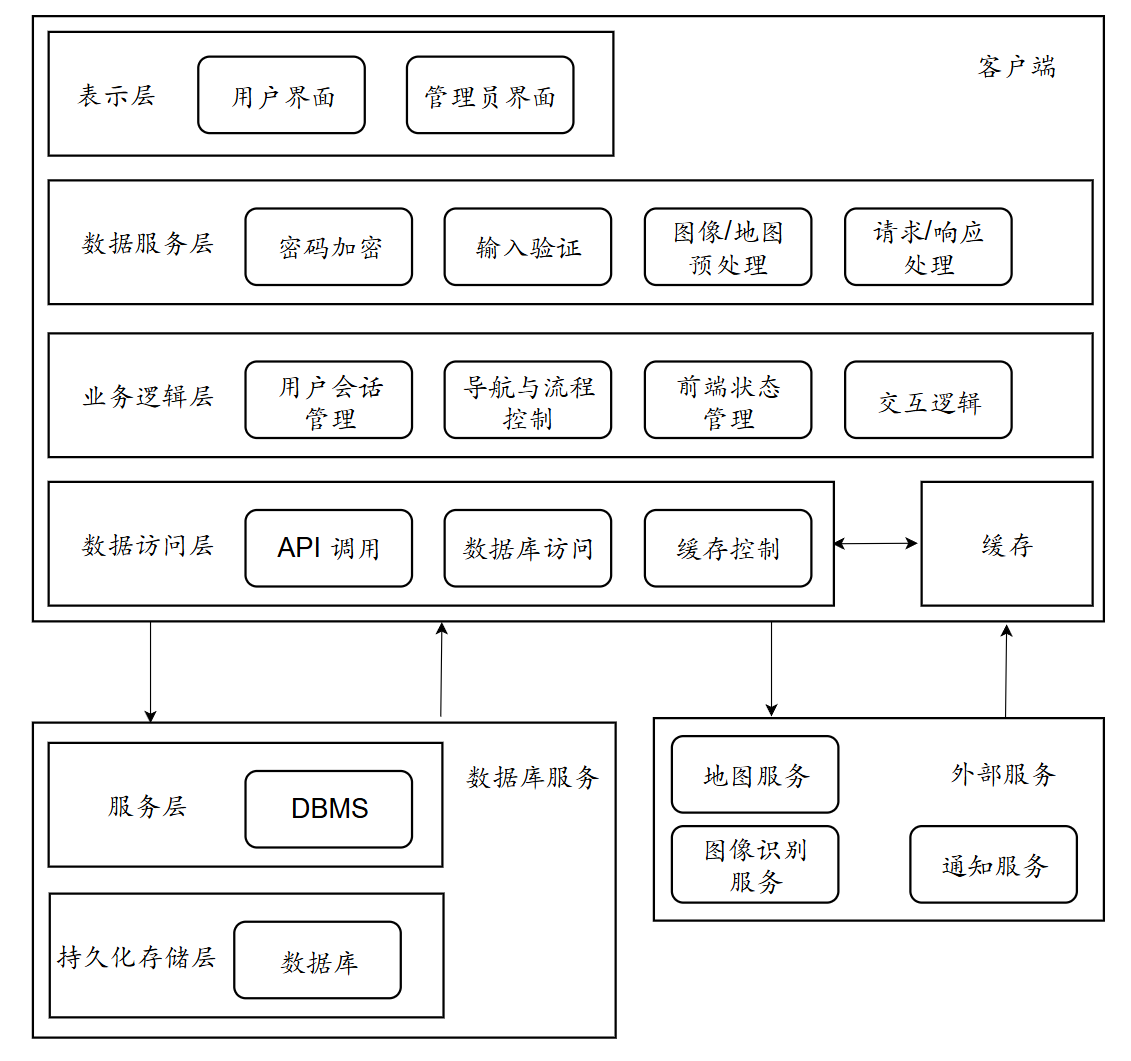
\includegraphics[width=0.9\textwidth]{figures/CA.png}
\end{figure}

\subsection{客户端}

客户端采用分层结构,分为表示层、数据服务层、业务逻辑层和数据访问层。

\vspace{0.25cm}

\textbf{表示层}:负责直接与用户交互,展示信息和接收用户输入。组件有用户界面(包含登录页、个人信息页、动物信息页、领养申请页等)和管理员界面(包括用户管理、动物信息管理和领养审核页等)两个主要部分。

\textbf{数据服务层}:提供特定的数据处理、转换或封装服务,为表示层或业务逻辑层服务。它不包含核心业务规则,更多的是数据的准备和适配。在其中包括密码加密,在用户密码发送到后端前进行客户端加密;输入数据验证,对用户在表单中输入的数据进行前端校验和初步格式化;图像和地图的预处理,能用户上传动物图片前,可能进行压缩、裁剪或格式检查,也能从地图服务获取的数据或用户输入的位置数据,转换为地图展示库所需的格式;请求/响应处理,封装对后端 API 的调用,处理响应数据的初步解析和错误处理。

\textbf{业务逻辑层}:实现客户端的核心业务流程和规则。组件有用户会话管理,处理用户登录状态;导航与流程控制,管理页面跳转逻辑,多步骤表单的流程控制;交互逻辑处理,协调外部服务和界面操作;前端状态管理,管理应用的全局或局部状态。

\textbf{数据访问层}:负责客户端与后端数据源的通信。能进行 API 调用和数据库访问,还能控制缓存。

\subsection{后端系统}

在后端系统中,我们将其简化成一个数据库服务。

\vspace{0.25cm}

\textbf{服务层}:\verb|DBMS|,如我们使用的 \verb|MySQL|。

\textbf{持久化存储层}:数据库本身,存储所有应用数据。

\subsection{外部服务}

我们的系统会依赖部分第三方服务,如地图、图像识别和通知服务。

\vspace{0.25cm}

\textbf{地图服务}:如高德地图 \verb|API| 等,用于显示地图、地理编码和位置服务。

\textbf{图像识别服务}: 第三方 \verb|AI| 服务,用于识别用户上传的动物图片。

\textbf{通知服务}:邮件推送服务,用于发送系统通知。

\section{数据库设计}

\subsection{ER 图}

\begin{figure}[H]
  \centering
  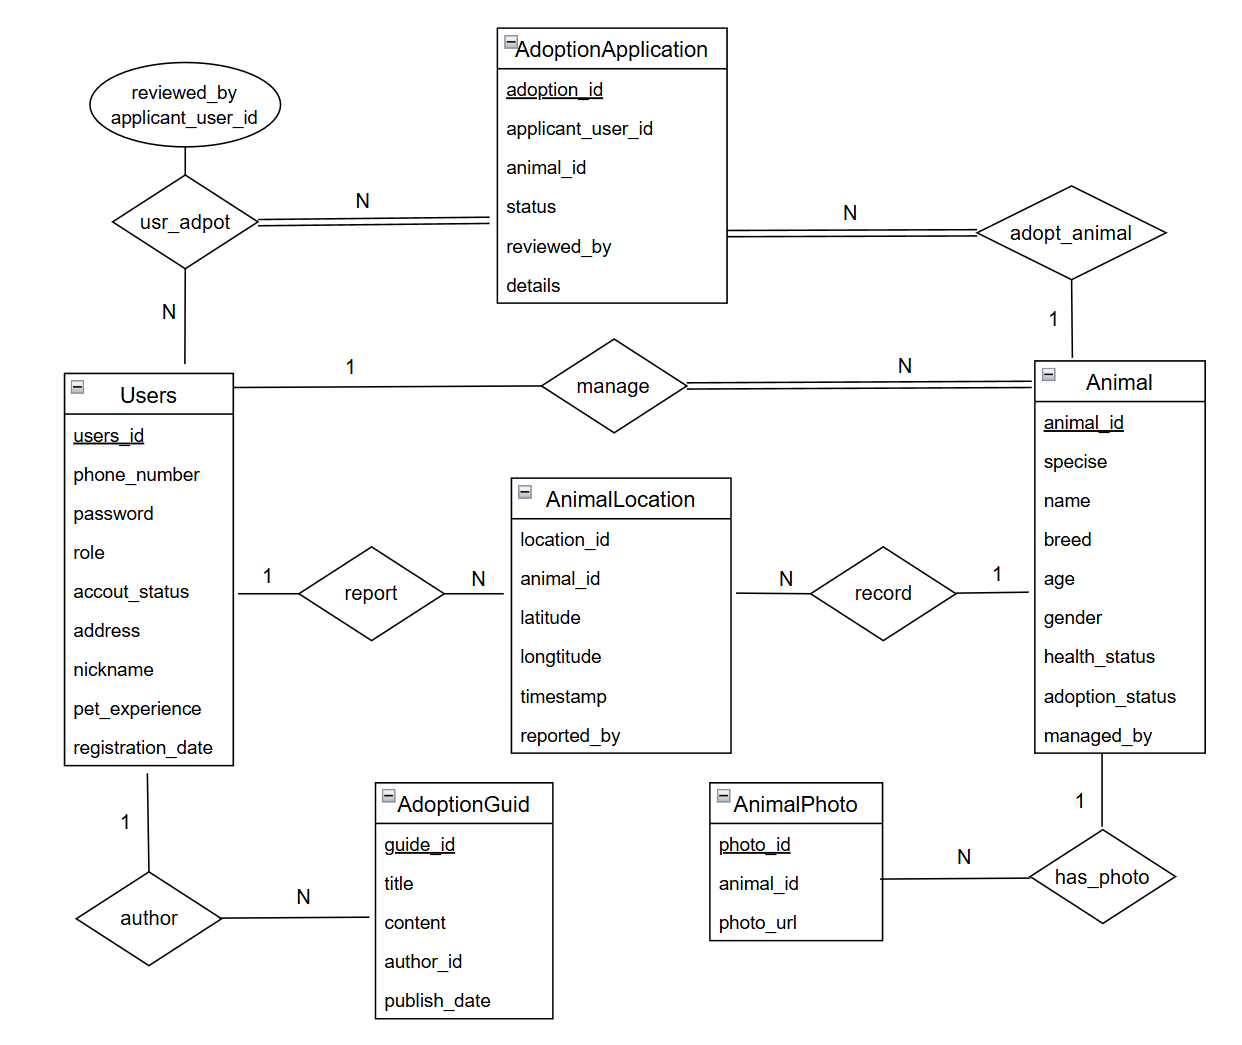
\includegraphics[width=0.9\textwidth]{figures/er.png}
\end{figure}


\subsection{逻辑结构设计}



\noindent\textbf{用户表}

主键是 \verb|users_id|,是用户唯一的标识符。

\verb|Users(users_id,phone_number,password,role,accout_status,nickname,| \\ \verb|address,pet_experience,registration_date)|


\vspace{0.25cm}

\noindent\textbf{动物表}

主键是 \verb|animal_id|,是动物唯一的标识符。外键是 \verb|managed_by|,指向用户表中的 \verb|users_id|,表示该动物由哪个用户管理。

\verb|Animals(animal_id,name,specise,breed,age,gender,health_status,| \\ \verb|adoption_status,managed_by)|


\vspace{0.25cm}

\noindent\textbf{动物照片表}

主键是 \verb|photo_id|,是照片唯一的标识符。外键是 \verb|animal_id|,指向动物表中的 \verb|animal_id|,表示该照片属于哪个动物。

\verb|AnimalPhotos(photo_id,animal_id,photo_url)|

\vspace{0.25cm}

\noindent\textbf{领养申请表}

主键是 \verb|adoption_id|,是领养申请唯一的标识符。外键有 \verb|animal_id|,指向动物表中的 \verb|animal_id|,表示该申请对应的动物;\verb|applicant_user_id|,指向用户表中的 \verb|users_id|,表示申请人;\verb|reviewed_by|,指向用户表中的 \verb|users_id|,表示审核人。

\verb|AdoptionApplications(adoption_id,animal_id,applicant_user_id,status,|\\ \verb|reviewed_by,details)|

\vspace{0.25cm}

\noindent\textbf{领养指南表}

主键是 \verb|guide_id|,是领养指南唯一的标识符。外键是 \verb|author_id|,指向用户表中的 \verb|users_id|,表示该指南的作者。

\verb|AdoptionGuides(guide_id,title,content,author_id,publish_date)|

\vspace{0.25cm}

\noindent\textbf{动物位置记录表}

主键是 \verb|location_id|,是位置记录唯一的标识符。外键有 \verb|animal_id|,指向动物表中的 \verb|animal_id|,表示该位置记录对应的动物;\verb|reported_by|,指向用户表中的 \verb|users_id|,表示报告该位置记录的用户。

\verb|AnimalLocations(location_id,animal_id,latitude,longtitude,timestamp,|\\ \verb|reported_by)|



\subsection{物理结构设计}

\noindent\textbf{用户表}


\begin{xltabular}{\linewidth}{|>{\raggedright\arraybackslash}p{4cm}|>{\raggedright\arraybackslash}p{3cm}|>{\raggedright\arraybackslash}p{1cm}|>{\raggedright\arraybackslash}p{1cm}|>{\raggedright\arraybackslash}p{5cm}|}
\hline
\textbf{字段名} & \textbf{数据类型} & \textbf{主键} & \textbf{外键} & \textbf{备注} \\ \hline
\endfirsthead

\hline
\textbf{字段名} & \textbf{数据类型} & \textbf{主键} & \textbf{外键} & \textbf{备注} \\ \hline
\endhead

\hline
\multicolumn{5}{r}{接下页} \\
\endfoot

\hline 
\endlastfoot

\verb|users_id| & \verb|int| & 是 & 否 & 用户唯一标识符,自增 \\ \hline
\verb|phone_number| & \verb|varchar(20)| & 否 & 否 & 用户手机号,用于登录,有唯一性 \\ \hline
\verb|password| & \verb|varchar(255)| & 否 & 否 & 存储用户密码的哈希值 \\ \hline
\verb|role| & \verb|varchar(20)| & 否 & 否 & 用户角色 \\ \hline
\verb|accout_status| & \verb|varchar(20)| & 否 & 否 & 账户状态\\ \hline
\verb|nickname| & \verb|varchar(50)| & 否 & 否 & 用户昵称 \\ \hline
\verb|address| & \verb|varchar(255)| & 否 & 否 & 用户地址 \\ \hline
\verb|pet_experience| & \verb|text| & 否 & 否 & 用户养宠经验描述 \\ \hline
\verb|registration_date| & \verb|timestamp| & 否 & 否 & 用户注册日期时间 \\ \hline
\end{xltabular}

\vspace{0.25cm}

\noindent\textbf{动物表}

\begin{xltabular}{\linewidth}{|>{\raggedright\arraybackslash}p{3.5cm}|>{\raggedright\arraybackslash}p{3cm}|>{\raggedright\arraybackslash}p{1cm}|>{\raggedright\arraybackslash}p{1cm}|>{\raggedright\arraybackslash}p{5cm}|}
\hline
\textbf{字段名} & \textbf{数据类型} & \textbf{主键} & \textbf{外键} & \textbf{备注} \\ \hline
\endfirsthead

\hline
\textbf{字段名} & \textbf{数据类型} & \textbf{主键} & \textbf{外键} & \textbf{备注} \\ \hline
\endhead

\hline
\multicolumn{5}{r}{接下页} \\
\endfoot

\hline 
\endlastfoot

\verb|animal_id| & \verb|int| & 是 & 否 & 动物唯一标识符, 自增 \\ \hline
\verb|name| & \verb|varchar(100)| & 否 & 否 & 动物名称 \\ \hline
\verb|specise| & \verb|varchar(50)| & 否 & 否 & 动物种类 \\ \hline
\verb|breed| & \verb|varchar(50)| & 否 & 否 & 动物具体品种 \\ \hline
\verb|age| & \verb|varchar(50)| & 否 & 否 & 动物年龄\\ \hline
\verb|gender| & \verb|varchar(10)| & 否 & 否 & 动物性别\\ \hline
\verb|health_status| & \verb|text| & 否 & 否 & 动物健康状况描述 \\ \hline
\verb|adoption_status| & \verb|varchar(20)| & 否 & 否 & 领养状态 \\ \hline
\verb|managed_by| & \verb|int| & 否 & 是 & 管理该动物的用户\\ \hline
\end{xltabular}

\vspace{0.25cm}

\noindent\textbf{动物照片表}

\begin{xltabular}{\linewidth}{|>{\raggedright\arraybackslash}p{3cm}|>{\raggedright\arraybackslash}p{3cm}|>{\raggedright\arraybackslash}p{1cm}|>{\raggedright\arraybackslash}p{1cm}|>{\raggedright\arraybackslash}p{5cm}|}
\hline
\textbf{字段名} & \textbf{数据类型} & \textbf{主键} & \textbf{外键} & \textbf{备注} \\ \hline
\endfirsthead

\hline
\textbf{字段名} & \textbf{数据类型} & \textbf{主键} & \textbf{外键} & \textbf{备注} \\ \hline
\endhead

\hline
\multicolumn{5}{r}{接下页} \\
\endfoot

\hline 
\endlastfoot

\verb|photo_id| & \verb|int| & 是 & 否 & 照片唯一标识符, 自增 \\ \hline
\verb|animal_id| & \verb|int| & 否 & 是 & 该照片所属的动物  \\ \hline
\verb|photo_url| & \verb|varchar(255)| & 否 & 否 & 照片的地址 \\ \hline
\end{xltabular}

\vspace{0.25cm}

\noindent\textbf{领养申请表}

\begin{xltabular}{\linewidth}{|>{\raggedright\arraybackslash}p{4cm}|>{\raggedright\arraybackslash}p{3cm}|>{\raggedright\arraybackslash}p{1cm}|>{\raggedright\arraybackslash}p{1cm}|>{\raggedright\arraybackslash}p{5cm}|}
\hline
\textbf{字段名} & \textbf{数据类型} & \textbf{主键} & \textbf{外键} & \textbf{备注} \\ \hline
\endfirsthead

\hline
\textbf{字段名} & \textbf{数据类型} & \textbf{主键} & \textbf{外键} & \textbf{备注} \\ \hline
\endhead

\hline
\multicolumn{5}{r}{接下页} \\
\endfoot

\hline 
\endlastfoot

\verb|adoption_id| & \verb|int| & 是 & 否 & 领养申请唯一标识符, 自增 \\ \hline
\verb|animal_id| & \verb|int| & 否 & 是 & 申请领养的动物 \\ \hline
\verb|applicant_user_id| & \verb|int| & 否 & 是 & 提交申请的用户 \\ \hline
\verb|status| & \verb|varchar(20)| & 否 & 否 & 申请状态\\ \hline
\verb|reviewed_by| & \verb|int| & 否 & 是 & 审核该申请的管理员用户\\ \hline
\verb|details| & \verb|text| & 否 & 否 & 申请相关的详细信息\\ \hline
\end{xltabular}

\vspace{0.25cm}

\noindent\textbf{领养指南表}

\begin{xltabular}{\linewidth}{|>{\raggedright\arraybackslash}p{3cm}|>{\raggedright\arraybackslash}p{3cm}|>{\raggedright\arraybackslash}p{1cm}|>{\raggedright\arraybackslash}p{1cm}|>{\raggedright\arraybackslash}p{5cm}|}
\hline
\textbf{字段名} & \textbf{数据类型} & \textbf{主键} & \textbf{外键} & \textbf{备注} \\ \hline
\endfirsthead

\hline
\textbf{字段名} & \textbf{数据类型} & \textbf{主键} & \textbf{外键} & \textbf{备注} \\ \hline
\endhead

\hline
\multicolumn{5}{r}{接下页} \\
\endfoot

\hline 
\endlastfoot

\verb|guide_id| & \verb|int| & 是 & 否 & 领养指南唯一标识符, 自增 \\ \hline
\verb|title| & \verb|varchar(255)| & 否 & 否 & 指南标题 \\ \hline
\verb|content| & \verb|text| & 否 & 否 & 指南详细内容 \\ \hline
\verb|author_id| & \verb|int| & 否 & 是 & 指南作者的用户\\ \hline
\verb|publish_date| & \verb|timestamp| & 否 & 否 & 指南发布日期时间 \\ \hline
\end{xltabular}

\vspace{0.25cm}

\noindent\textbf{动物位置记录表}

\begin{xltabular}{\linewidth}{|>{\raggedright\arraybackslash}p{3cm}|>{\raggedright\arraybackslash}p{3cm}|>{\raggedright\arraybackslash}p{1cm}|>{\raggedright\arraybackslash}p{1cm}|>{\raggedright\arraybackslash}p{5cm}|}
\hline
\textbf{字段名} & \textbf{数据类型} & \textbf{主键} & \textbf{外键} & \textbf{备注} \\ \hline
\endfirsthead

\hline
\textbf{字段名} & \textbf{数据类型} & \textbf{主键} & \textbf{外键} & \textbf{备注} \\ \hline
\endhead

\hline
\multicolumn{5}{r}{接下页} \\
\endfoot

\hline 
\endlastfoot

\verb|location_id| & \verb|int| & 是 & 否 & 位置记录唯一标识符, 自增 \\ \hline
\verb|animal_id| & \verb|int| & 否 & 是 & 该位置记录对应的动物\\ \hline
\verb|latitude| & \verb|decimal(9,6)| & 否 & 否 & 地理纬度 \\ \hline
\verb|longtitude| & \verb|decimal(9,6)| & 否 & 否 & 地理经度 \\ \hline
\verb|timestamp| & \verb|timestamp| & 否 & 否 & 位置记录的时间戳 \\ \hline
\verb|reported_by| & \verb|int| & 否 & 是 & 报告该位置记录的用户\\ \hline
\end{xltabular}

\section{关键过程}

\subsection{用户注册登录过程}

\subsubsection{用户注册过程}

触发条件:用户在未登录的情况下,点击界面的注册选项。主要步骤如下:

\begin{enumerate}[topsep=2pt, partopsep=0pt]
  \item 系统导航至用户注册界面
  \item 用户在注册表单中输入必要信息,如手机号、密码、确认密码
  \item 进行前端校验,确保输入信息的有效性
  \item 提交注册请求,客户端将注册信息封装,发送后端
  \item 后端进行处理,判断手机号是否被注册登数据校验,再将密码进行安全的处理,最后数据持久化
  \item 后端向客户端返回注册结果,成功返回消息,引导至登录界面
\end{enumerate}

\subsubsection{用户登录过程}

触发条件:用户在未登录的情况下,点击界面的登录选项。主要步骤如下:

\begin{enumerate}[topsep=2pt, partopsep=0pt]
  \item 系统导航至用户登录界面
  \item 用户在登录表单中输入必要信息,如手机号、密码
  \item 进行前端校验,确保输入信息的有效性
  \item 提交登录请求,客户端将登录信息封装,发送后端
  \item 后端进行处理,进行用户查找、密码校验、更新登录状态等
  \item 后端向客户端返回登录结果,引导至个人首页
\end{enumerate}

\subsection{动物信息管理过程}

\subsubsection{管理员编辑动物信息过程}

触发条件:管理员在后台管理界面选择创建新动物信息或编辑现有动物信息。主要步骤如下:

\begin{enumerate}[topsep=2pt, partopsep=0pt]
  \item 系统展示一个空的动物信息表单,或根据指定的动物加载现有数据信息
  \item 管理员填写或修改动物的各项信息
  \item 进行前端校验,对必填项、数据格式等进行校验
  \item 提交创建、修改申请,客户端将完整的动物信息封装,发送后端
  \item 后端进行处理,验证权限和数据校验,再进行数据创建与更新,记录操作日志
  \item 服务端返回操作结果
\end{enumerate}

\subsubsection{普通用户提交新动物信息过程}

与管理员创建动物信息过程类似,但是触发者为普通用户。过程有以下区别:

\begin{enumerate}[topsep=2pt, partopsep=0pt]
  \item 后端的处理不会直接修改和更新动物信息,而是先临时保存,待管理员进行审核编辑
  \item 管理员审核动物信息,批准和修改后,才会将其正式添加到系统中
\end{enumerate}

\subsubsection{用户查看动物信息过程}

触发条件:用户在动物列表页点击某个动物,或通过搜索/识图结果访问动物详情。主要步骤如下:

\begin{enumerate}[topsep=2pt, partopsep=0pt]
  \item 系统展示动物信息,由用户自由点击查看
  \item 客户端根据用户点击或搜索结果的动物 \verb|ID|,向后端请求动物信息
  \item 后端进行处理,查询动物信息表,返回动物的详细信息
  \item 客户端接收数据,展示动物的详细信息
\end{enumerate}

\subsection{领养申请与审批过程}

\subsubsection{用户提交领养申请过程}

触发条件:用户在动物详情页点击申请领养按钮。主要步骤如下:

\begin{enumerate}[topsep=2pt, partopsep=0pt]
  \item 系统导航至该动物的领养申请表单页面,预填部分用户信息
  \item 用户根据提示填写领养申请的详细信息
  \item 进行前端校验,确保输入信息的有效性
  \item 提交申请,客户端将申请信息封装,发送后端
  \item 后端进行处理,验证用户身份,检查动物是否可领养,记录申请信息,再通知管理员进行审核
  \item 后端向客户端返回申请结果,引导用户查看申请状态
\end{enumerate}

\subsubsection{管理员审核领养申请过程}

触发条件:管理员在后台管理界面查看待审核的领养申请。主要步骤如下:

\begin{enumerate}[topsep=2pt, partopsep=0pt]
  \item 系统提示待审核的领养申请列表,管理员选择某个申请进行审核
  \item 系统展示该申请的详细信息
  \item 管理员查看申请信息,决定是否批准或拒绝
  \item 提交审批结果,客户端将审核结果封装,发送后端
  \item 后端进行处理,验证权限,更新申请状态,记录操作日志
  \item 服务端向用户返回申请结果
\end{enumerate}

\subsection{动物地图定位过程}

\subsubsection{用户查看动物地图过程}

触发条件:管理员访问系统的动物地图功能模块。主要步骤如下:

\begin{enumerate}[topsep=2pt, partopsep=0pt]
  \item 客户端向后端 \verb|API| 请求在特定区域内或所有动物的位置数据
  \item 后端从动物位置表查询最新的、有效的动物位置记录
  \item 后端将动物的地理坐标列表返回给客户端
  \item 前端展示,客户端初始化地图组件,将从后端获取的位置渲染为标记点,允许用户进行地图交互和查看动物信息
\end{enumerate}

\subsubsection{用户更新动物位置过程}

触发条件:用户在动物详情页点击更新位置按钮。主要步骤如下:

\begin{enumerate}[topsep=2pt, partopsep=0pt]
  \item 用户选择点击更新某个具体动物的位置,系统导航至该动物的更新位置表单页面
  \item 用户在地图上通过手动标点、设备 \verb||GPS| 定位或输入地址等方式确定动物位置
  \item 进行前端校验,判断位置信息是否有效
  \item 客户端将位置信息发送至后端
  \item 后端进行数据校验,通知管理员进行审核,待审核后更新主表位置信息,进行数据持久化
  \item 后端返回操作结果
\end{enumerate}

\subsection{动物识图搜索过程}

触发条件:用户在系统中选择使用动物识图功能。主要步骤如下:

\begin{enumerate}[topsep=2pt, partopsep=0pt]
  \item 用户通过界面提供的入口,拍摄一张动物照片或从设备相册中选择一张图片上传
  \item 客户端可能对图片进行预处理
  \item 客户端将图片文件上传至后端服务器的特定接口
  \item 后端将图片转发给第三方图像识别服务 \verb|API|
  \item 图像识别服务返回识别结果
  \item 后端根据识别出的动物特征,查询动物信息表,返回匹配的动物列表
  \item 后端将综合的识别结果返回给客户端
  \item 客户端向用户展示识别出的动物信息,并列出系统内找到的相似动物的链接或简要信息
\end{enumerate}

\subsection{UI 数据处理与交互过程}

此过程概括了用户界面层在接受用户输入,展示数据以及与用户交互时的通用处理逻辑。关键方面如下:

\begin{itemize}[topsep=2pt, partopsep=0pt]
  \item 表单处理与验证:客户端对所有用户输入的表单数据进行即时校验,提供友好的错误提示
  \item 数据展示与渲染:从后端获取的数据需要有效地进行渲染和展示
  \item 用户反馈与状态管理:对用户的交互操作,进行即时反馈
  \item 封装请求和处理错误:统一封装对后端的请求,需要有响应与处理各种错误情况
\end{itemize}

\subsection{数据访问与持久化过程}

此过程概括了后端应用服务器在与数据库进行交互以实现数据增删改查时的通用逻辑。关键方面如下:

\begin{itemize}[topsep=2pt, partopsep=0pt]
  \item 进行数据库连接,获取和释放数据库连接
  \item 对事物管理时,需要保证原子性的操作确保数据一致性
  \item 进行数据校验和转换
  \item 记录数据库的操作处理或错误日志
\end{itemize}

\subsection{与外部服务的交互过程}

此过程概括了系统与第三方服务(如地图服务、图像识别服务)进行交互的通用模式。关键方面如下:

\begin{itemize}[topsep=2pt, partopsep=0pt]
  \item 安全地存储和使用调用第三方 \verb|API| 所需的密钥或凭证
  \item 处理格式、参数、头部信息对应的请求构建与发送
  \item 能够解析第三方服务返回的数据
  \item 将从第三方服务获取的数据转换为系统内部所需的格式
\end{itemize}


\section{界面}

\subsection{用户端界面}

\subsubsection{登录注册界面}

\begin{figure}[H]
  \centering
  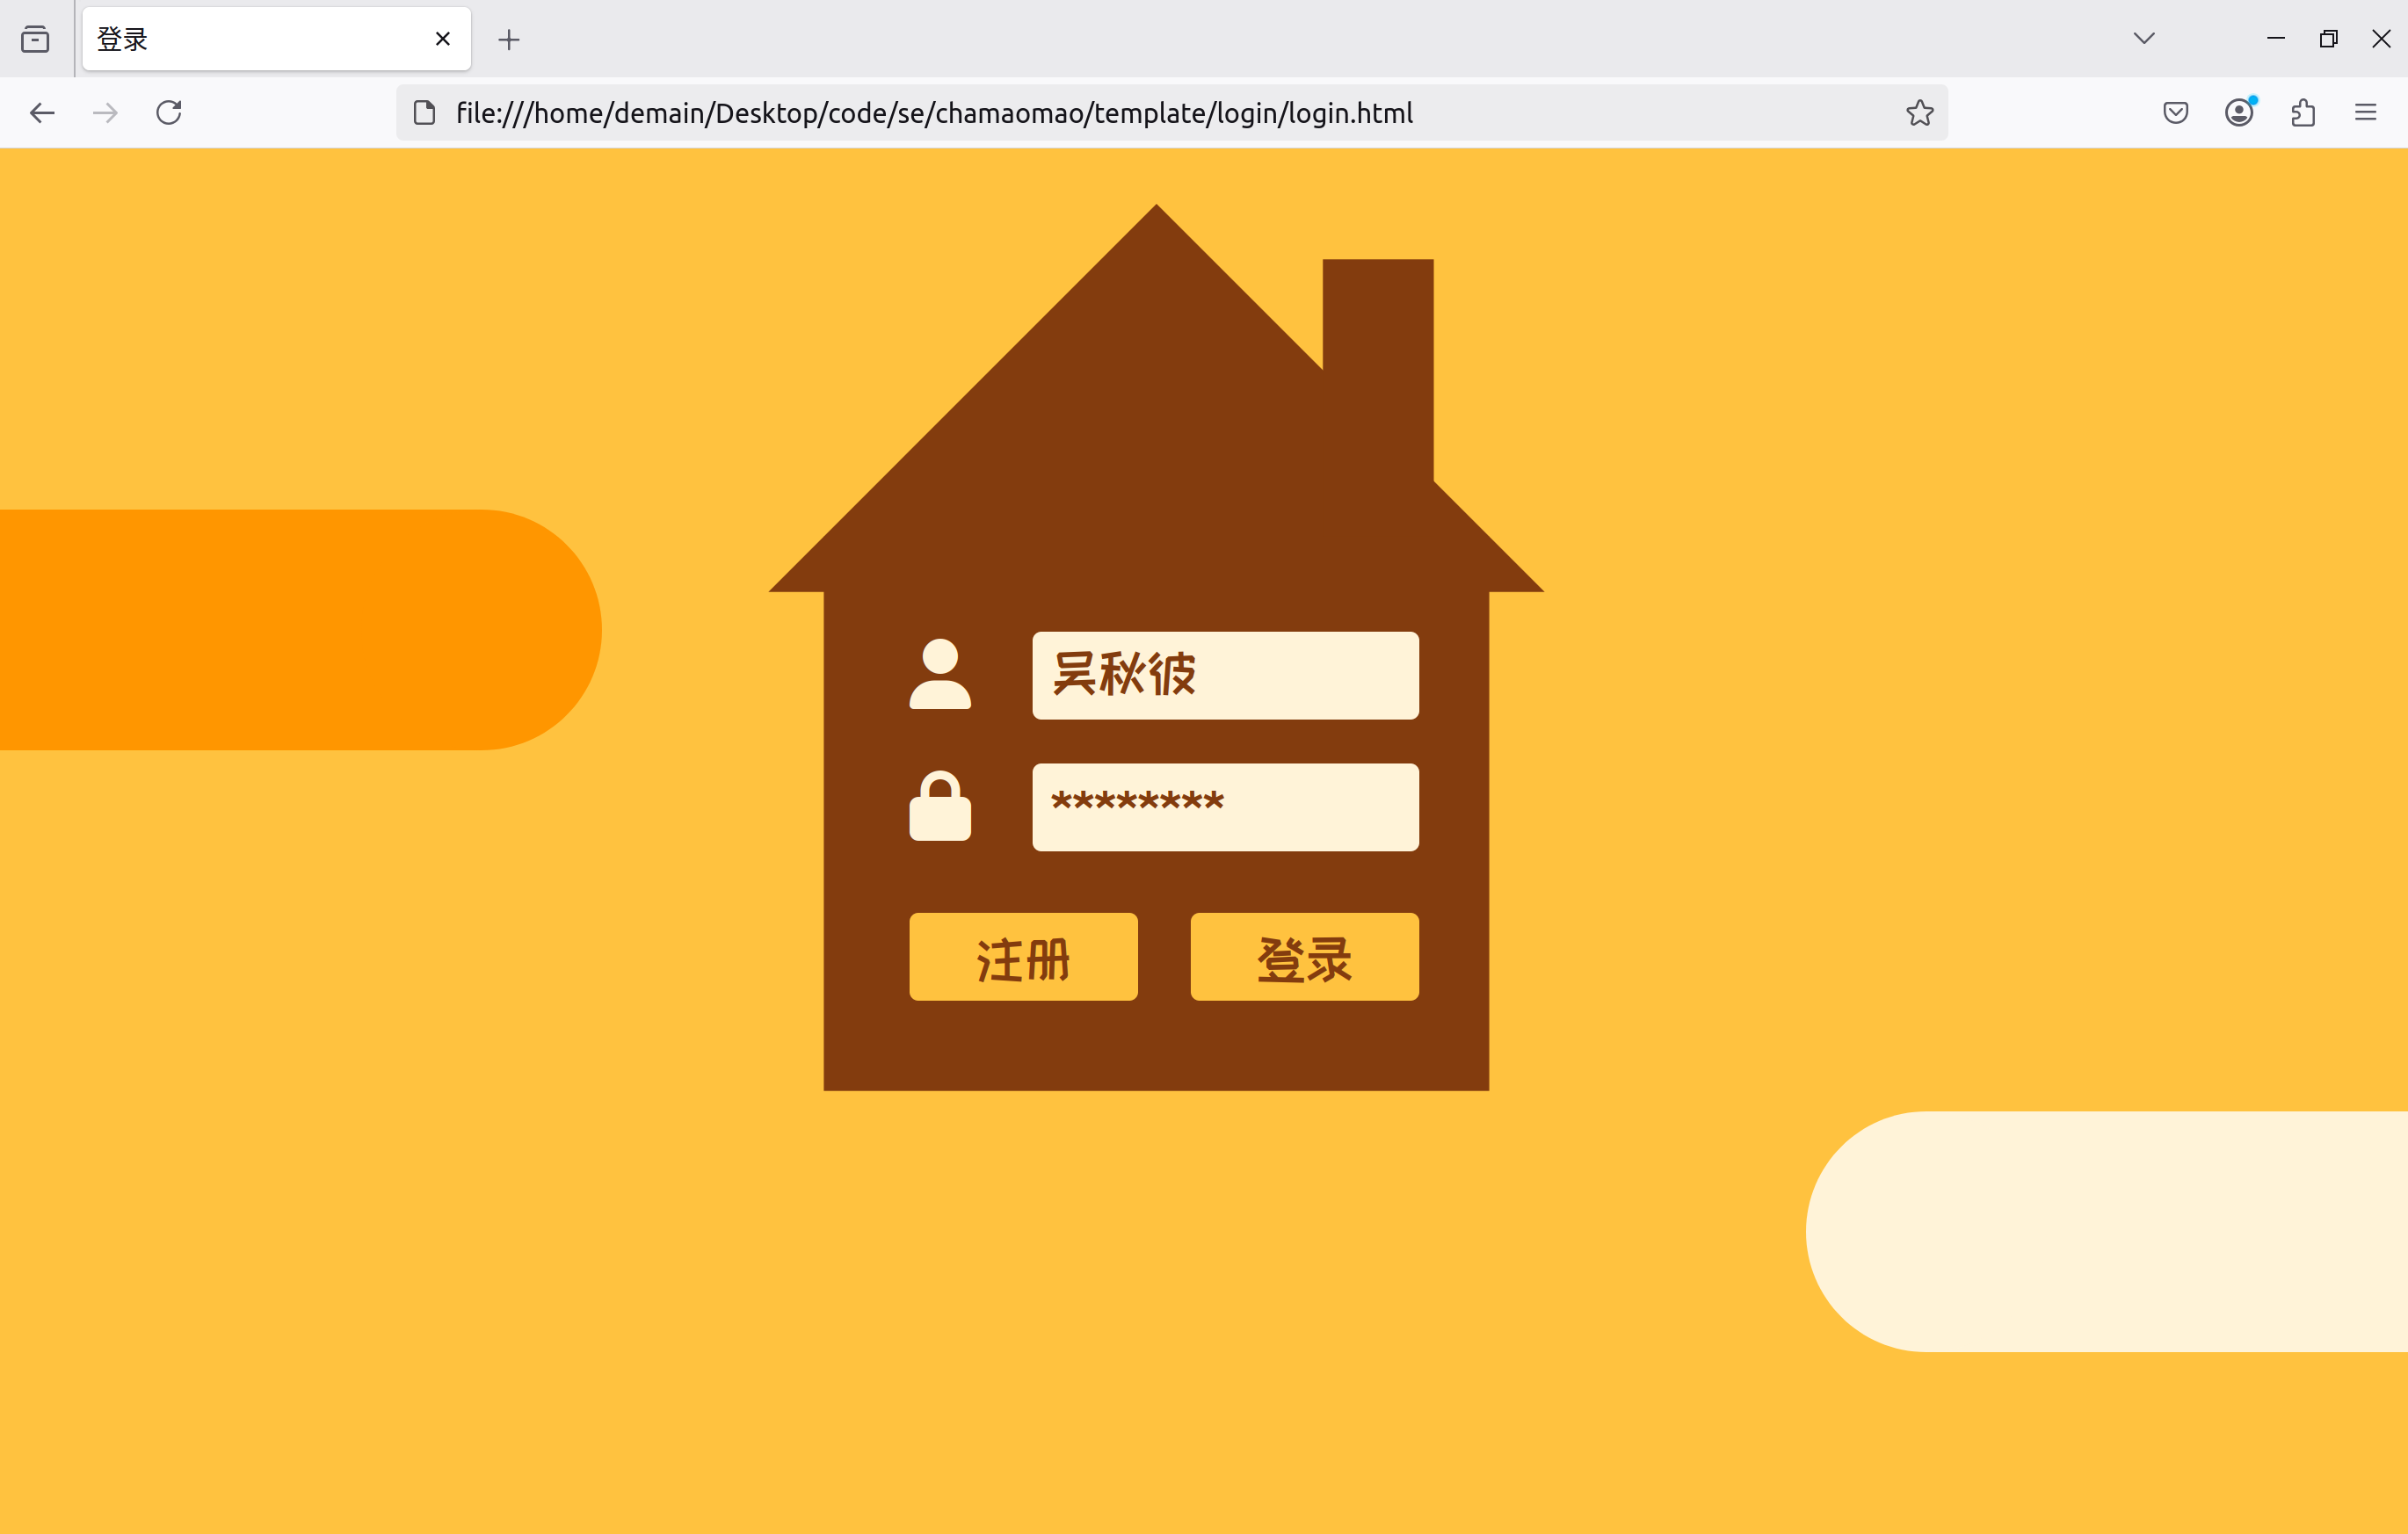
\includegraphics[width=0.9\textwidth]{figures/UserLogin.png}
\end{figure}

\subsubsection{个人信息界面}

\begin{figure}[H]
  \centering
  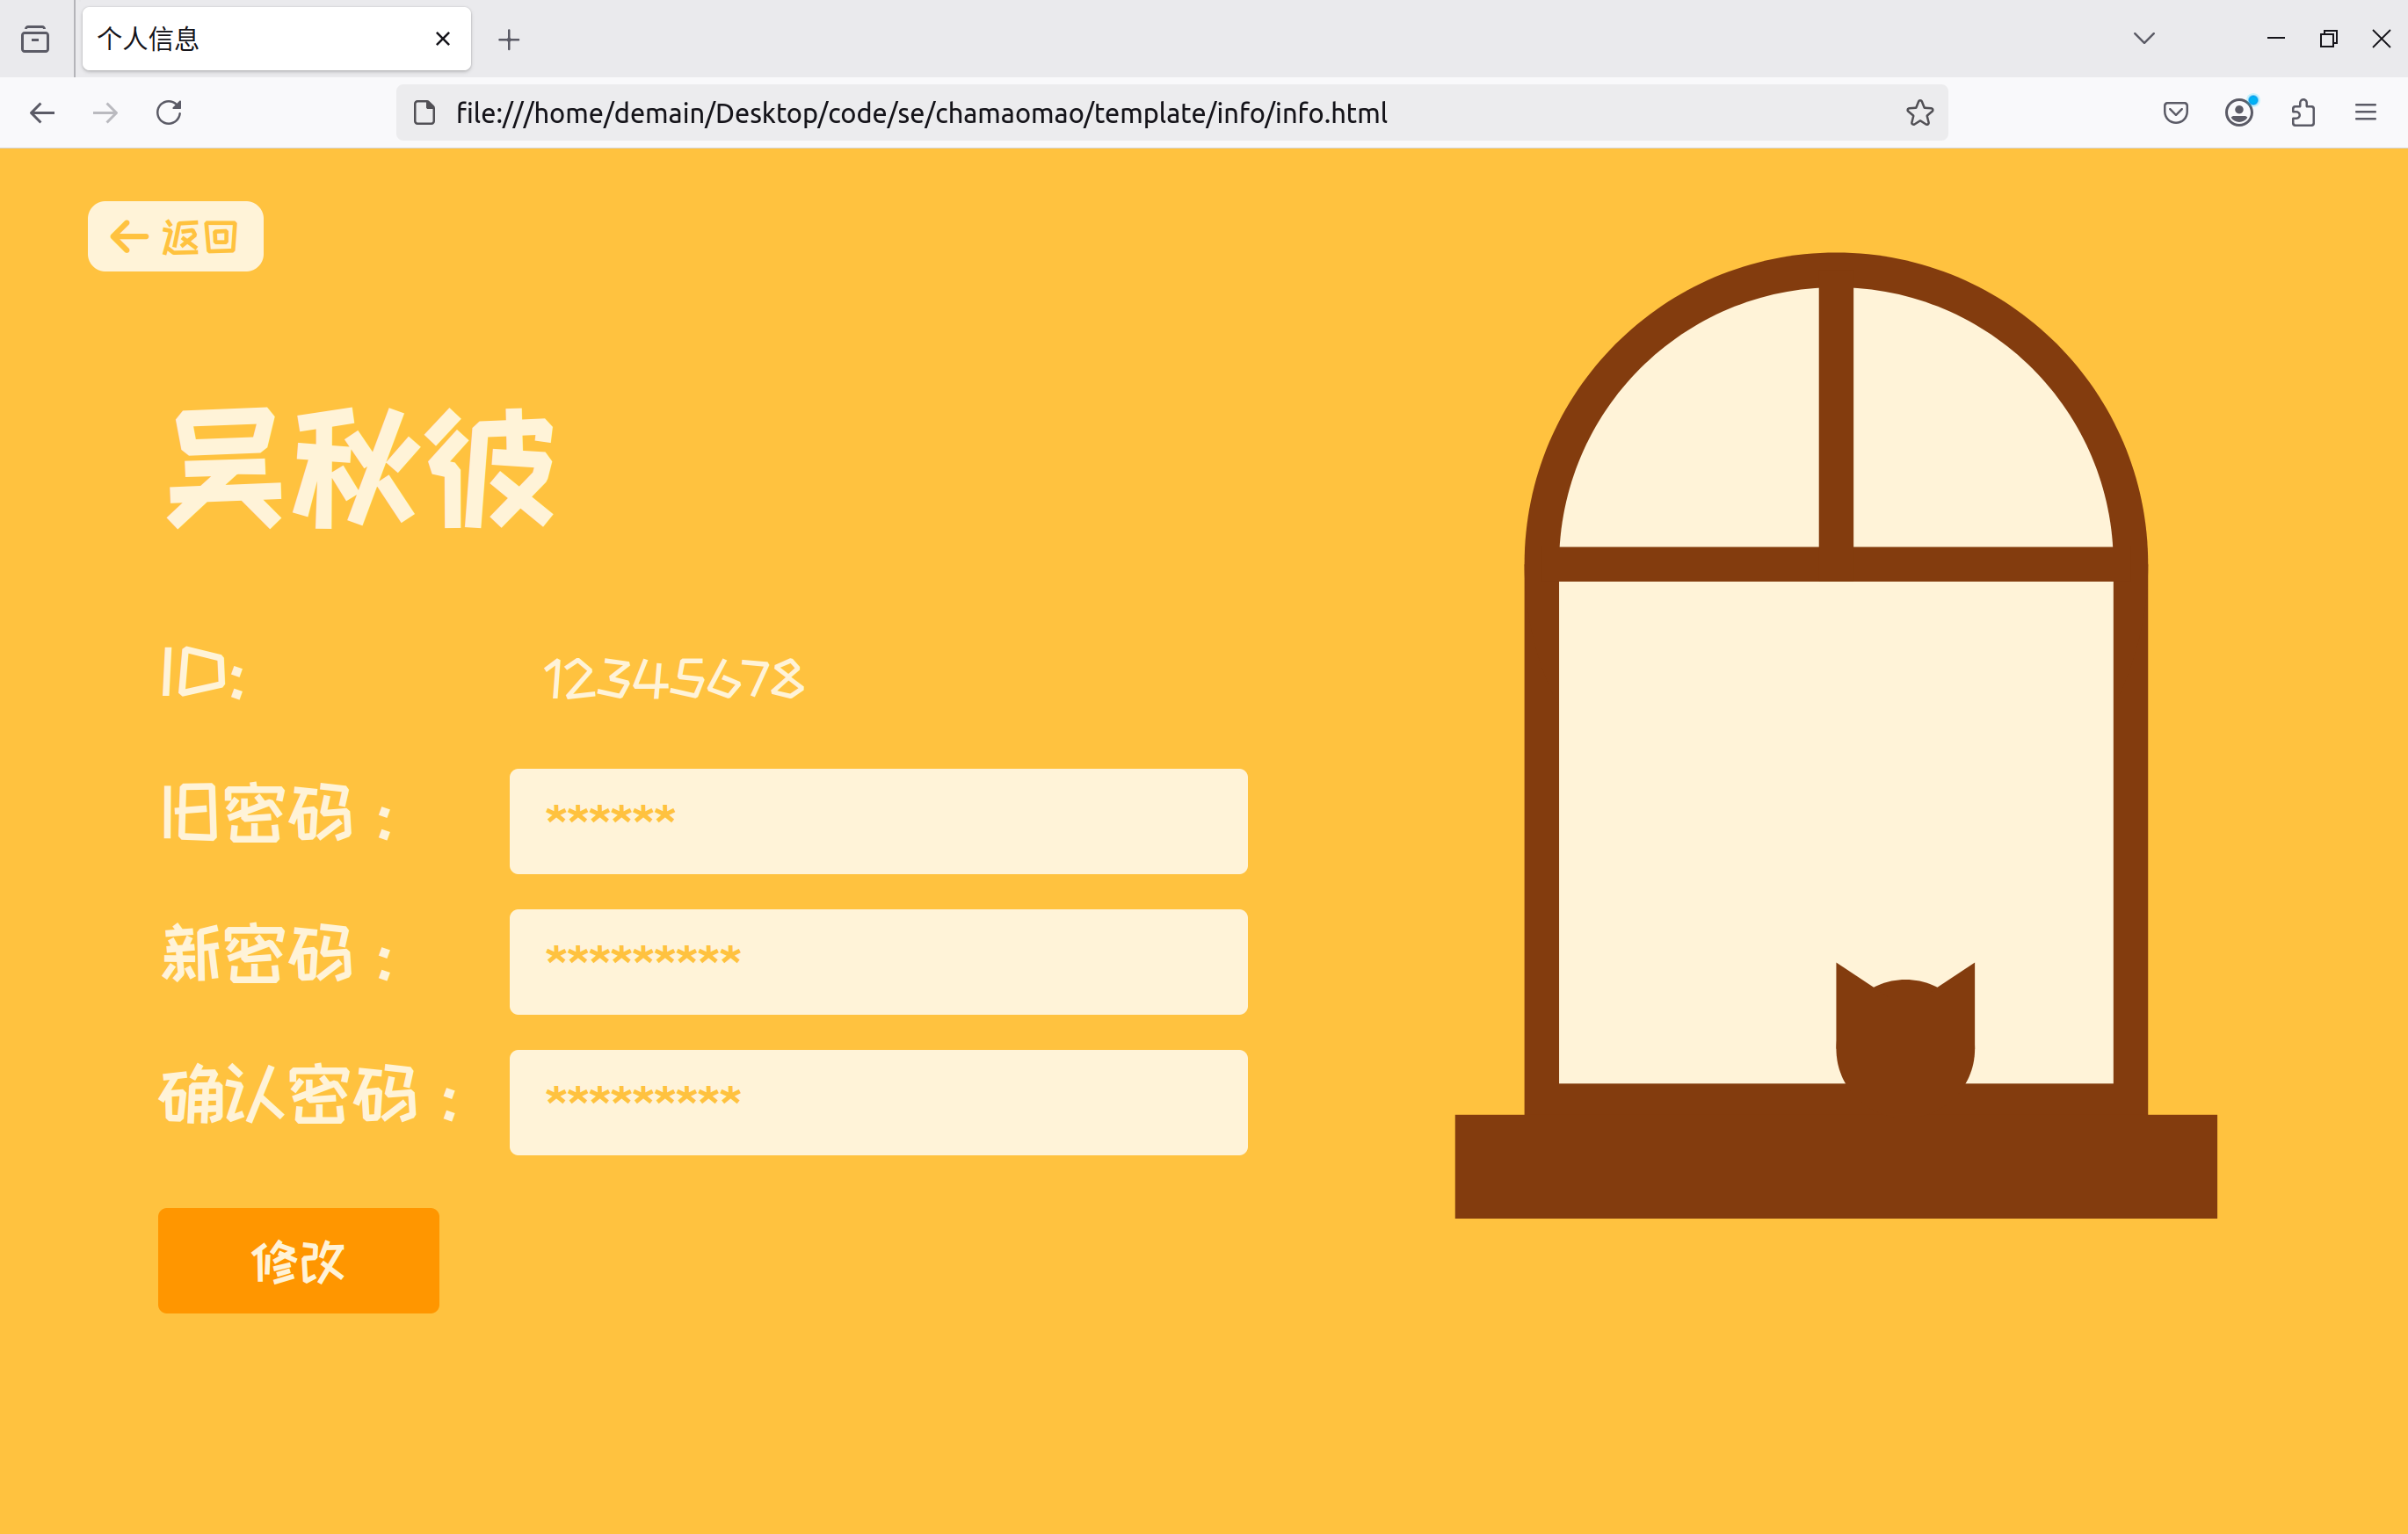
\includegraphics[width=0.9\textwidth]{figures/UserInfo.png}
\end{figure}

\subsubsection{动物信息筛选界面}

\begin{figure}[H]
  \centering
  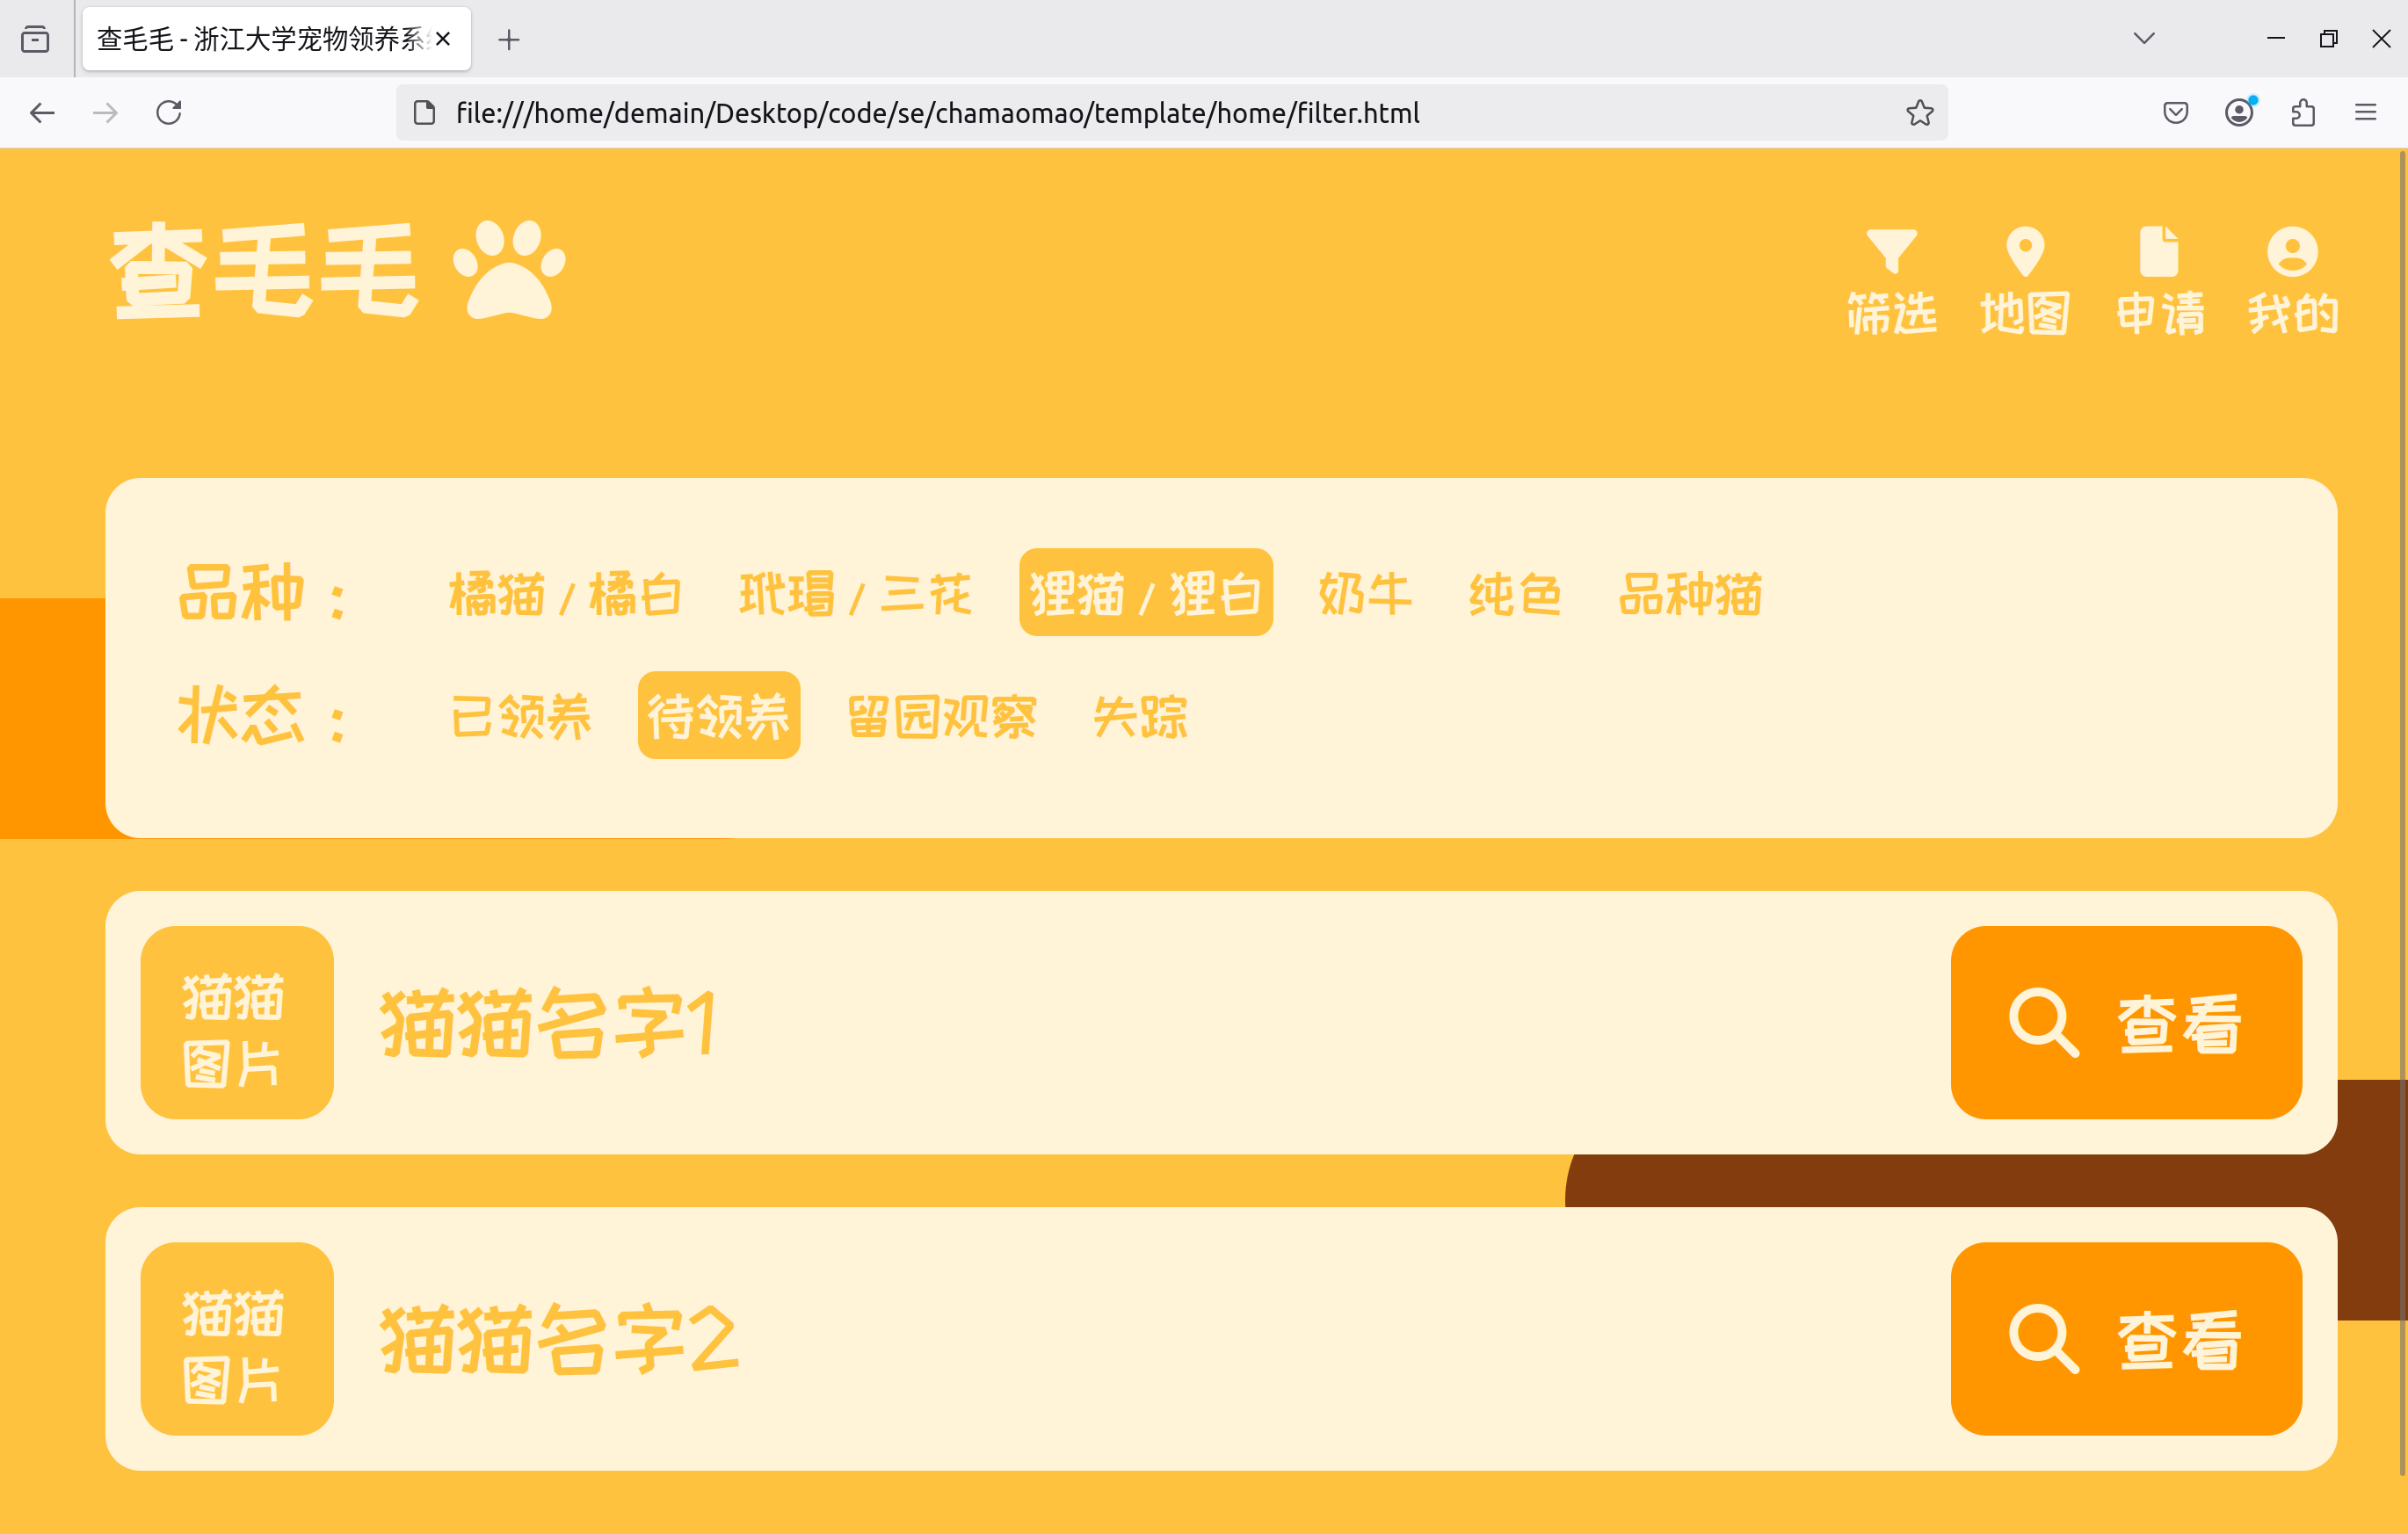
\includegraphics[width=0.9\textwidth]{figures/AnimalInfo1.png}
\end{figure}

\subsubsection{动物信息浏览界面}

\begin{figure}[H]
  \centering
  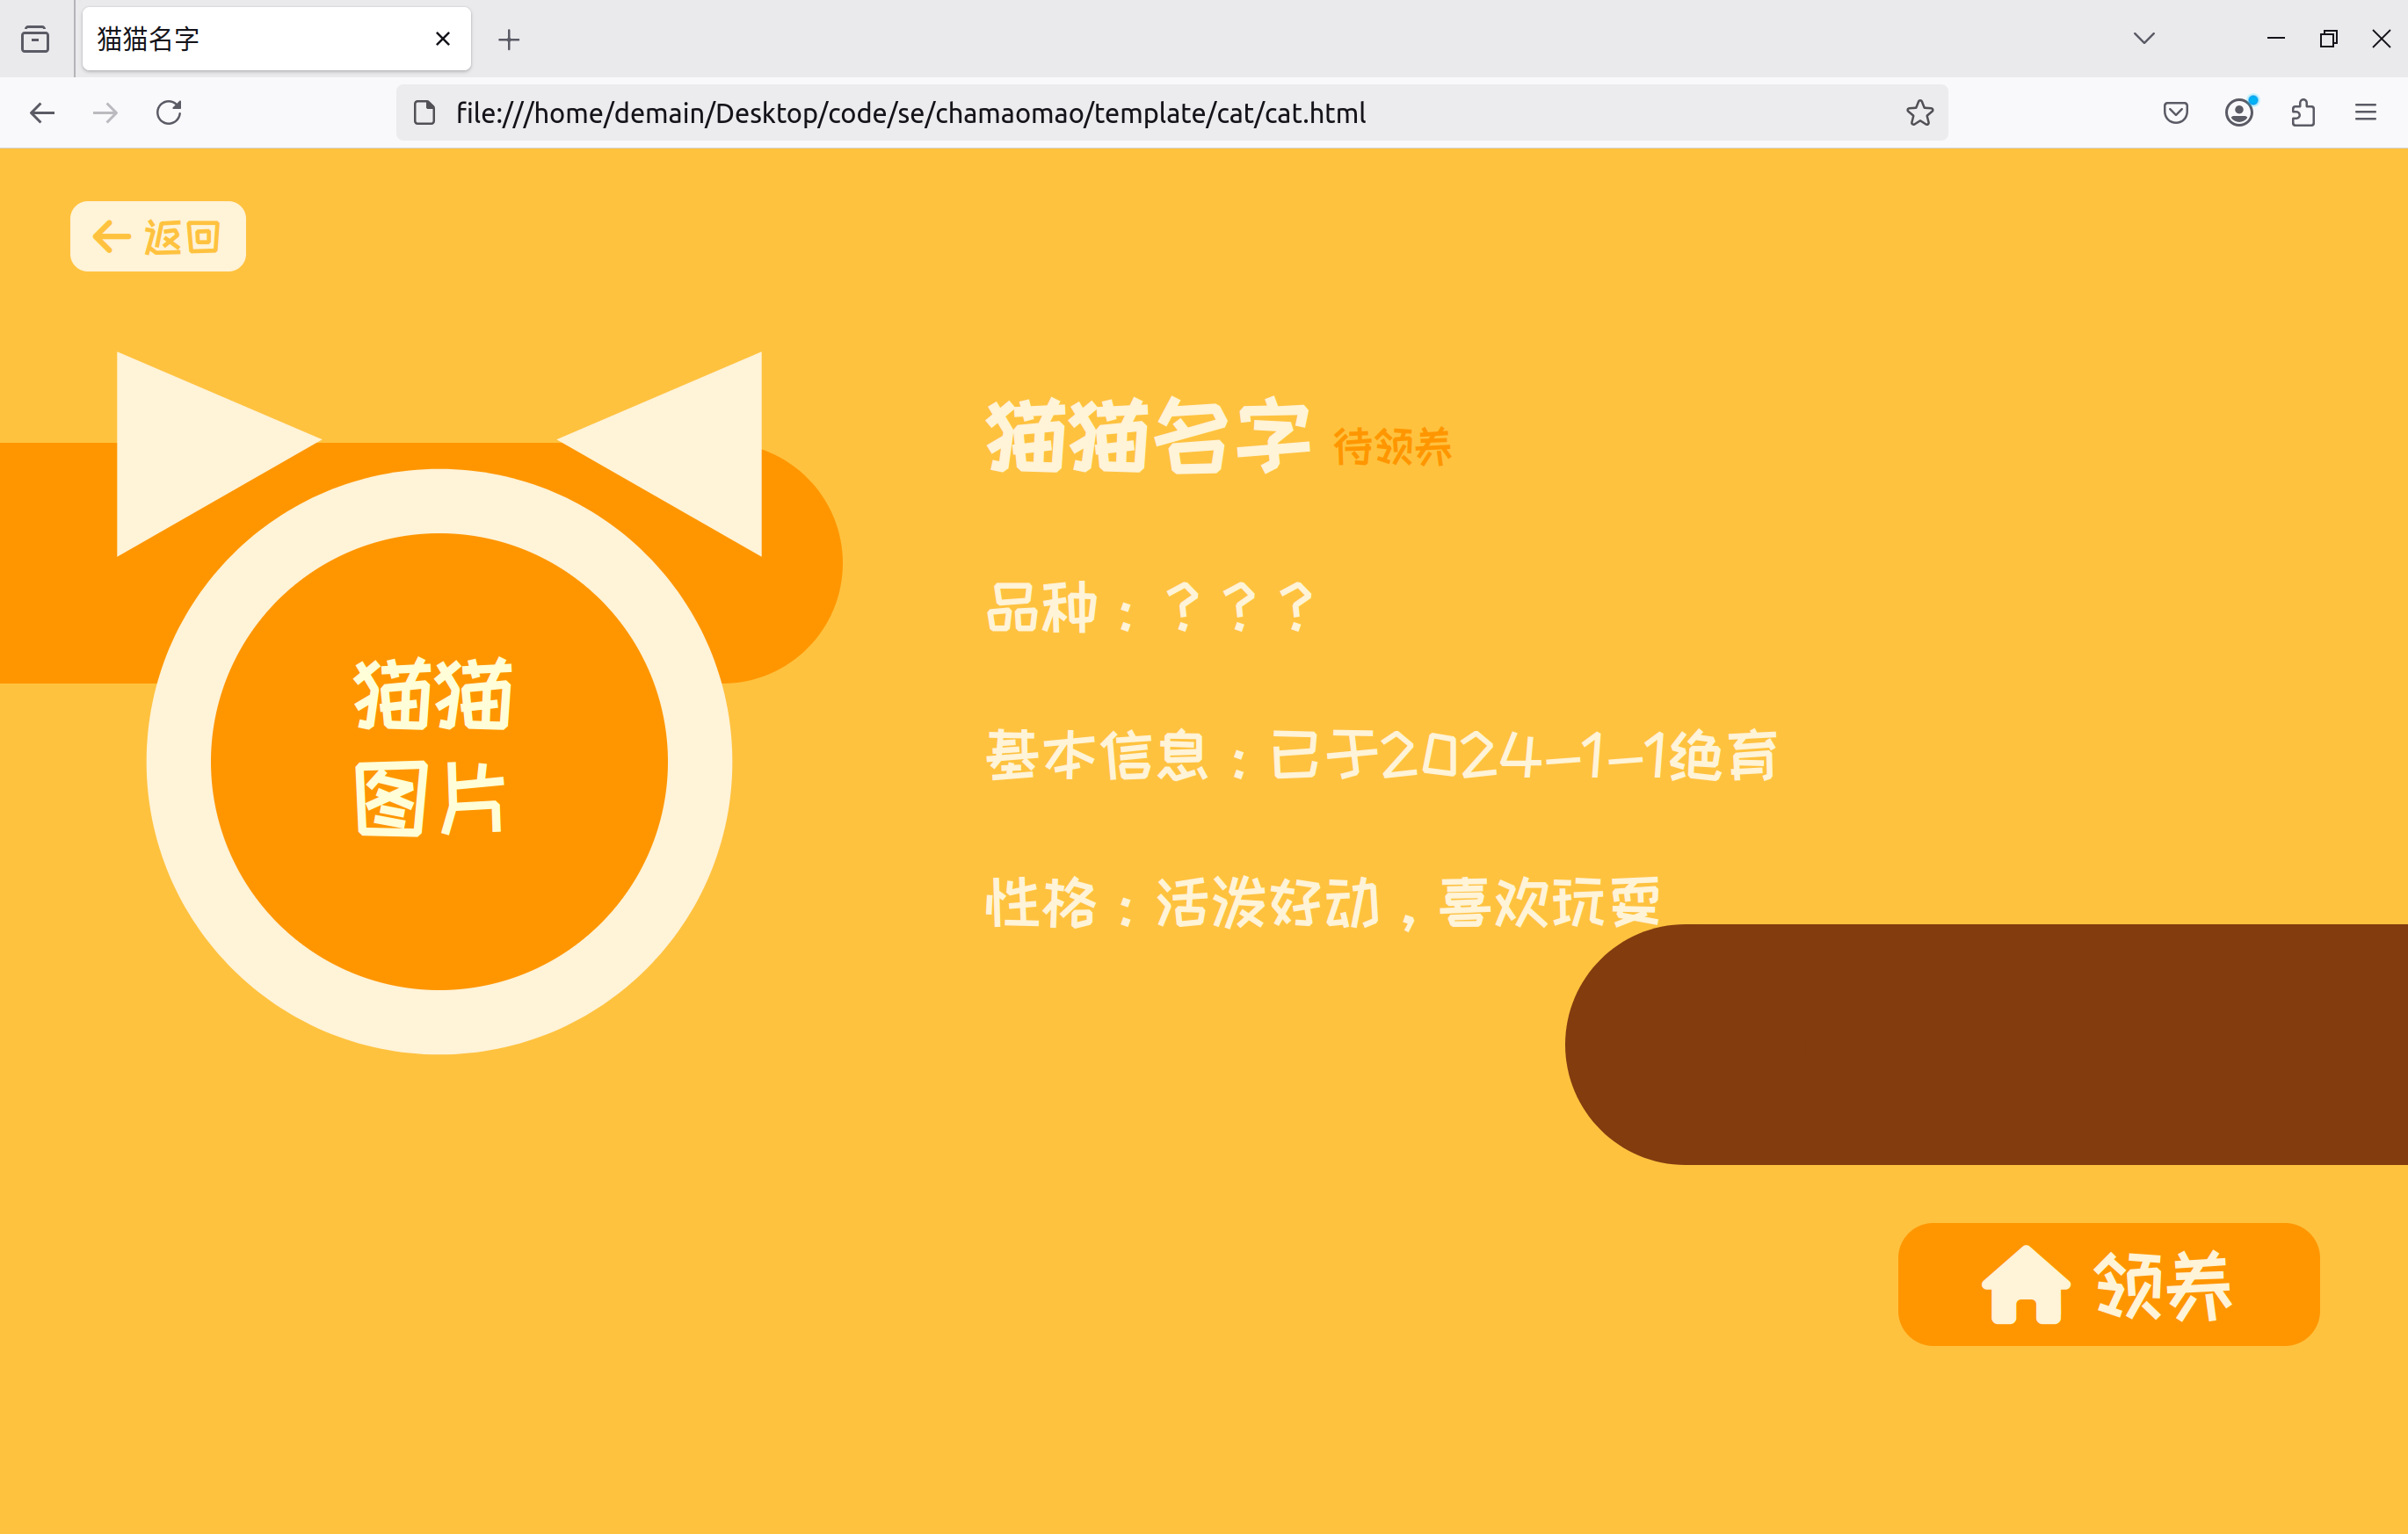
\includegraphics[width=0.9\textwidth]{figures/AnimalInfo2.png}
\end{figure}

\subsubsection{领养申请界面}

\begin{figure}[H]
  \centering
  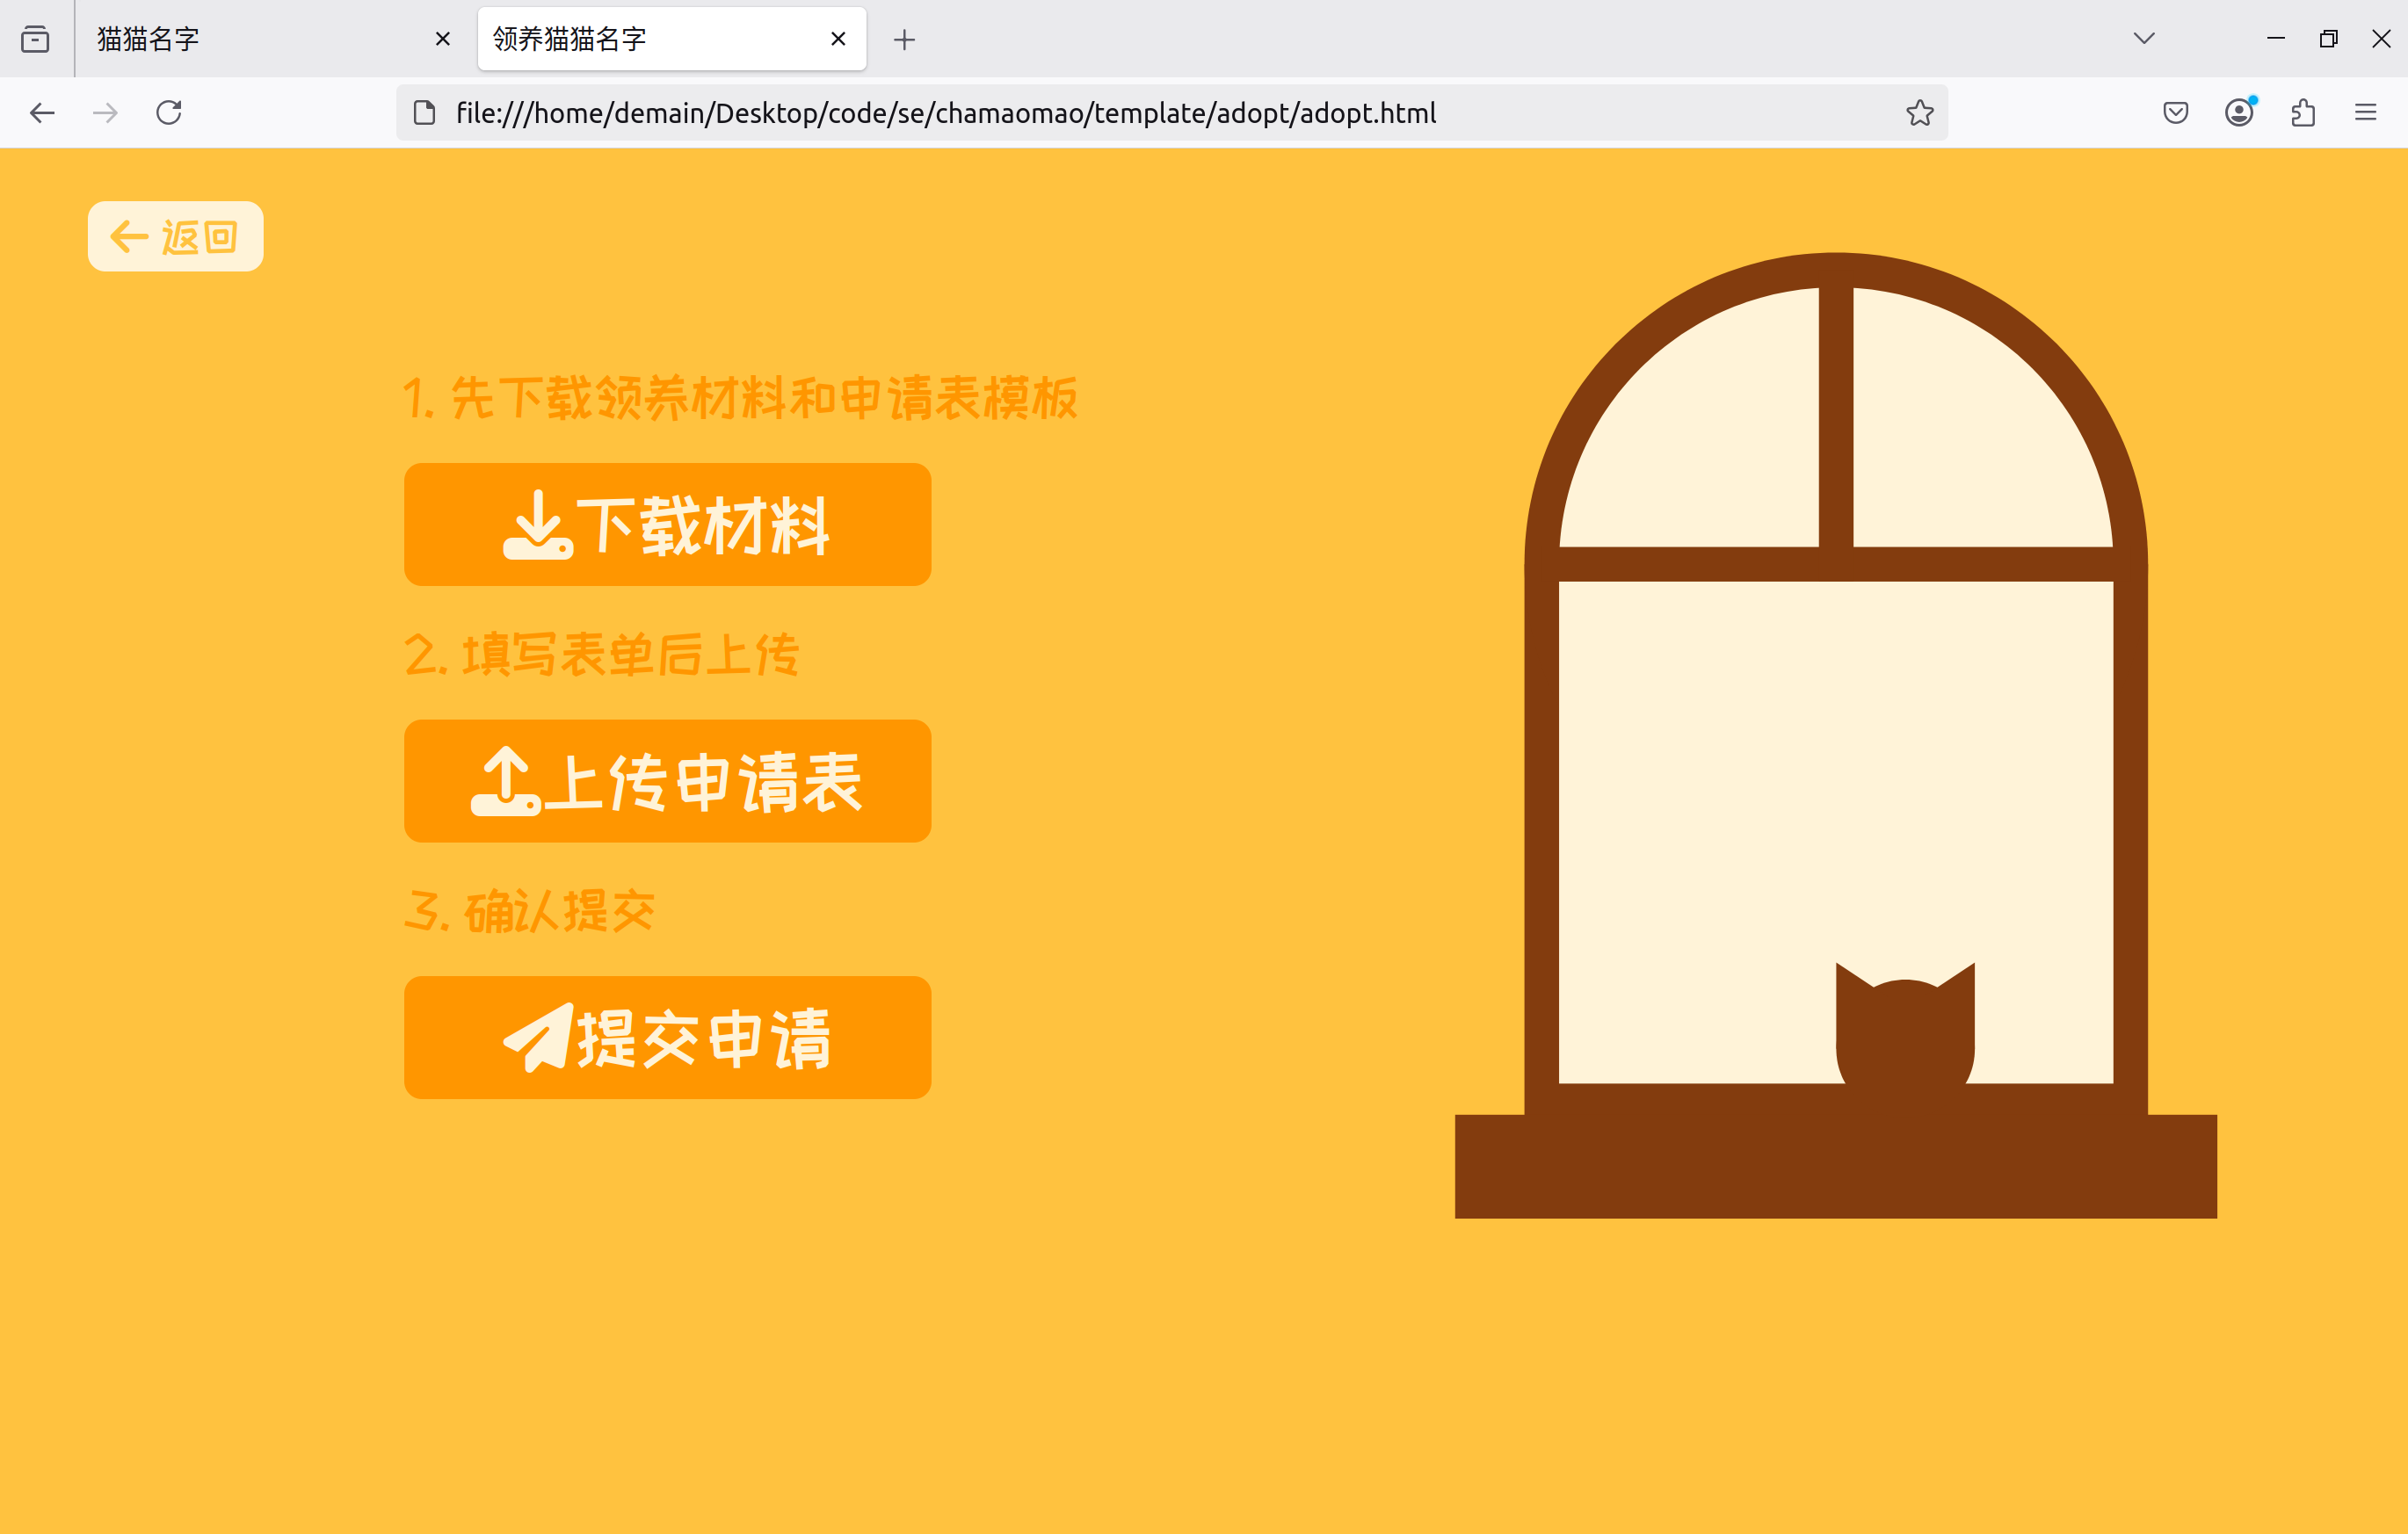
\includegraphics[width=0.9\textwidth]{figures/AdoptionApply5.png}
\end{figure}

\begin{figure}[H]
  \centering
  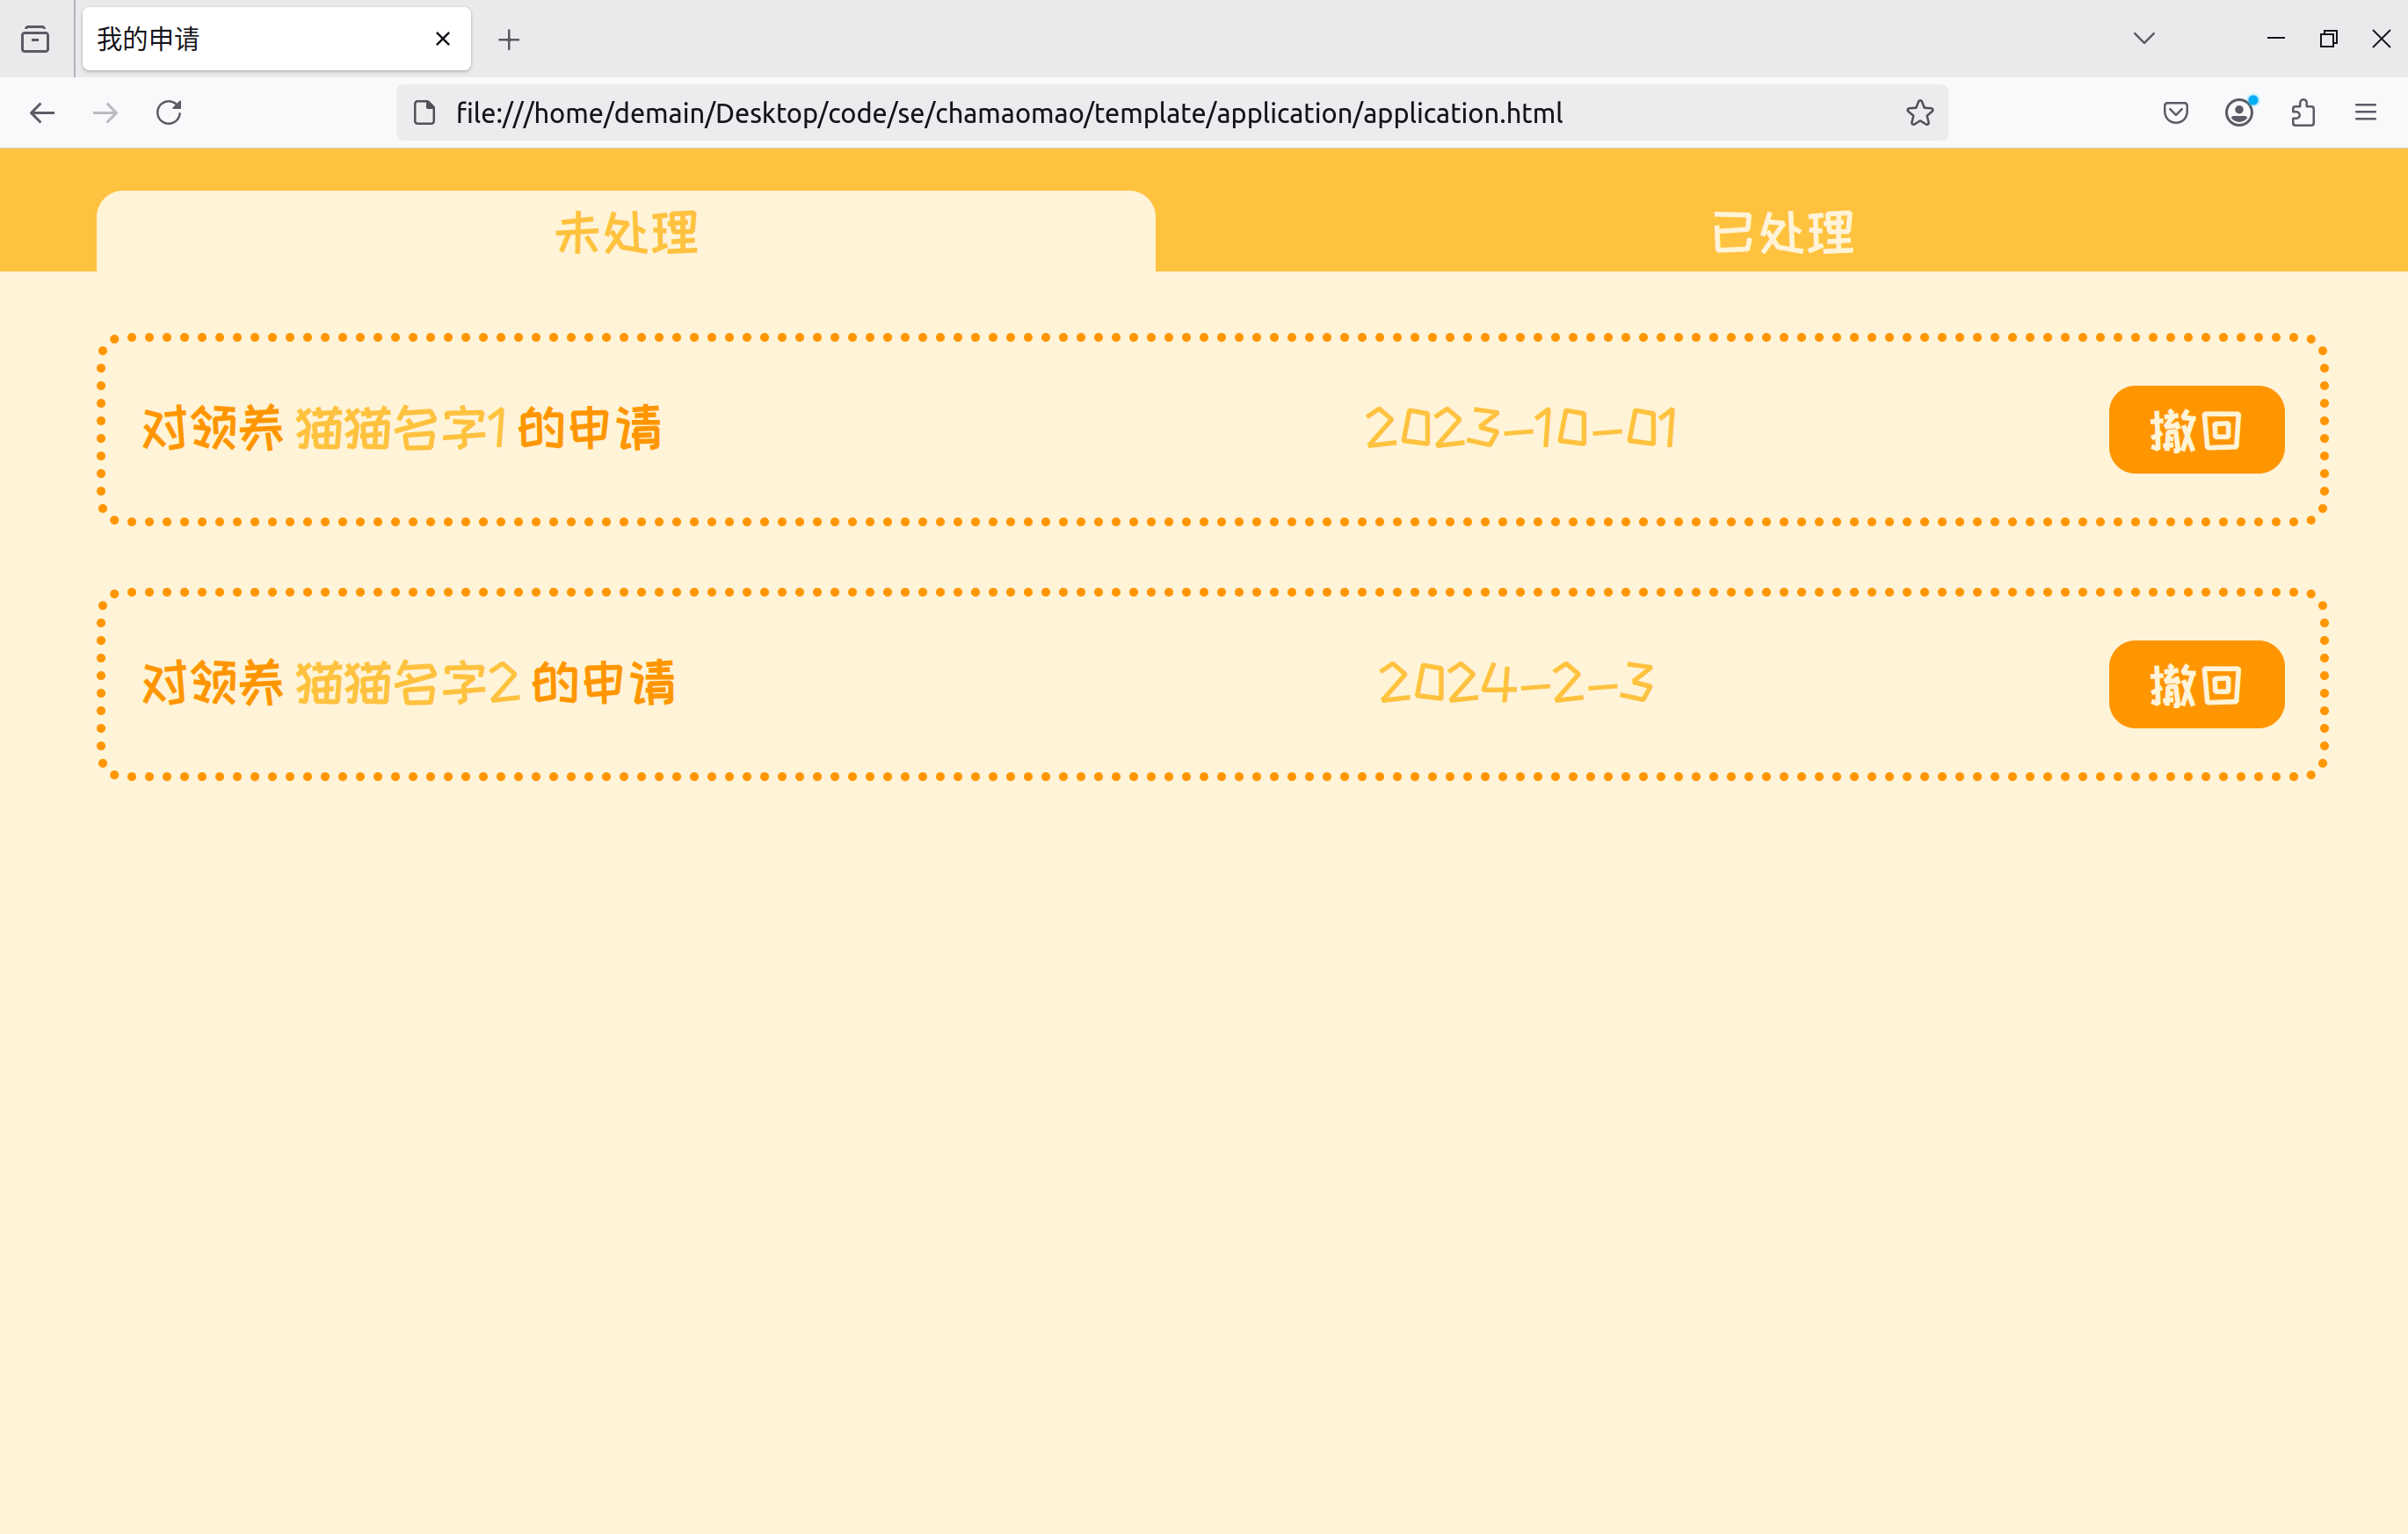
\includegraphics[width=0.9\textwidth]{figures/AdoptionApply1.png}
\end{figure}

\begin{figure}[H]
  \centering
  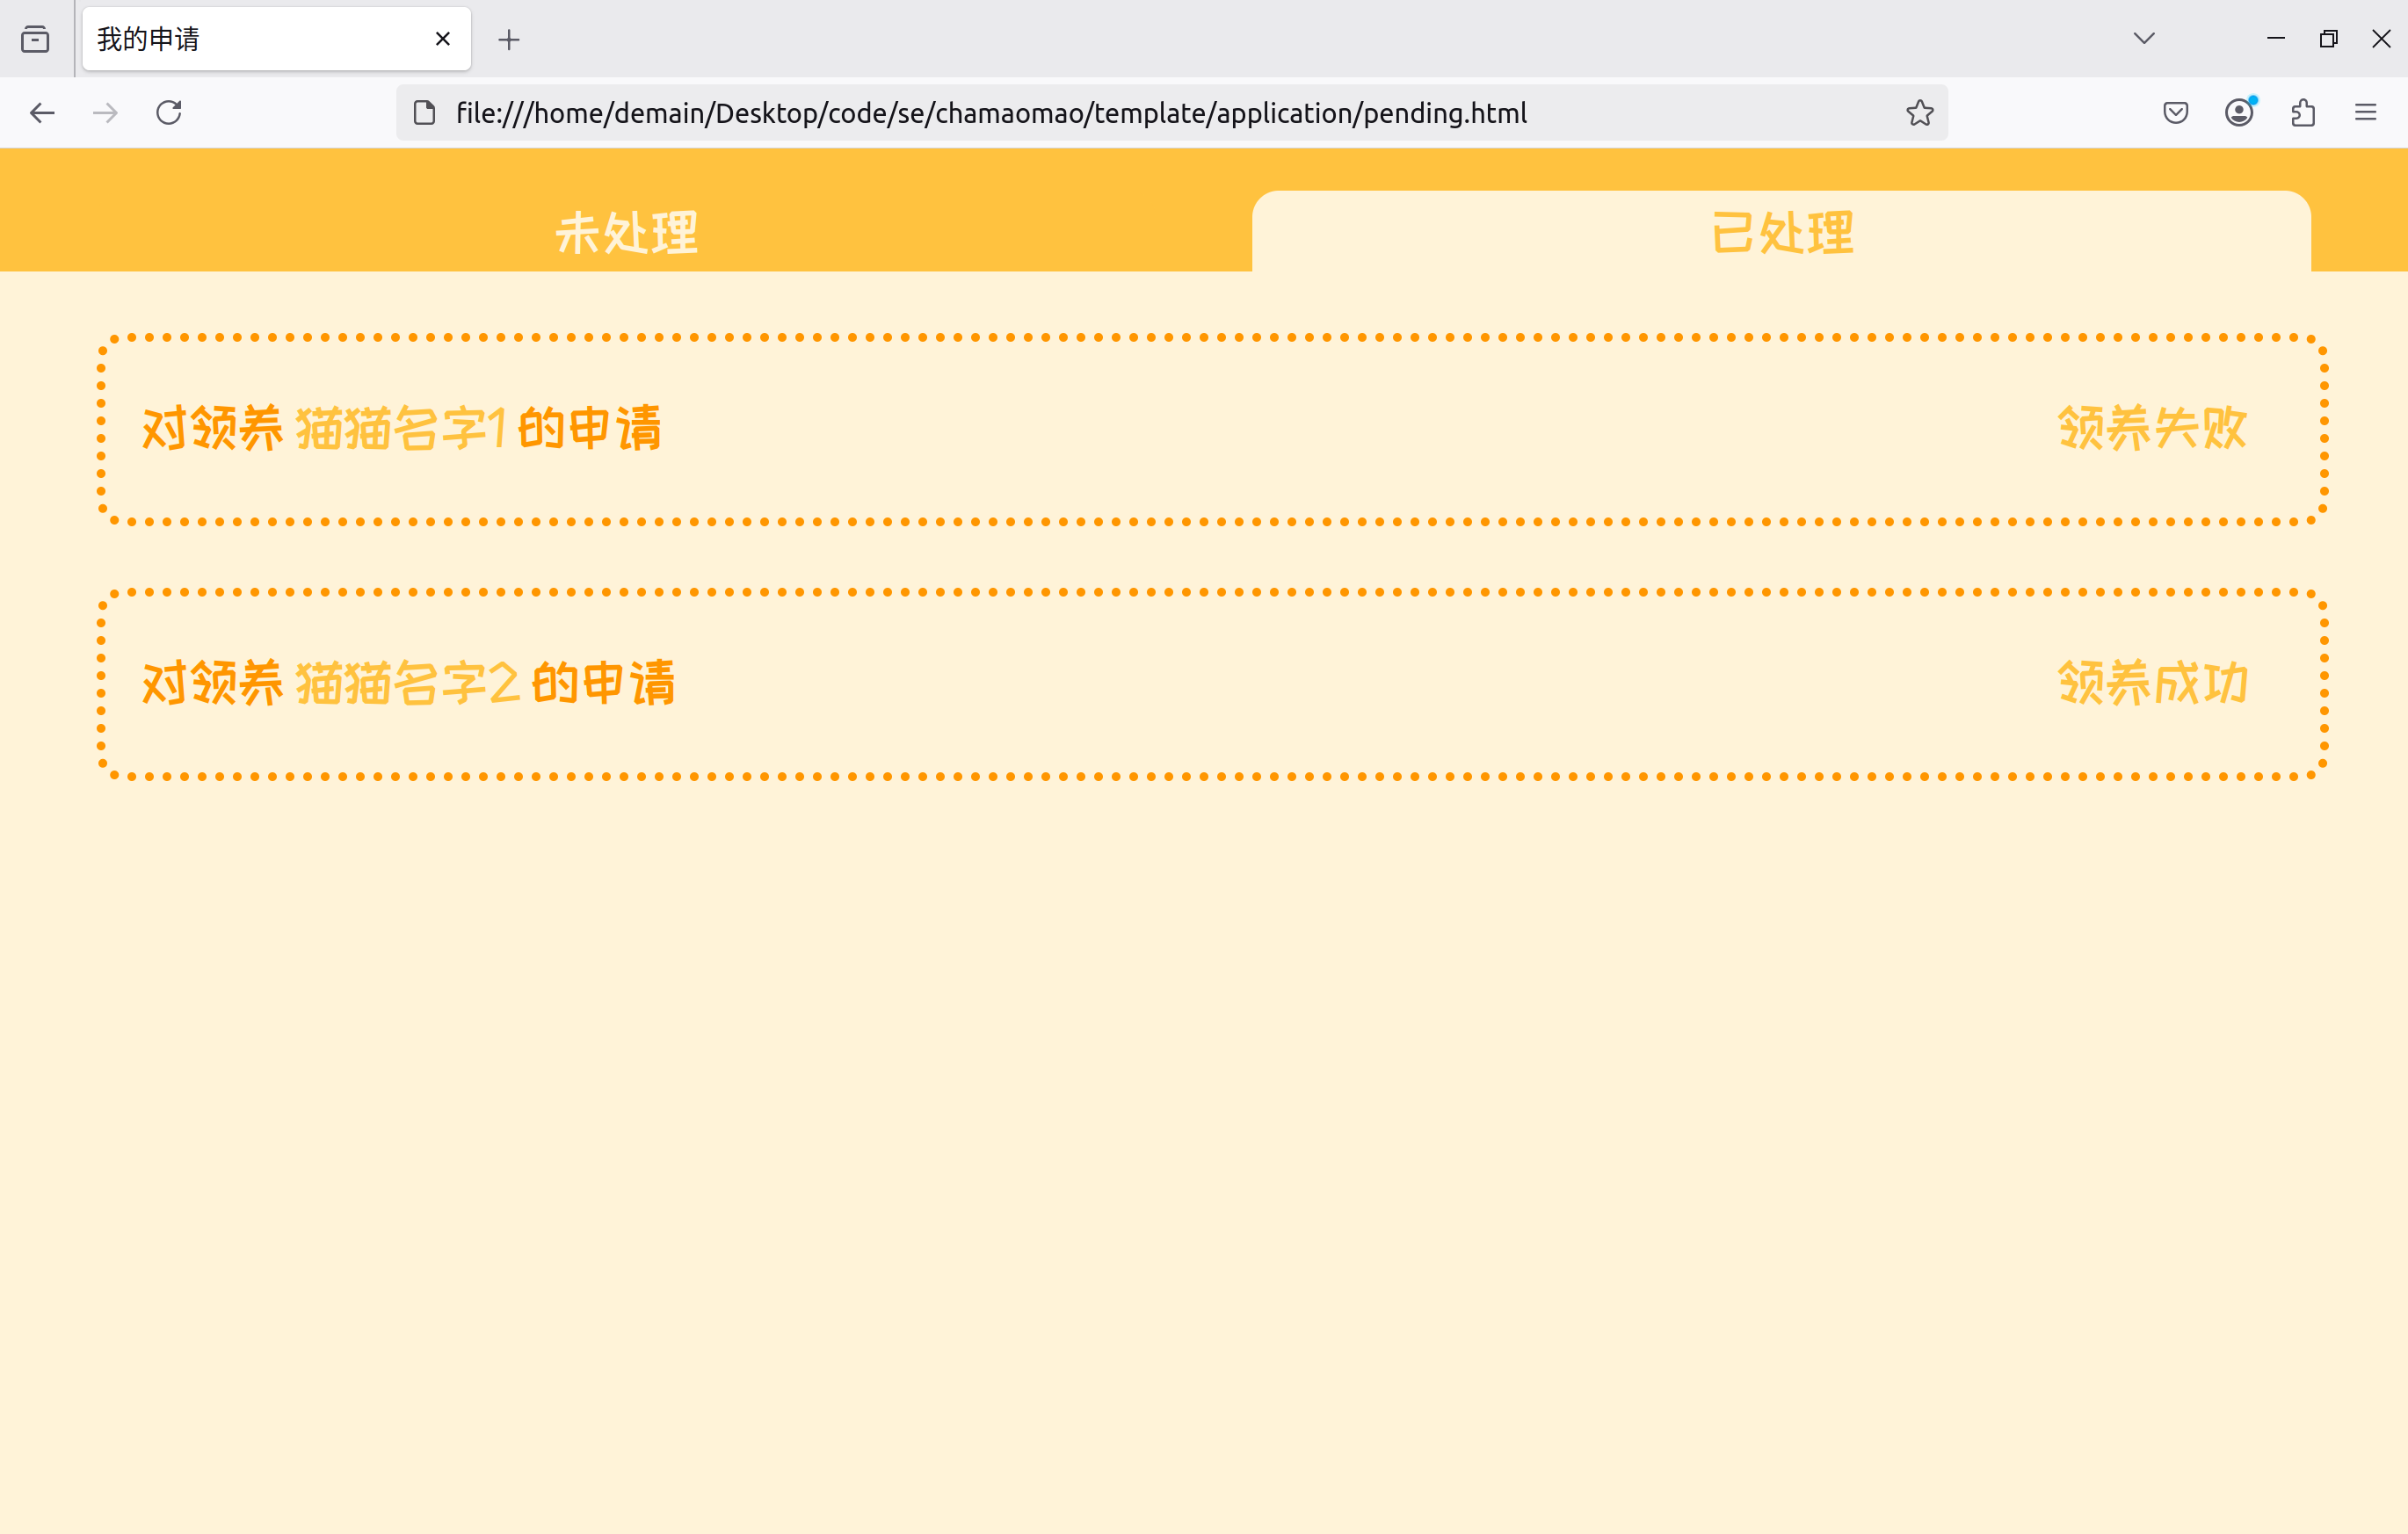
\includegraphics[width=0.9\textwidth]{figures/AdoptionApply2.png}
\end{figure}

\subsubsection{动物地图界面}

\begin{figure}[H]
  \centering
  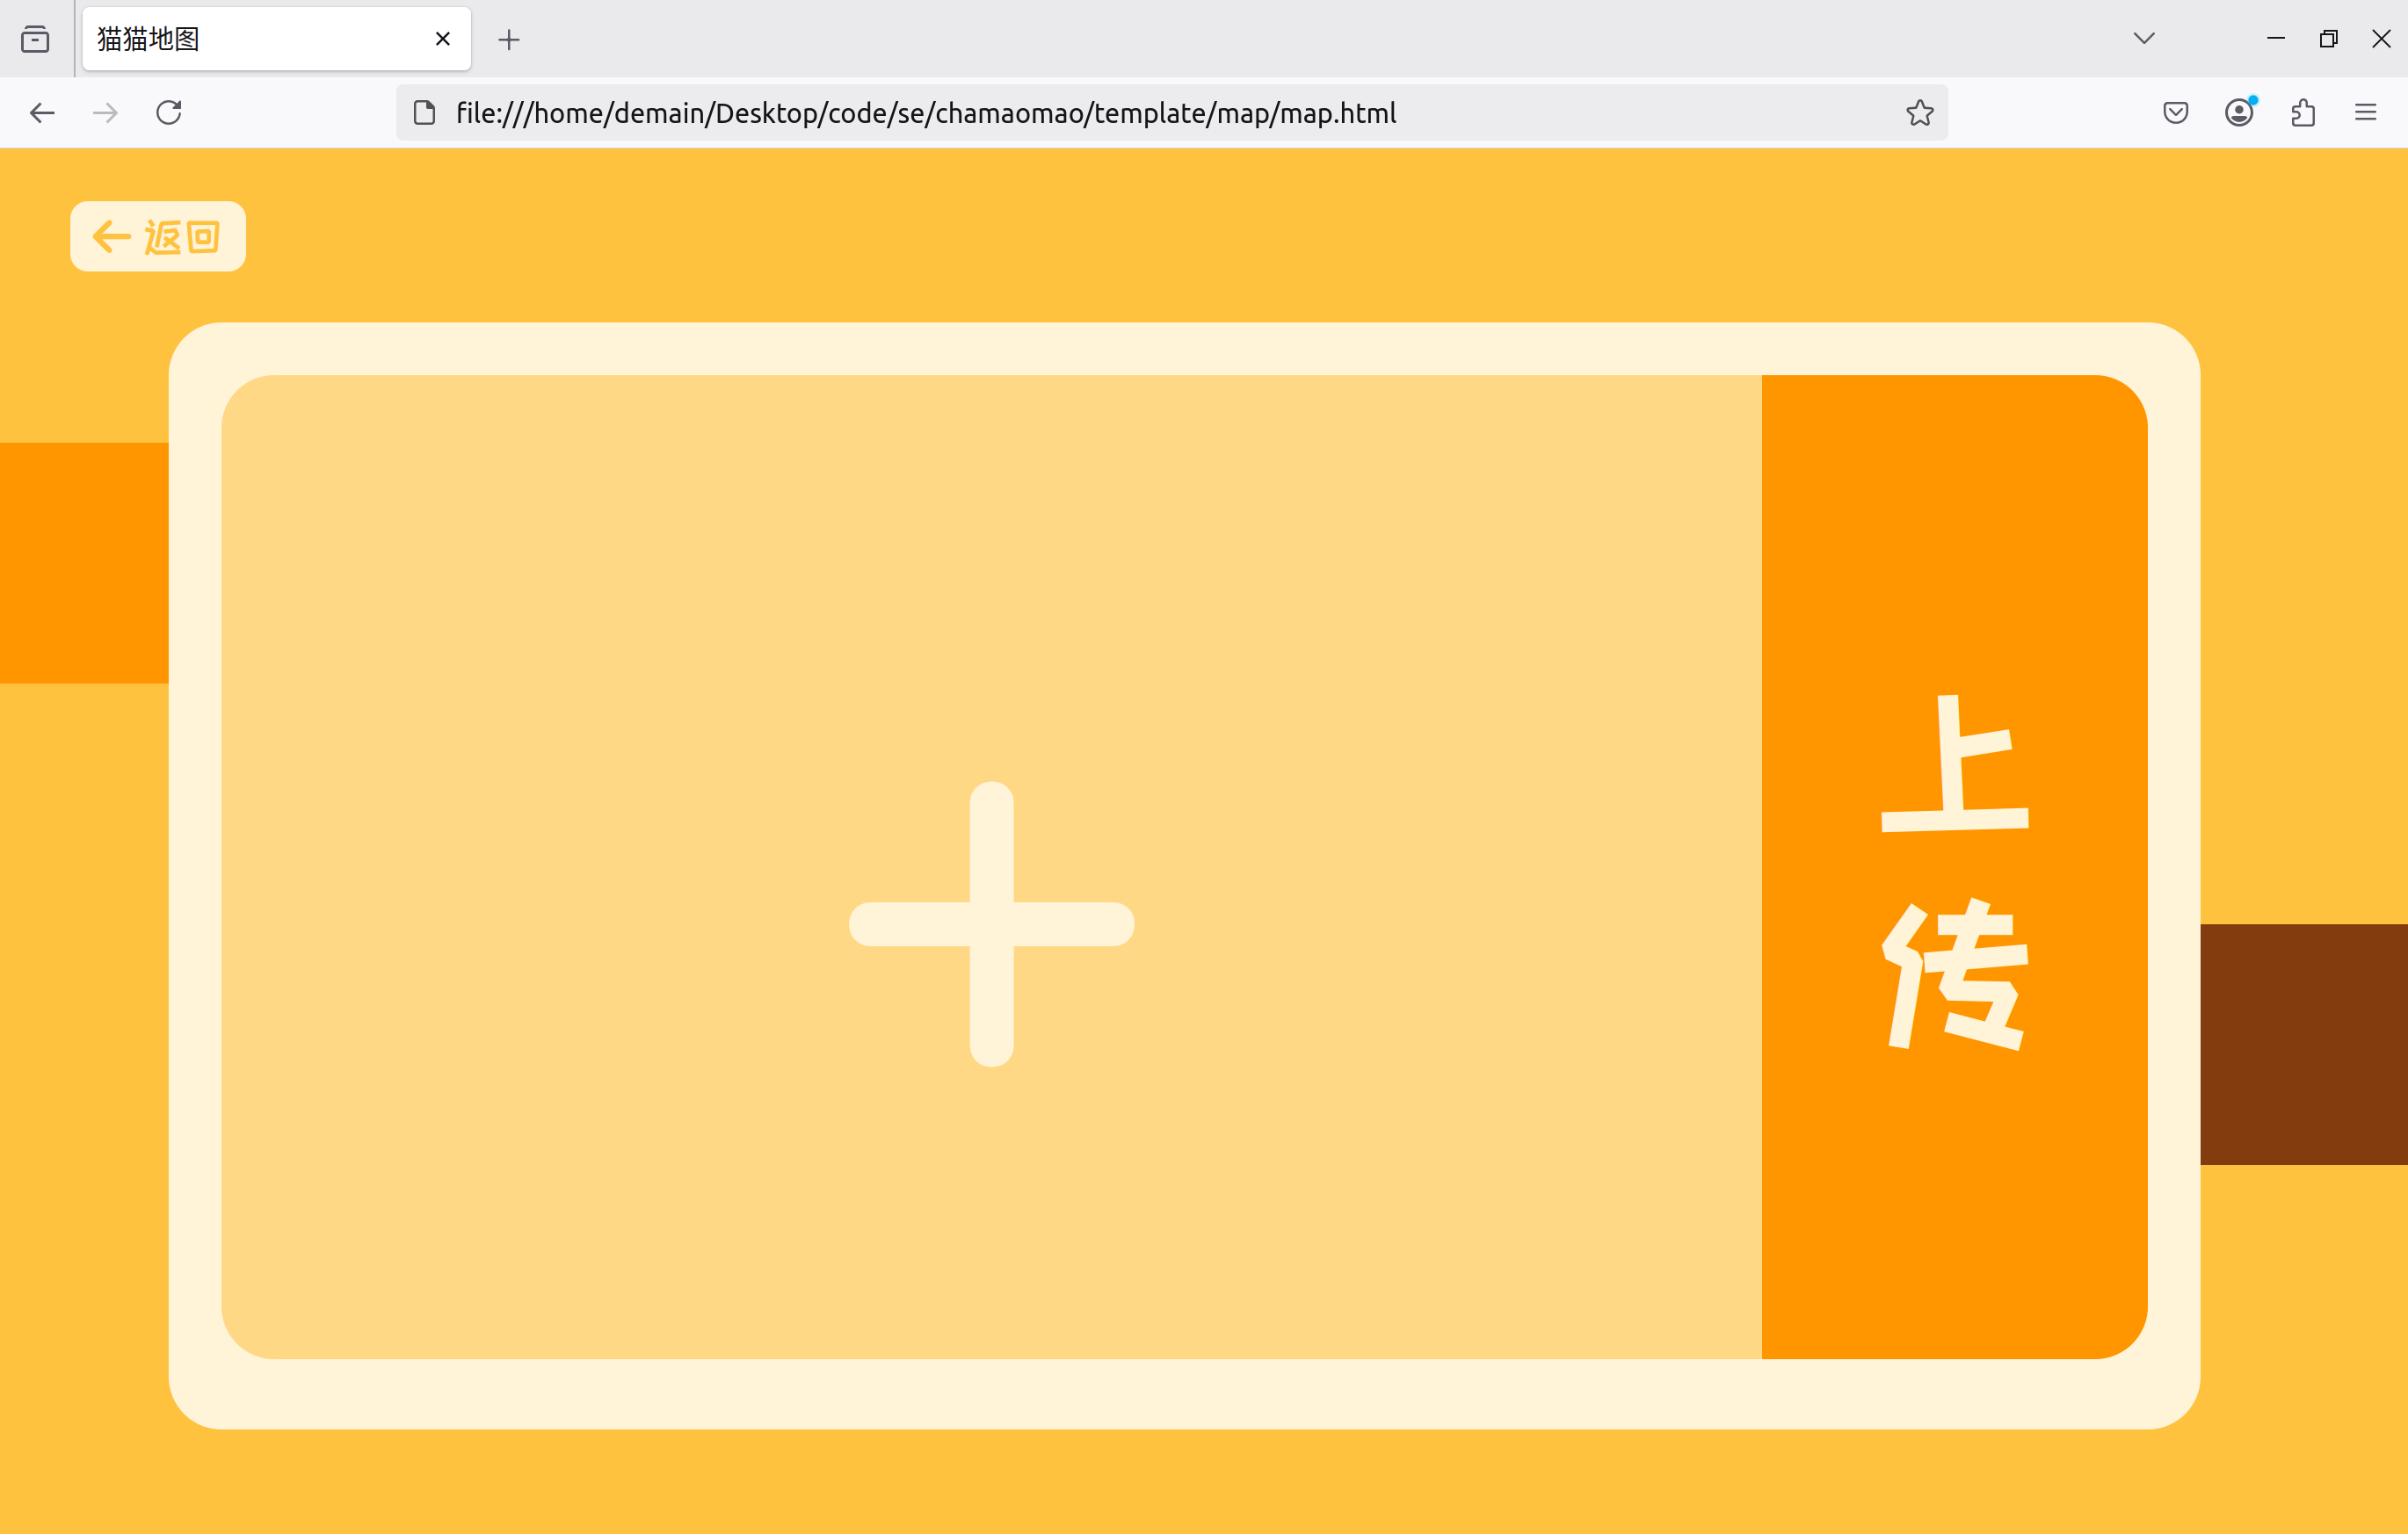
\includegraphics[width=0.9\textwidth]{figures/UserMap.png}
\end{figure}

\subsection{管理员端界面}

\subsubsection{登录界面}

\begin{figure}[H]
  \centering
  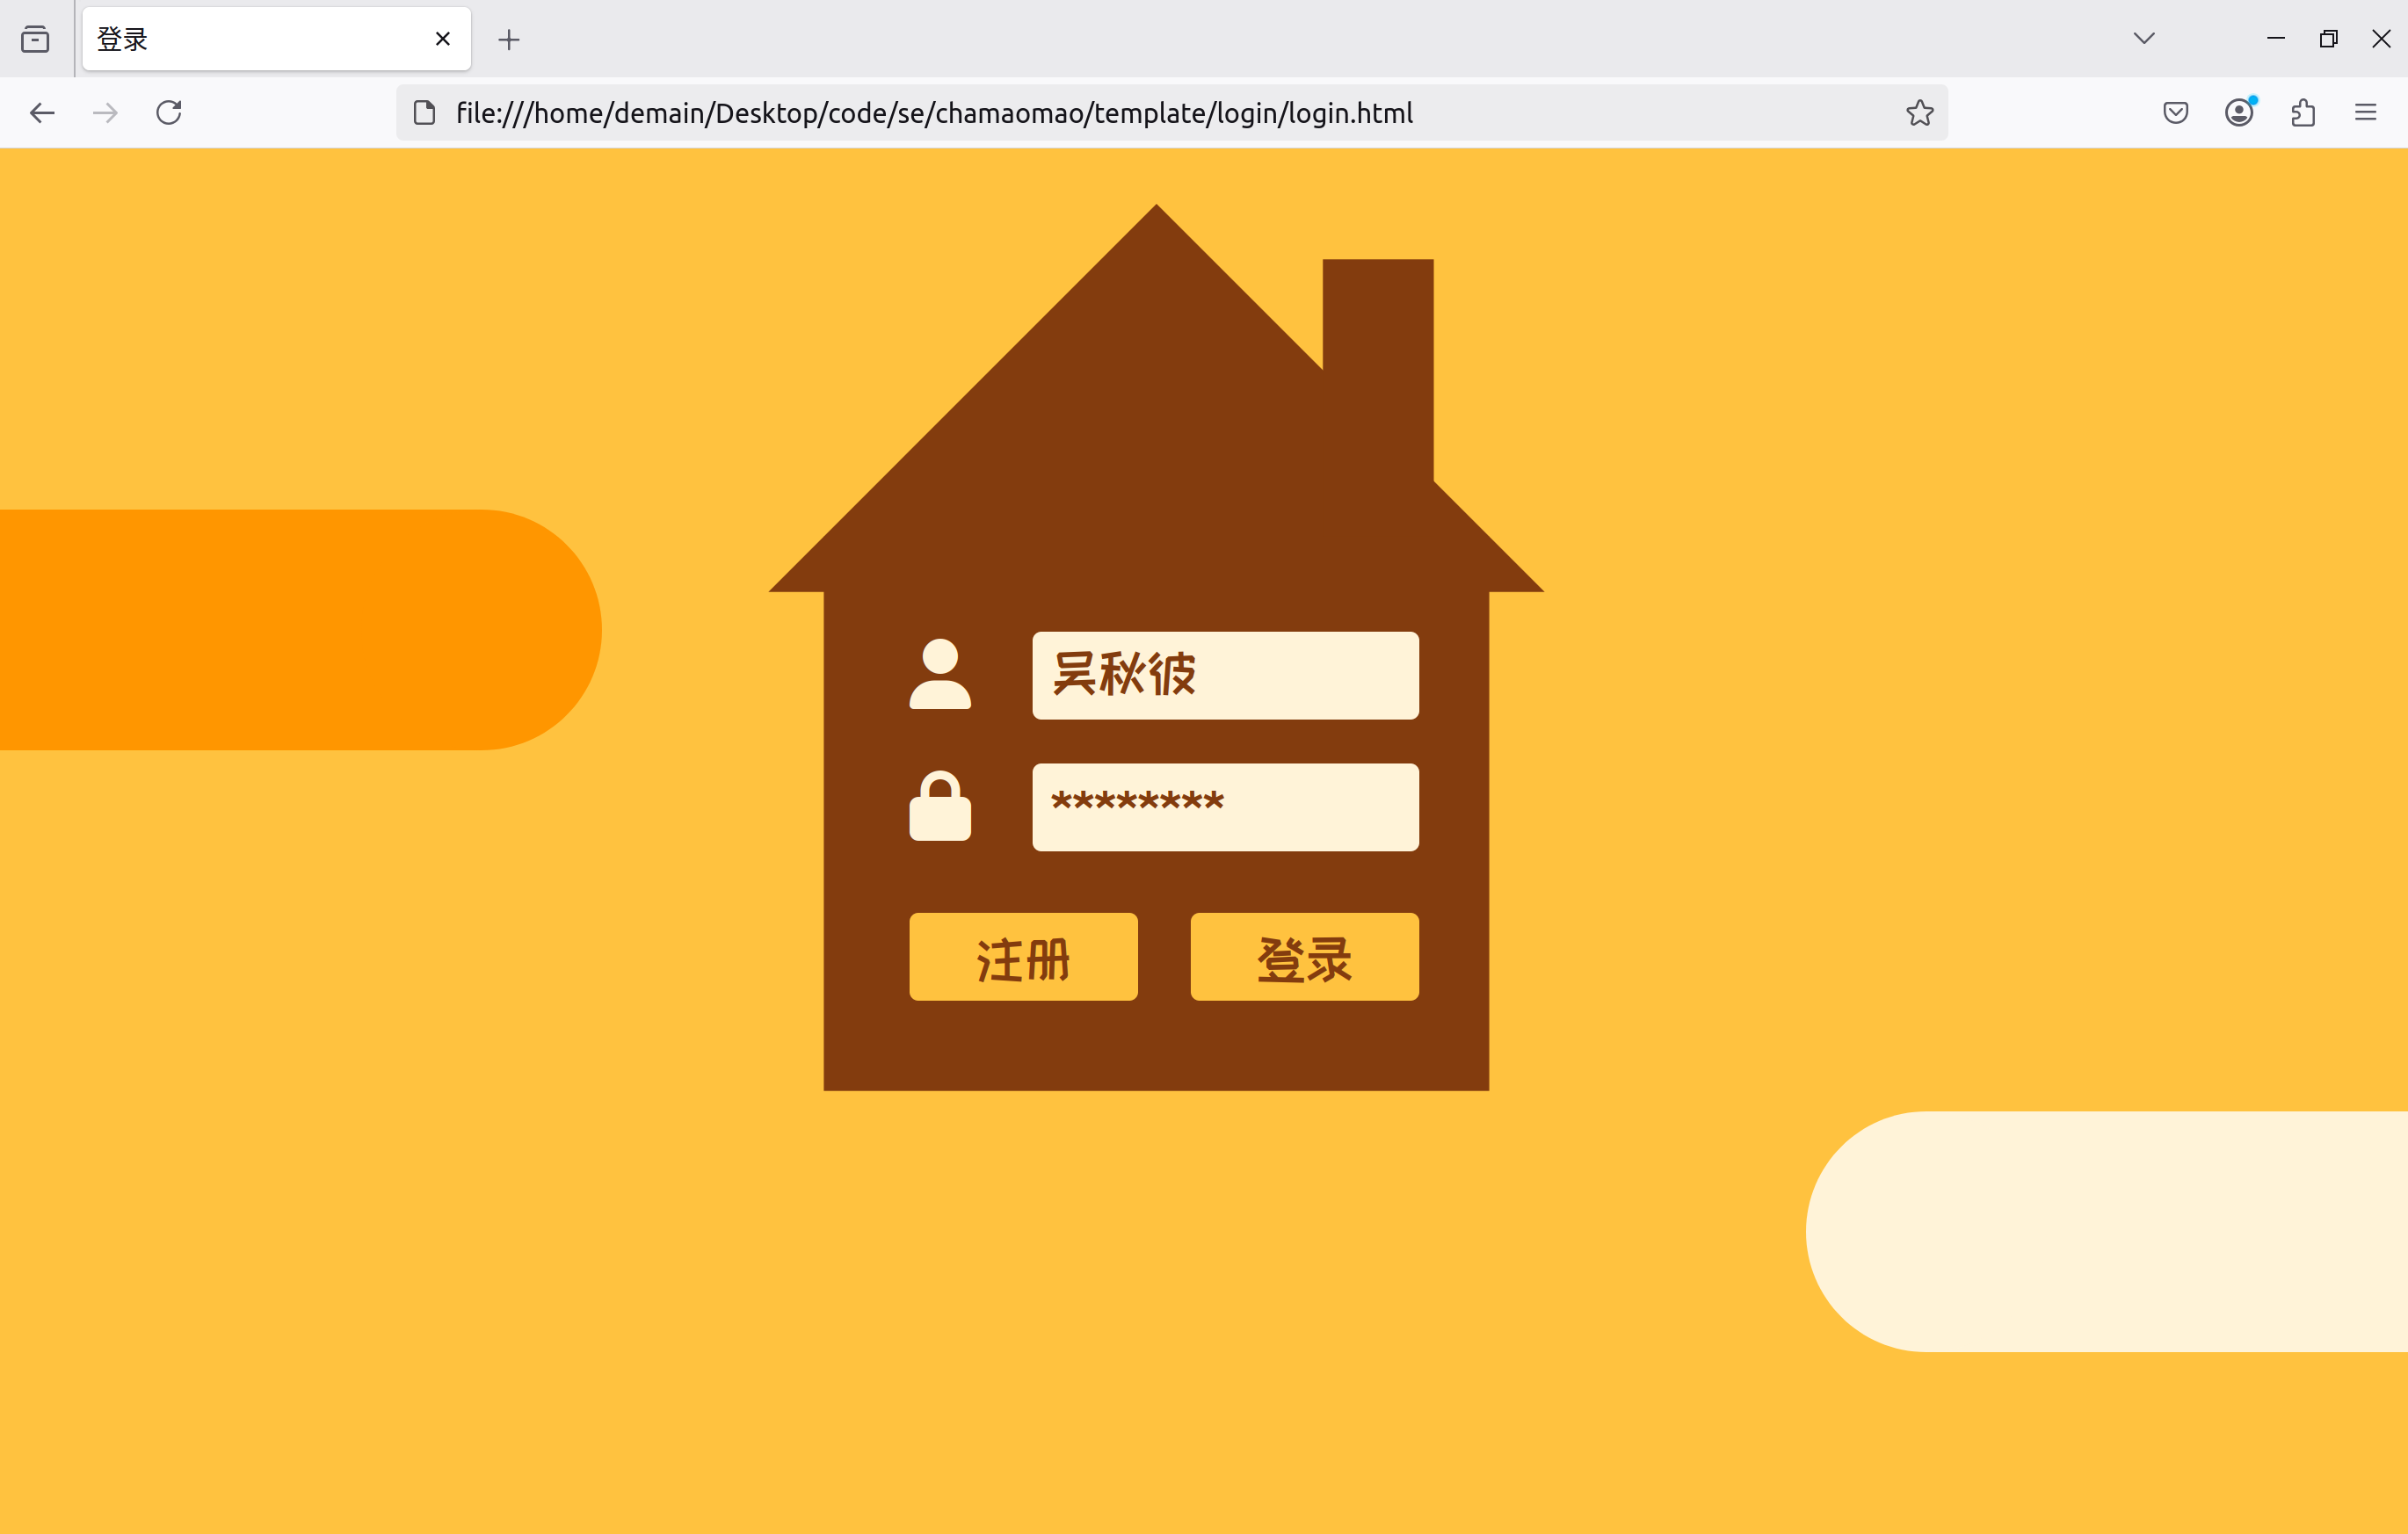
\includegraphics[width=0.9\textwidth]{figures/UserLogin.png}
\end{figure}

\subsubsection{动物信息管理界面}

\begin{figure}[H]
  \centering
  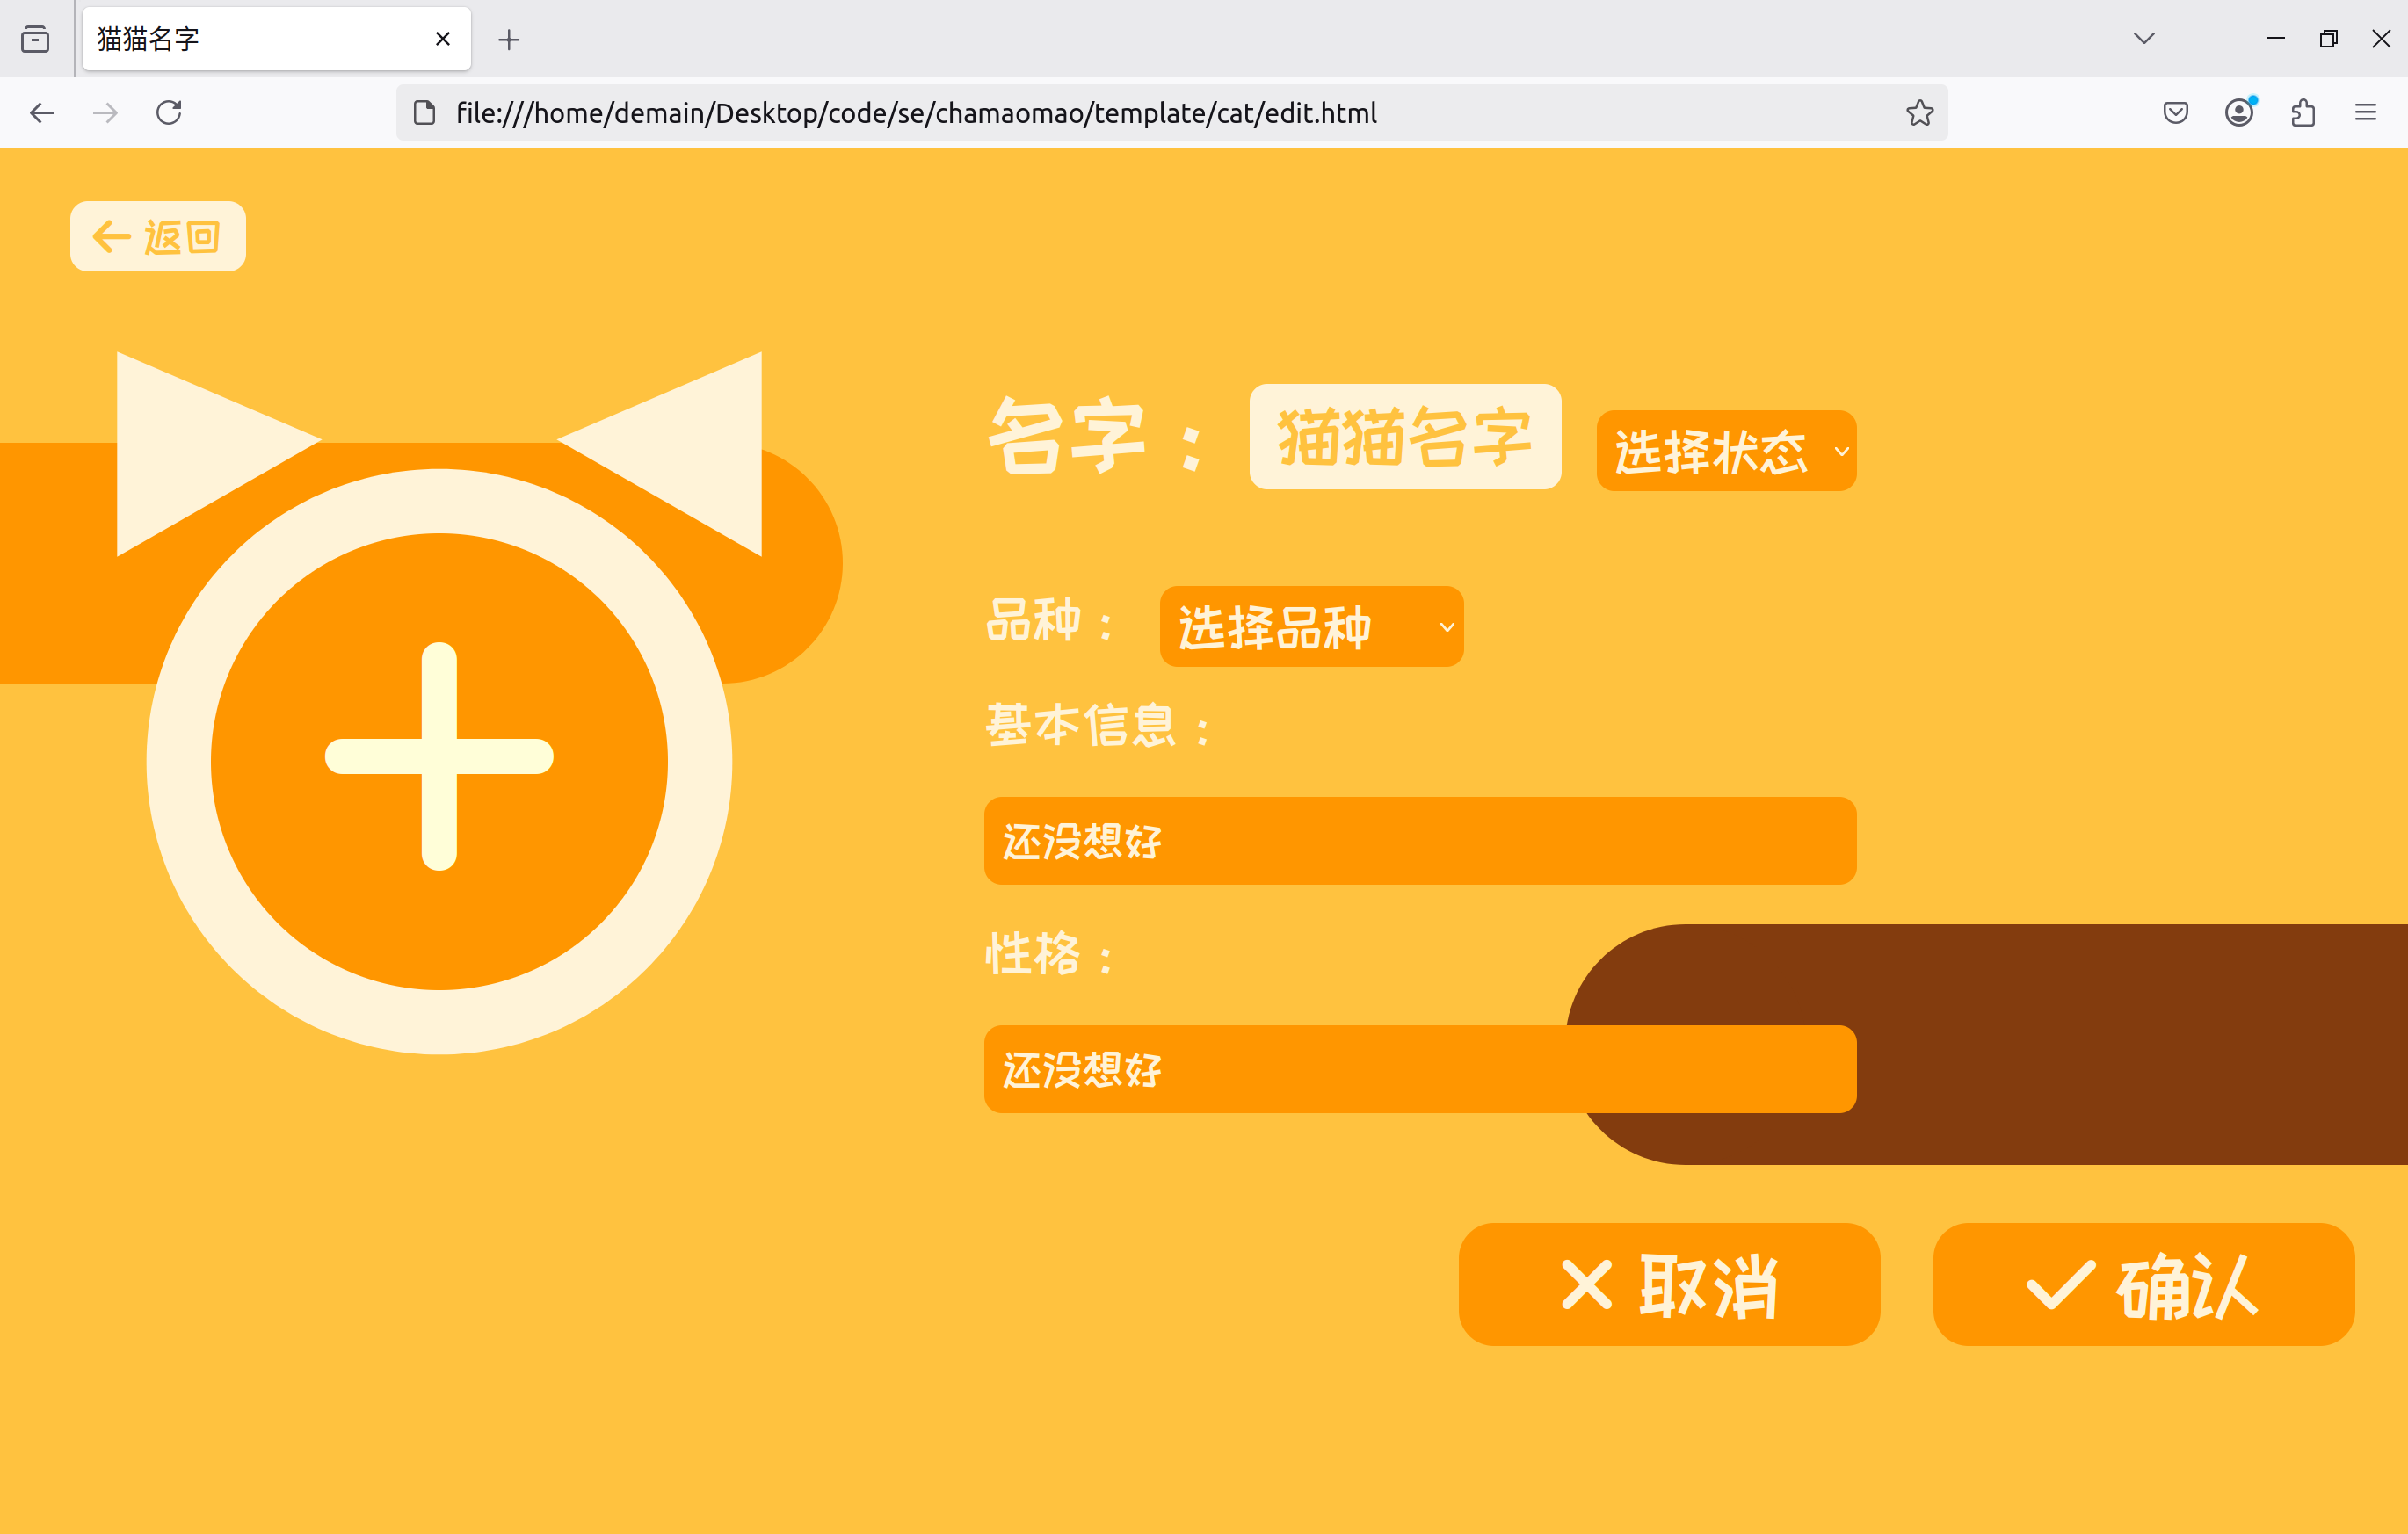
\includegraphics[width=0.9\textwidth]{figures/AnimalInfo4.png}
\end{figure}

\subsubsection{动物信息浏览界面}

\begin{figure}[H]
  \centering
  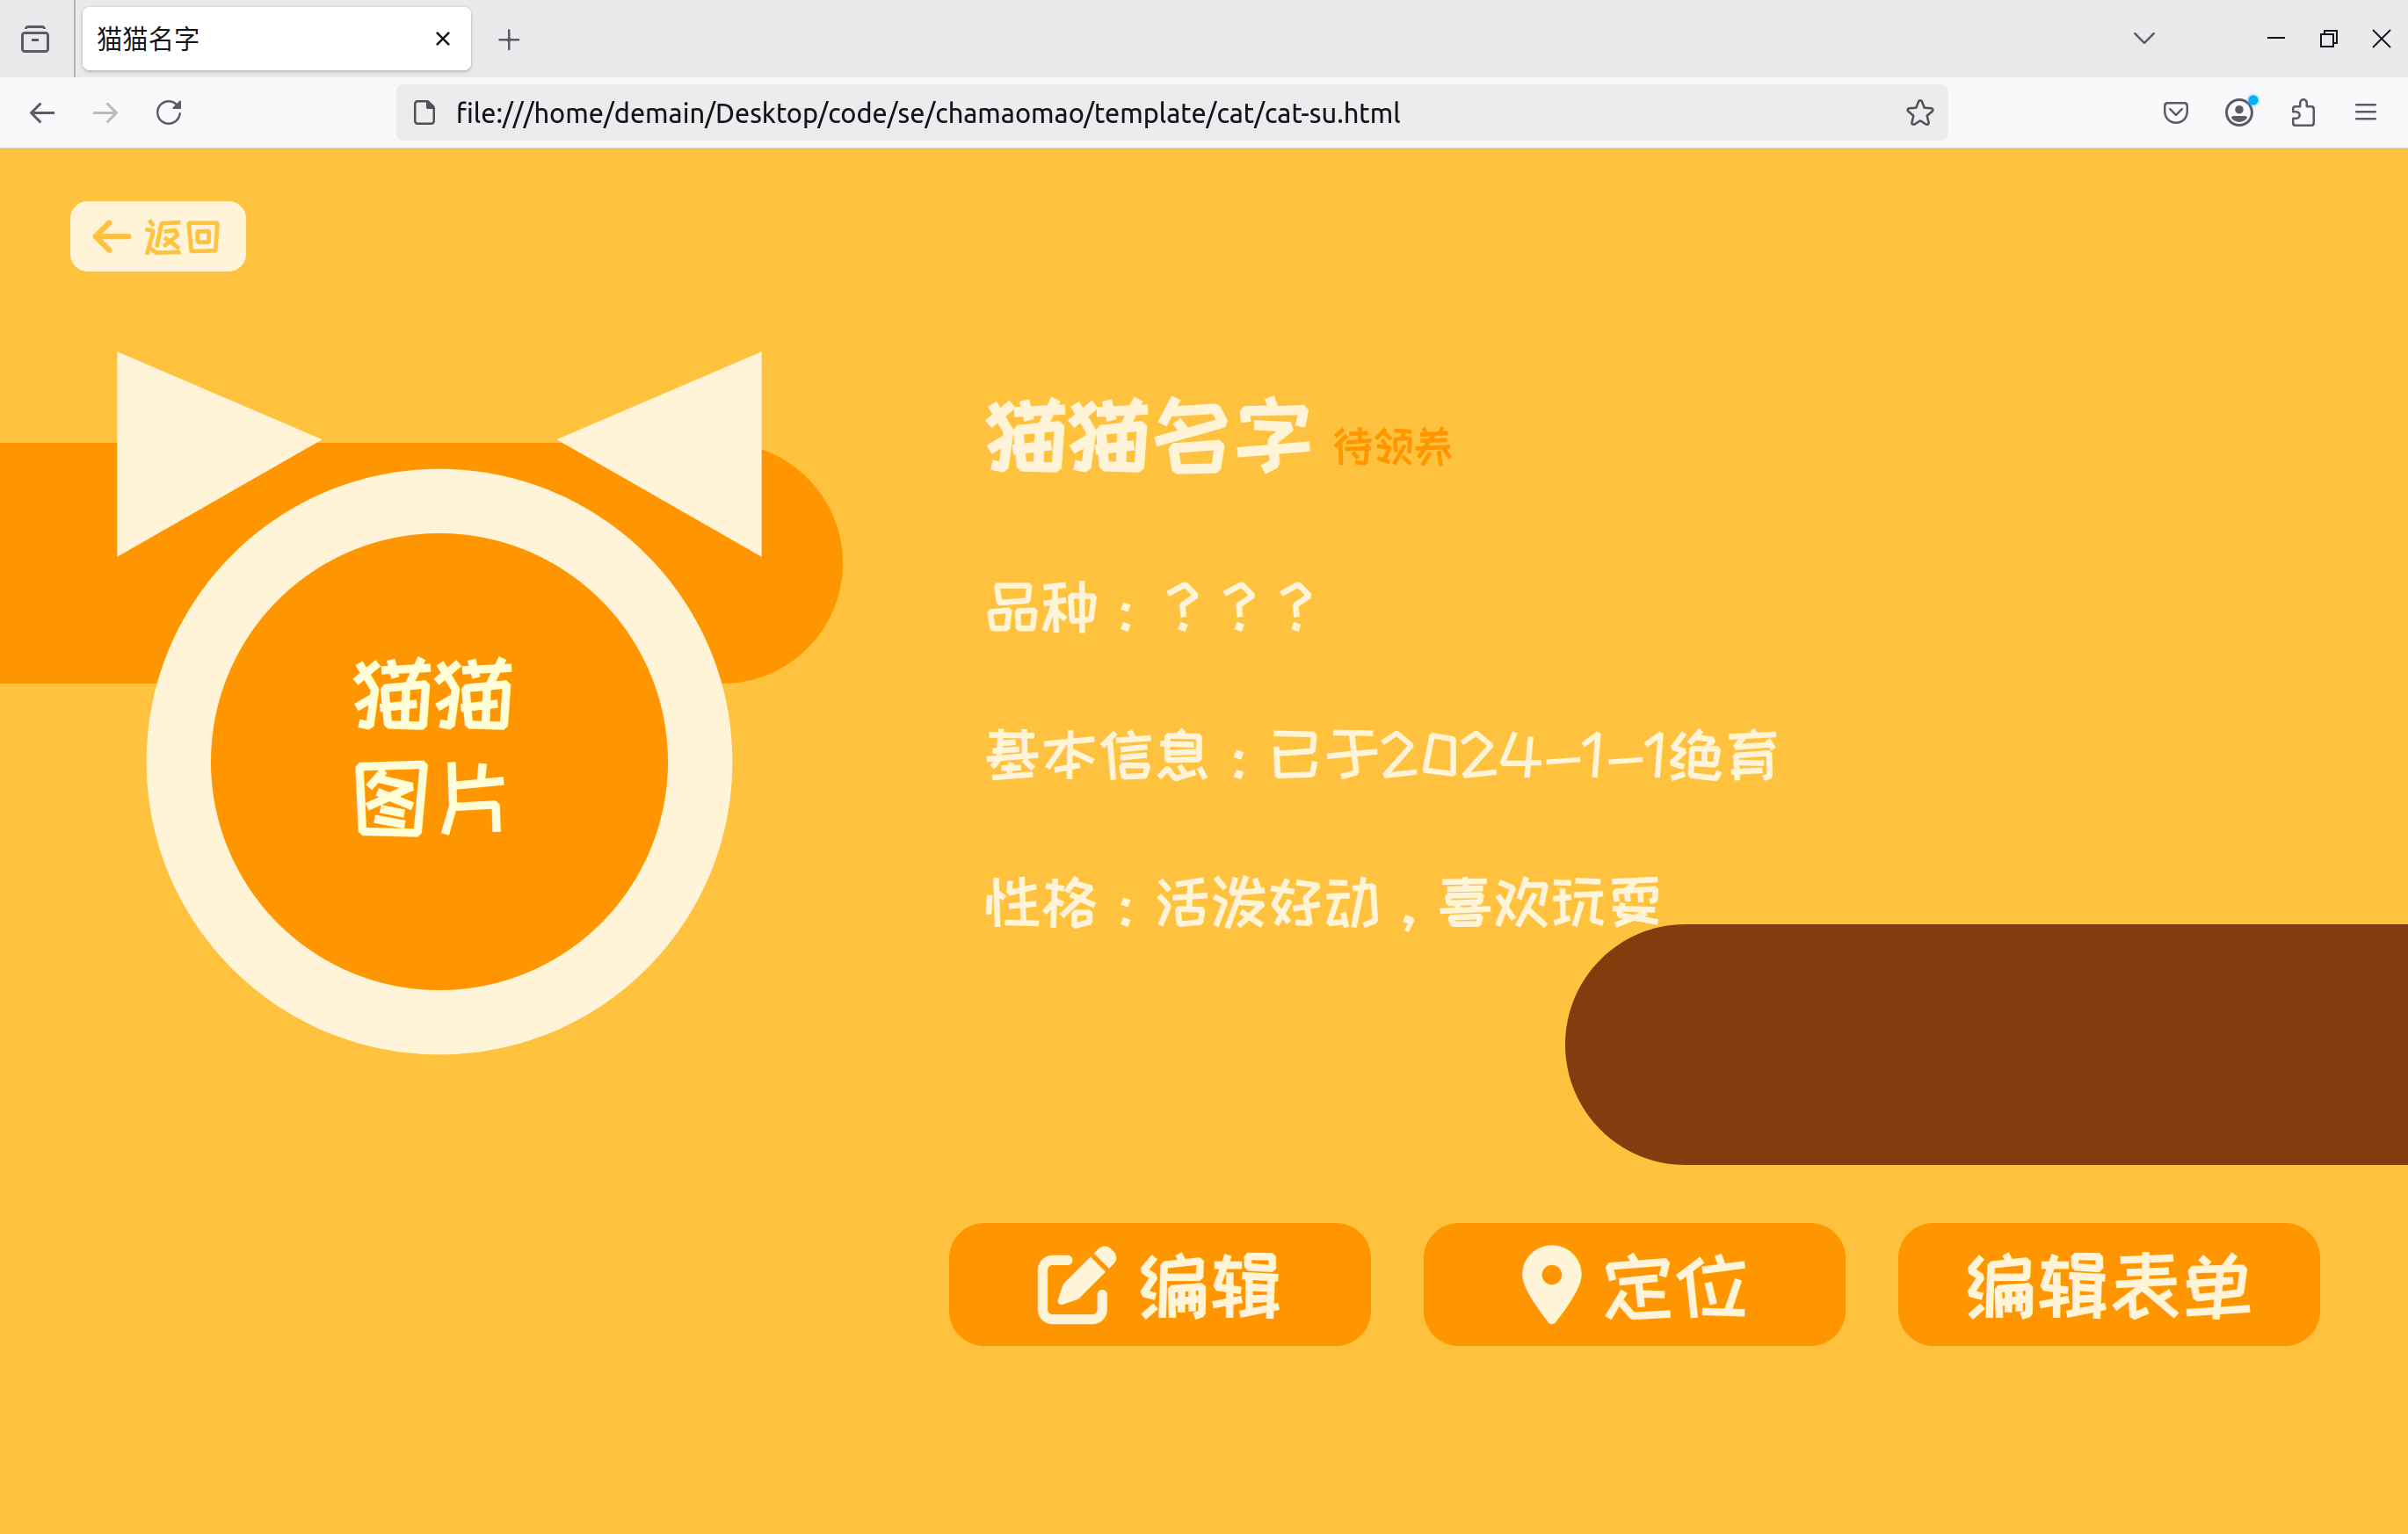
\includegraphics[width=0.9\textwidth]{figures/AnimalInfo3.png}
\end{figure}

\subsubsection{领养申请审批界面}

\begin{figure}[H]
  \centering
  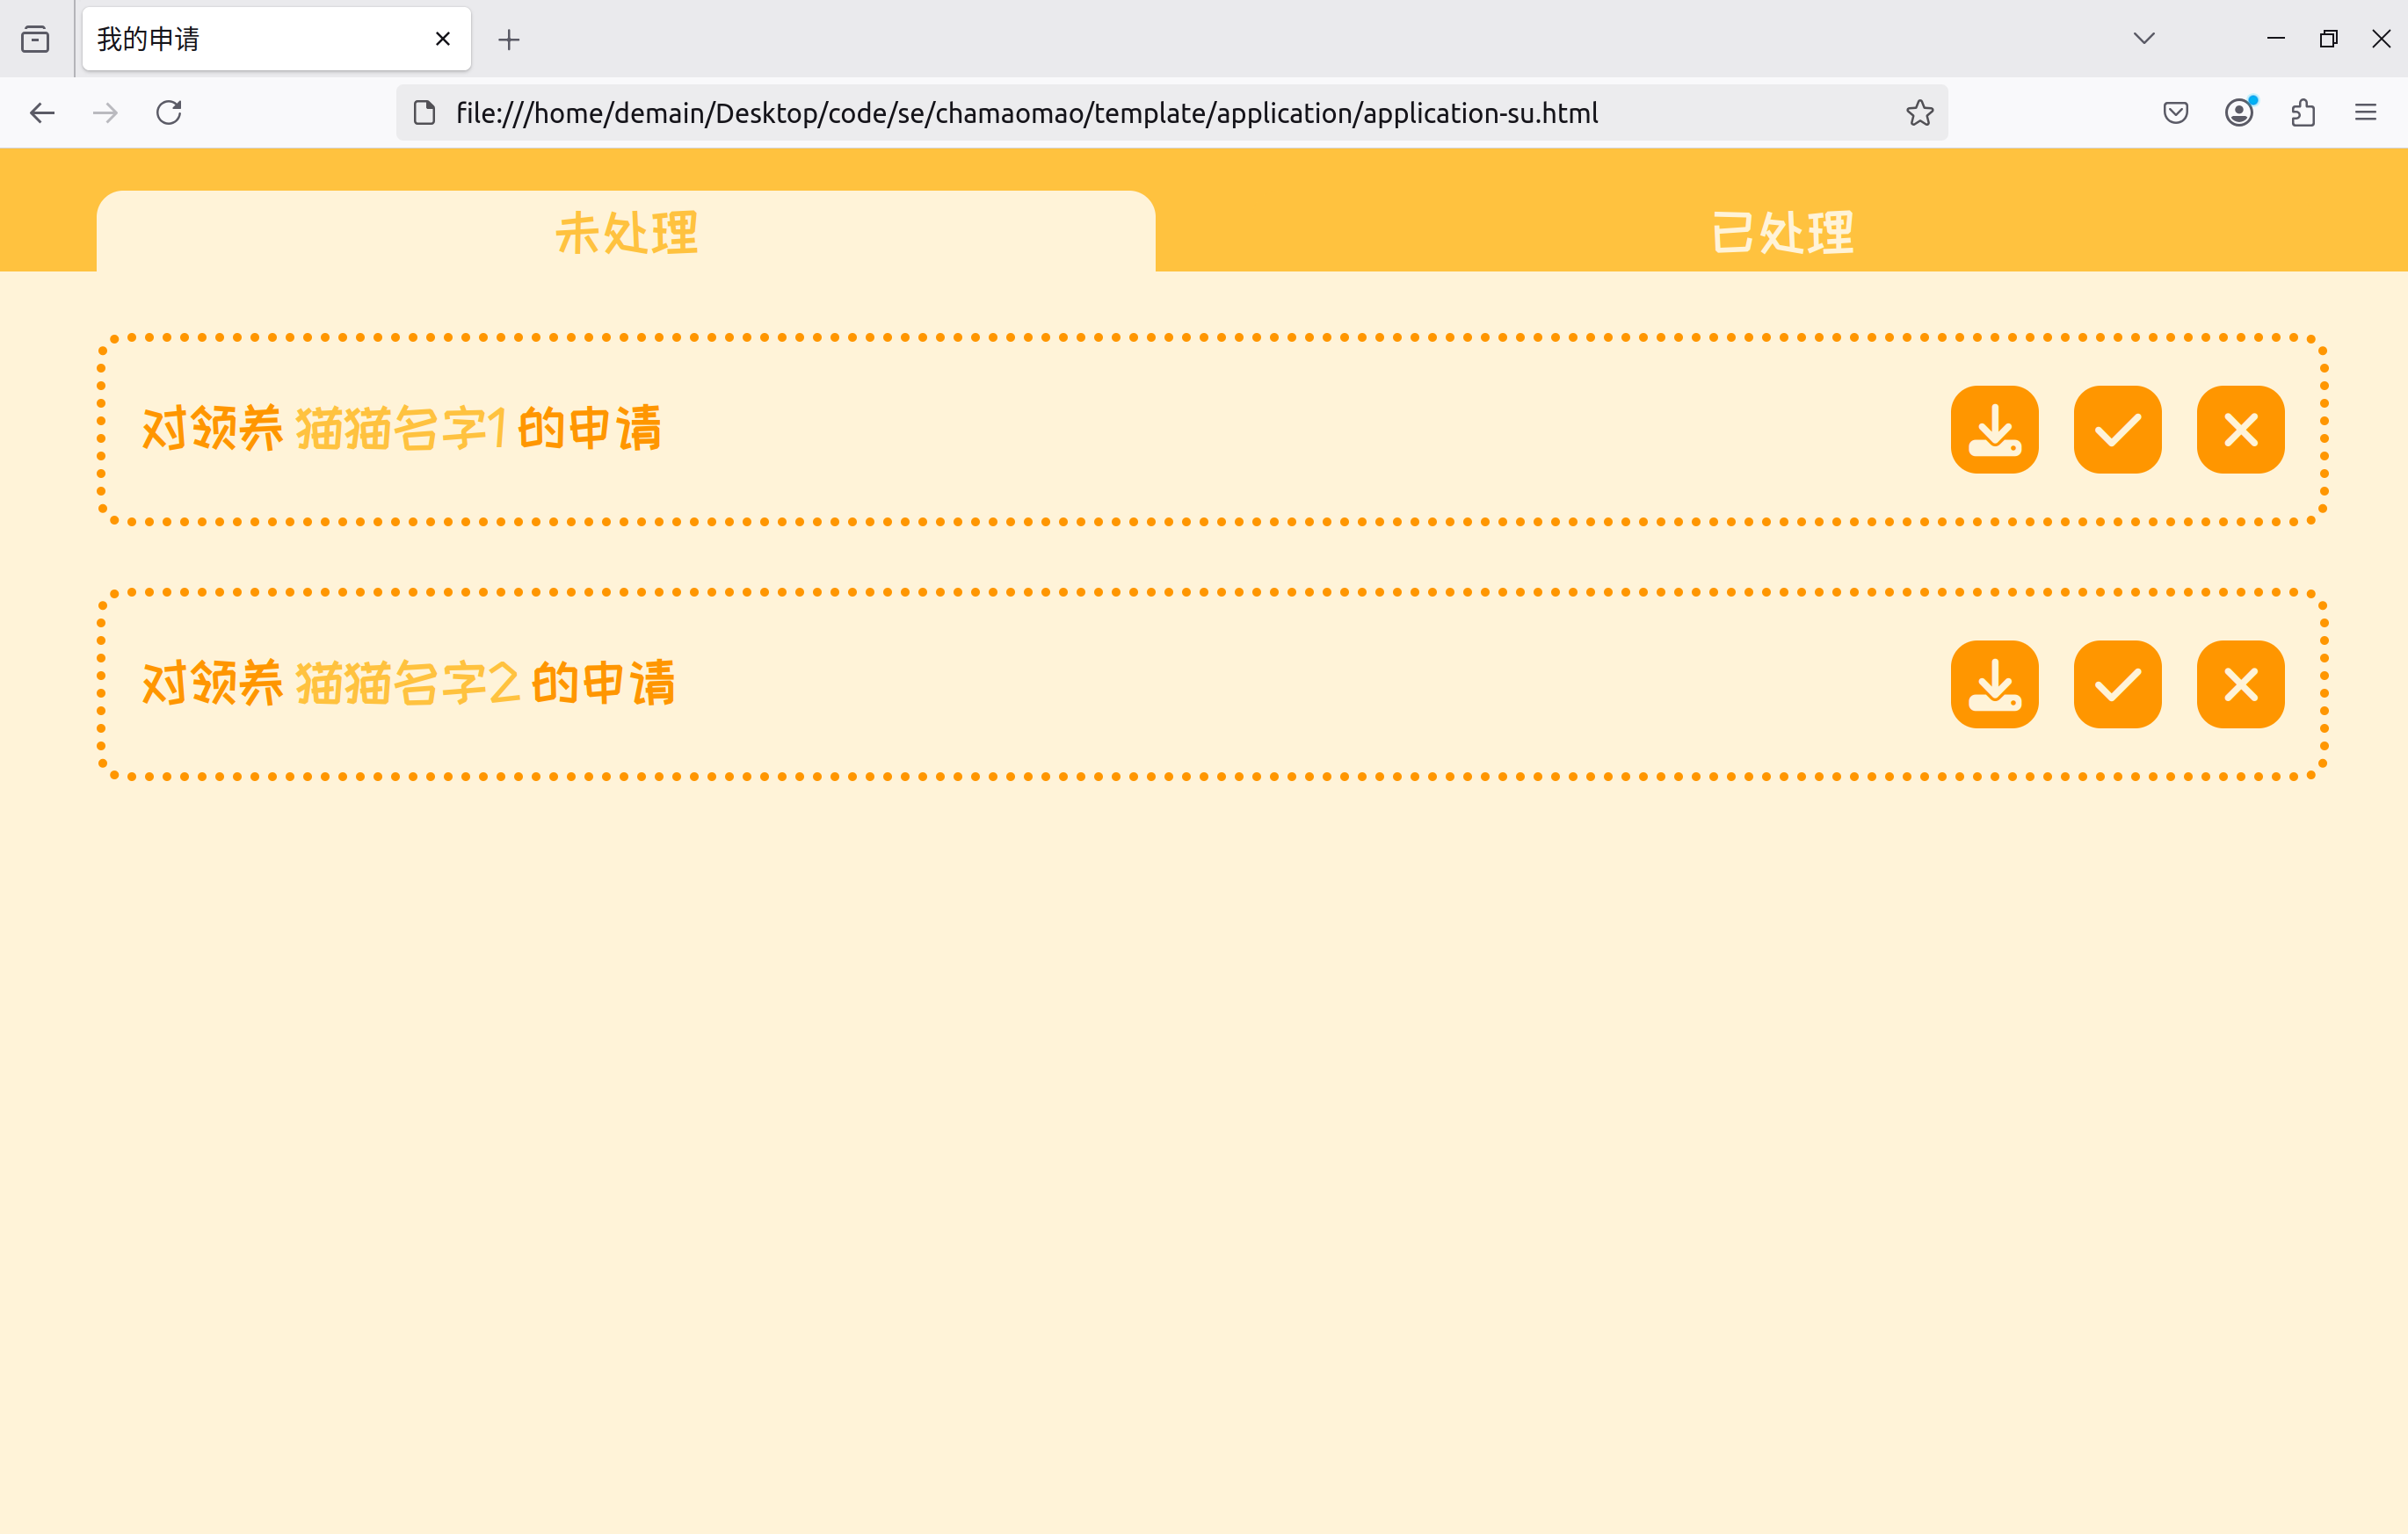
\includegraphics[width=0.9\textwidth]{figures/AdoptionApply3.png}
\end{figure}

\begin{figure}[H]
  \centering
  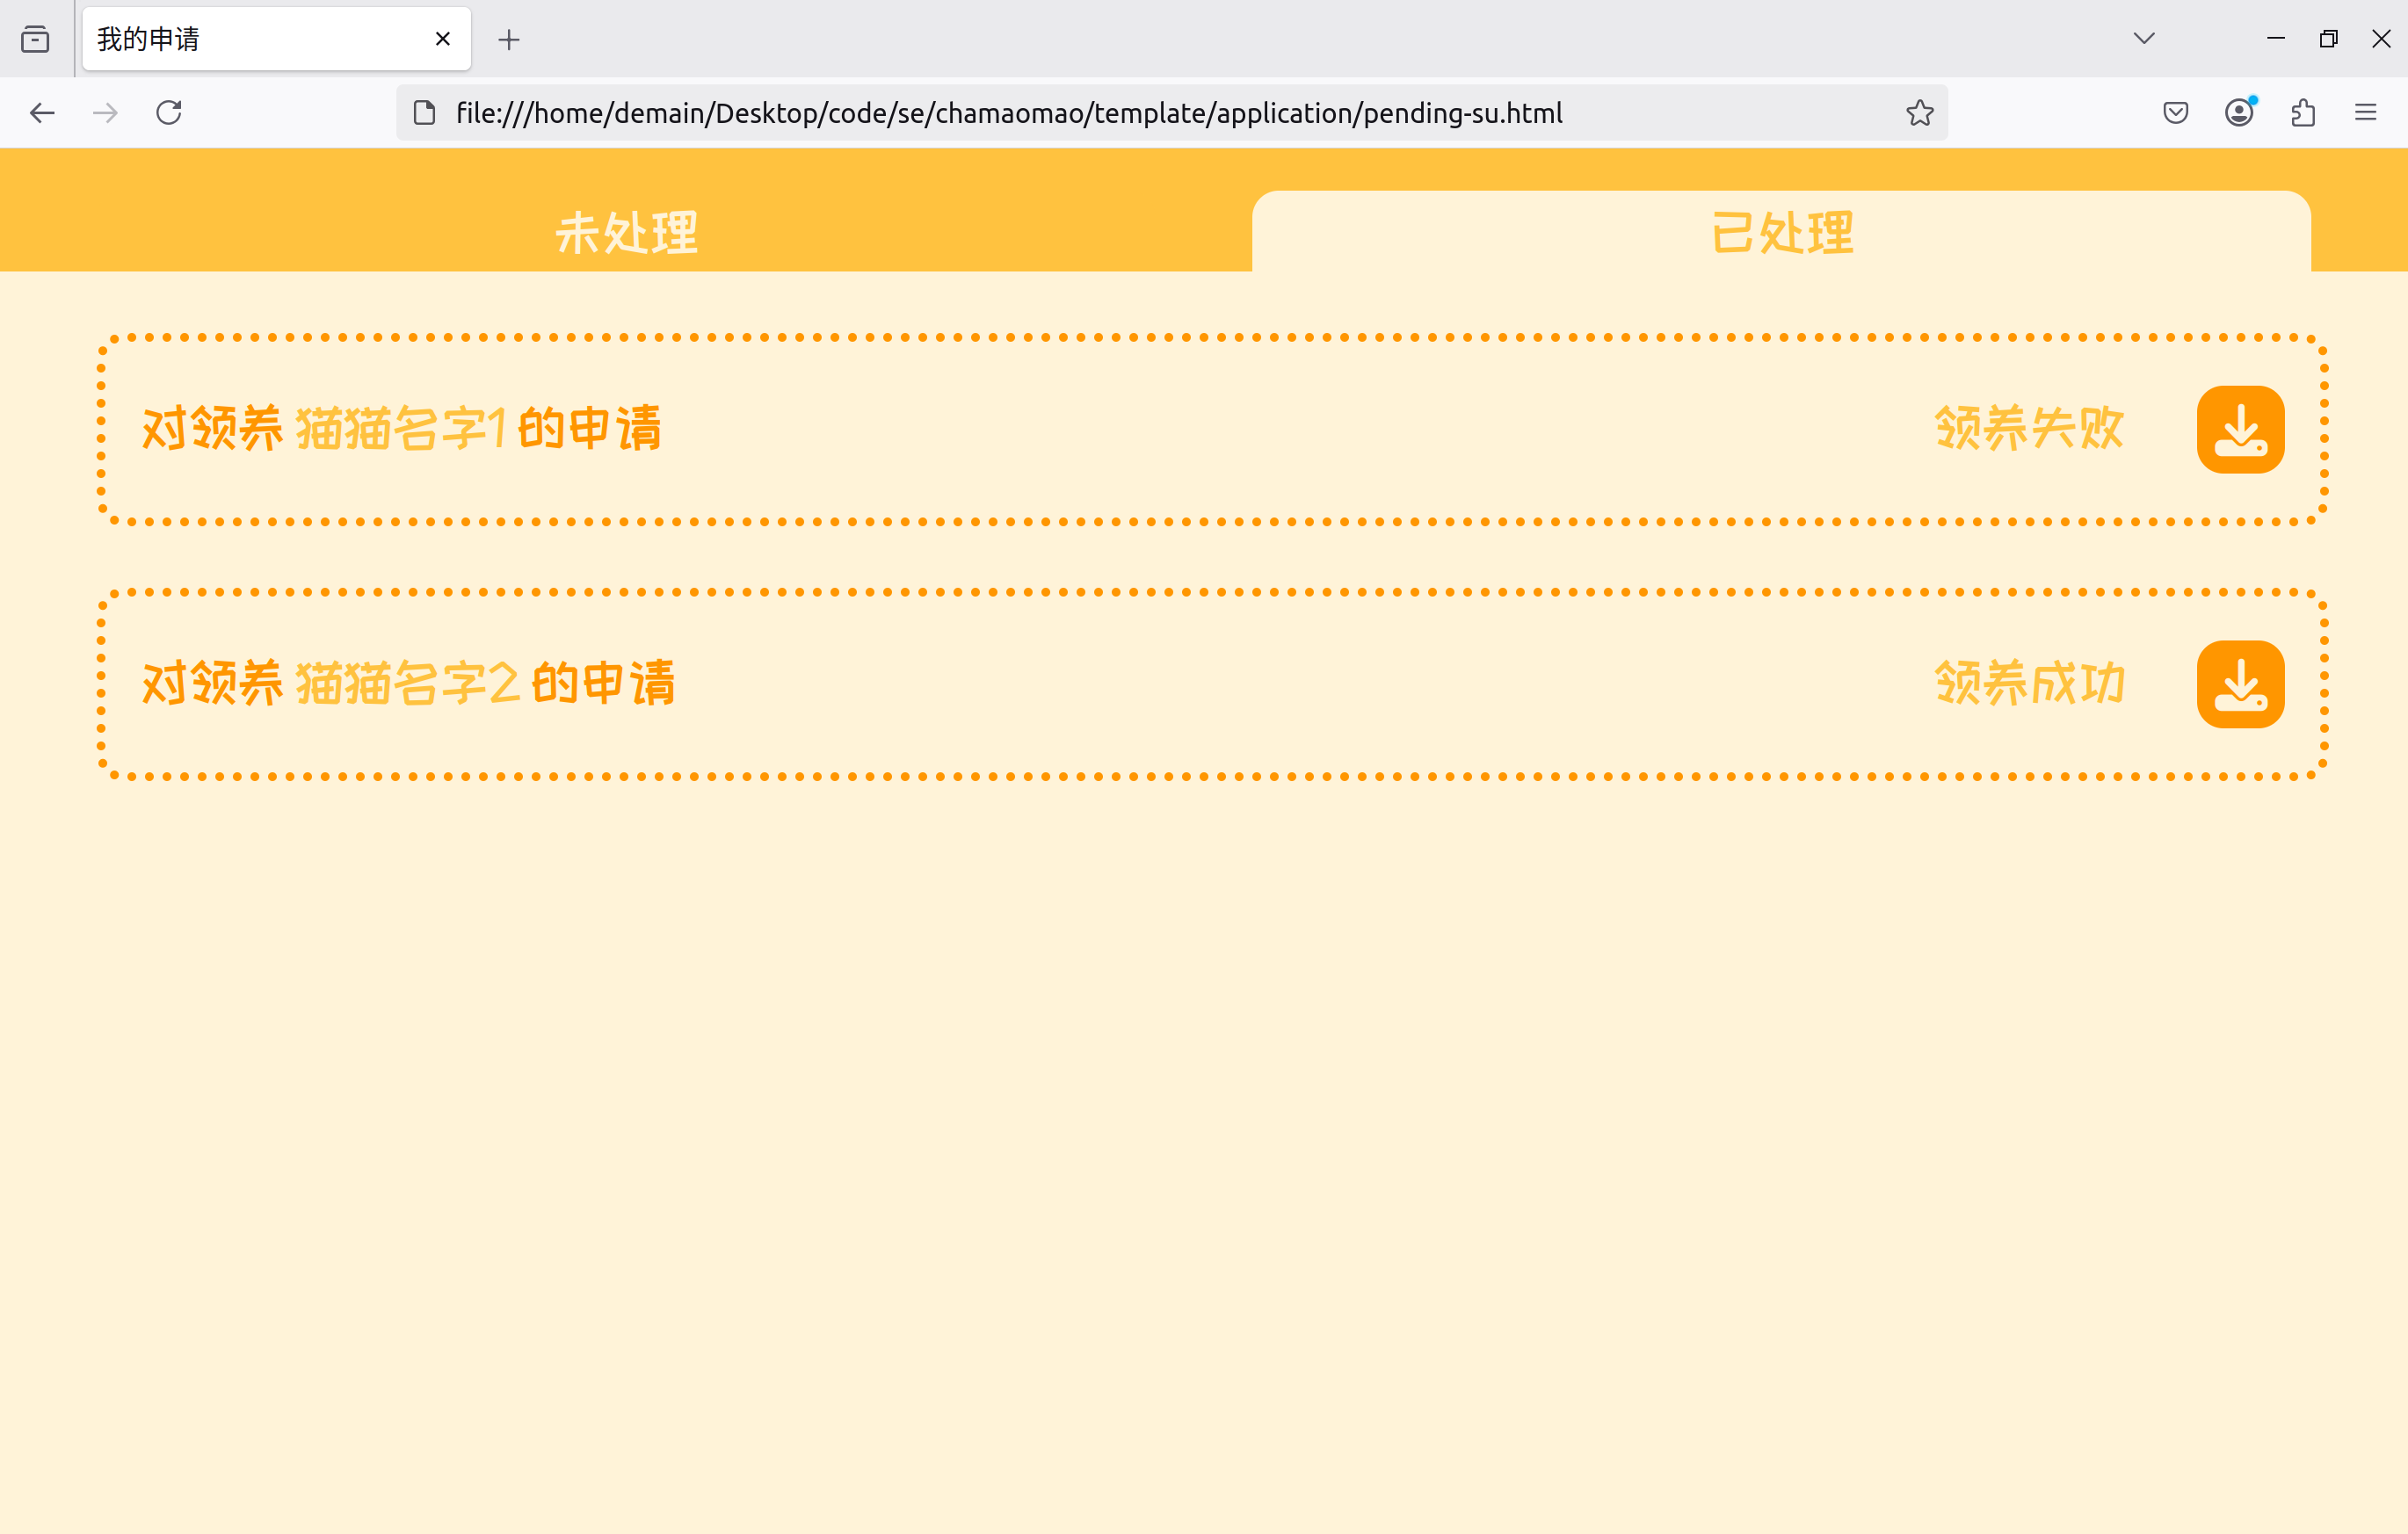
\includegraphics[width=0.9\textwidth]{figures/AdoptionApply4.png}
\end{figure}

\subsubsection{动物地图管理界面}

\begin{figure}[H]
  \centering
  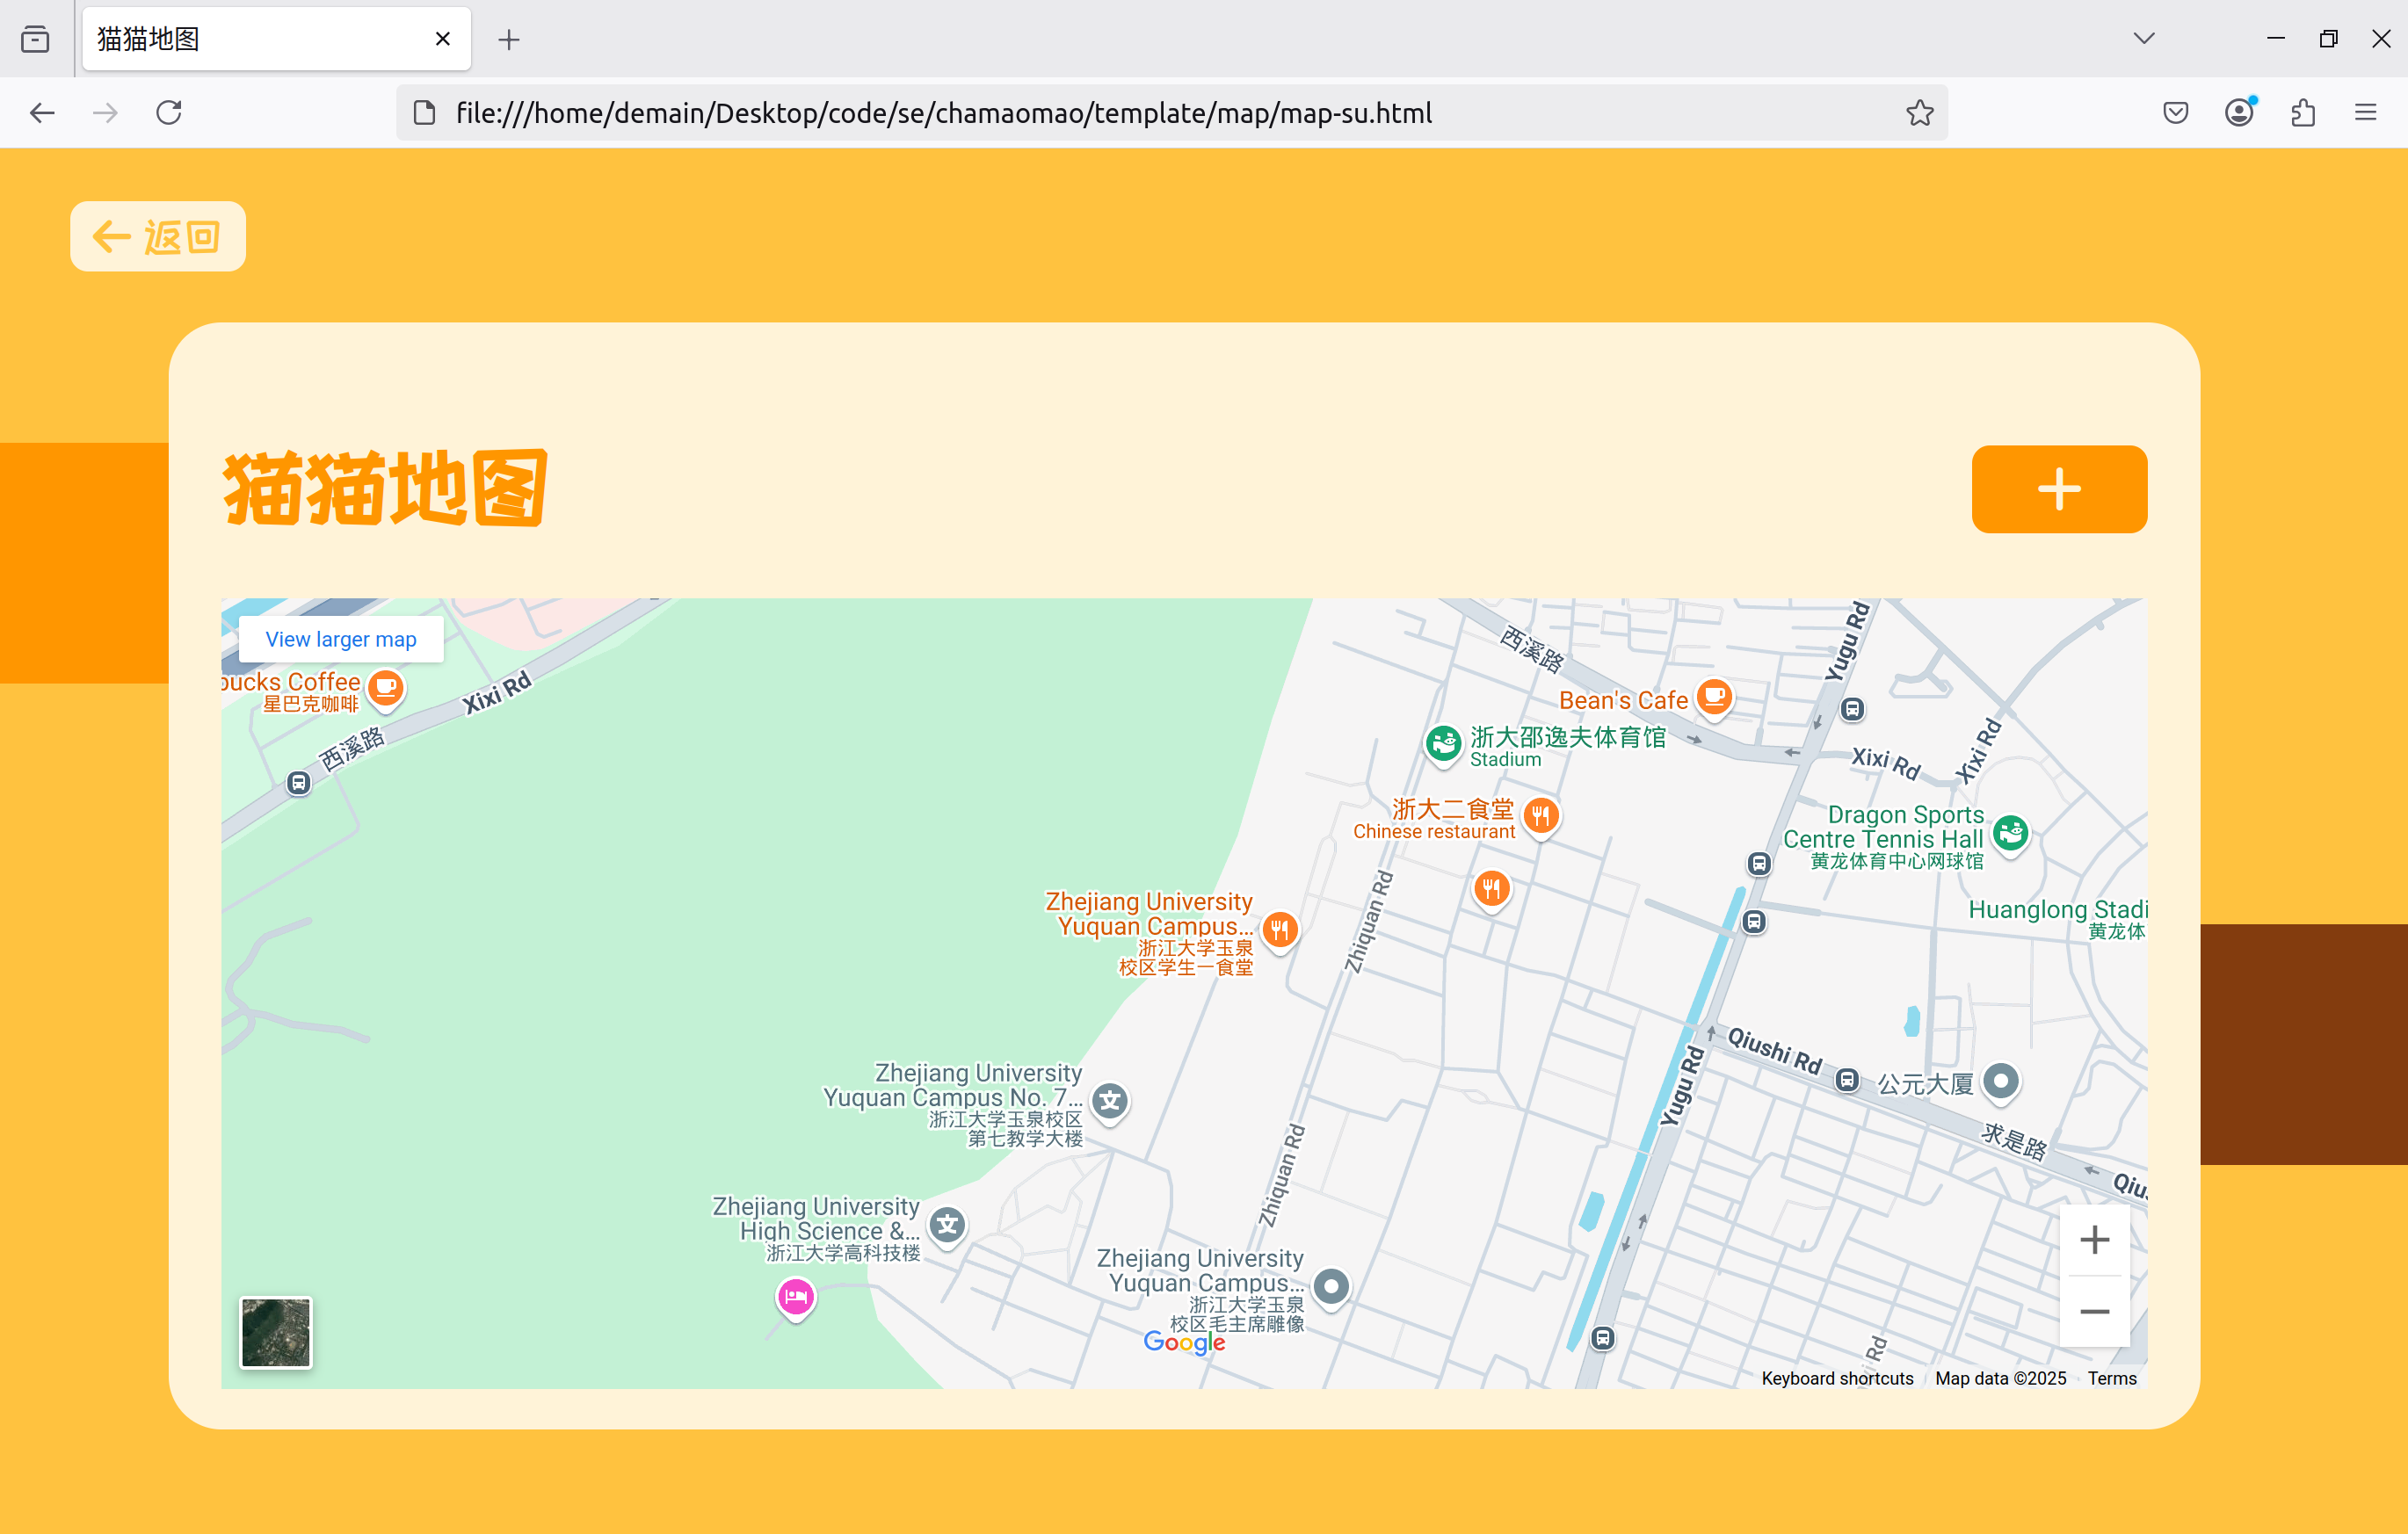
\includegraphics[width=0.9\textwidth]{figures/AdministratorMap.png}
\end{figure}

\subsubsection{领养指南管理界面}

\begin{figure}[H]
  \centering
  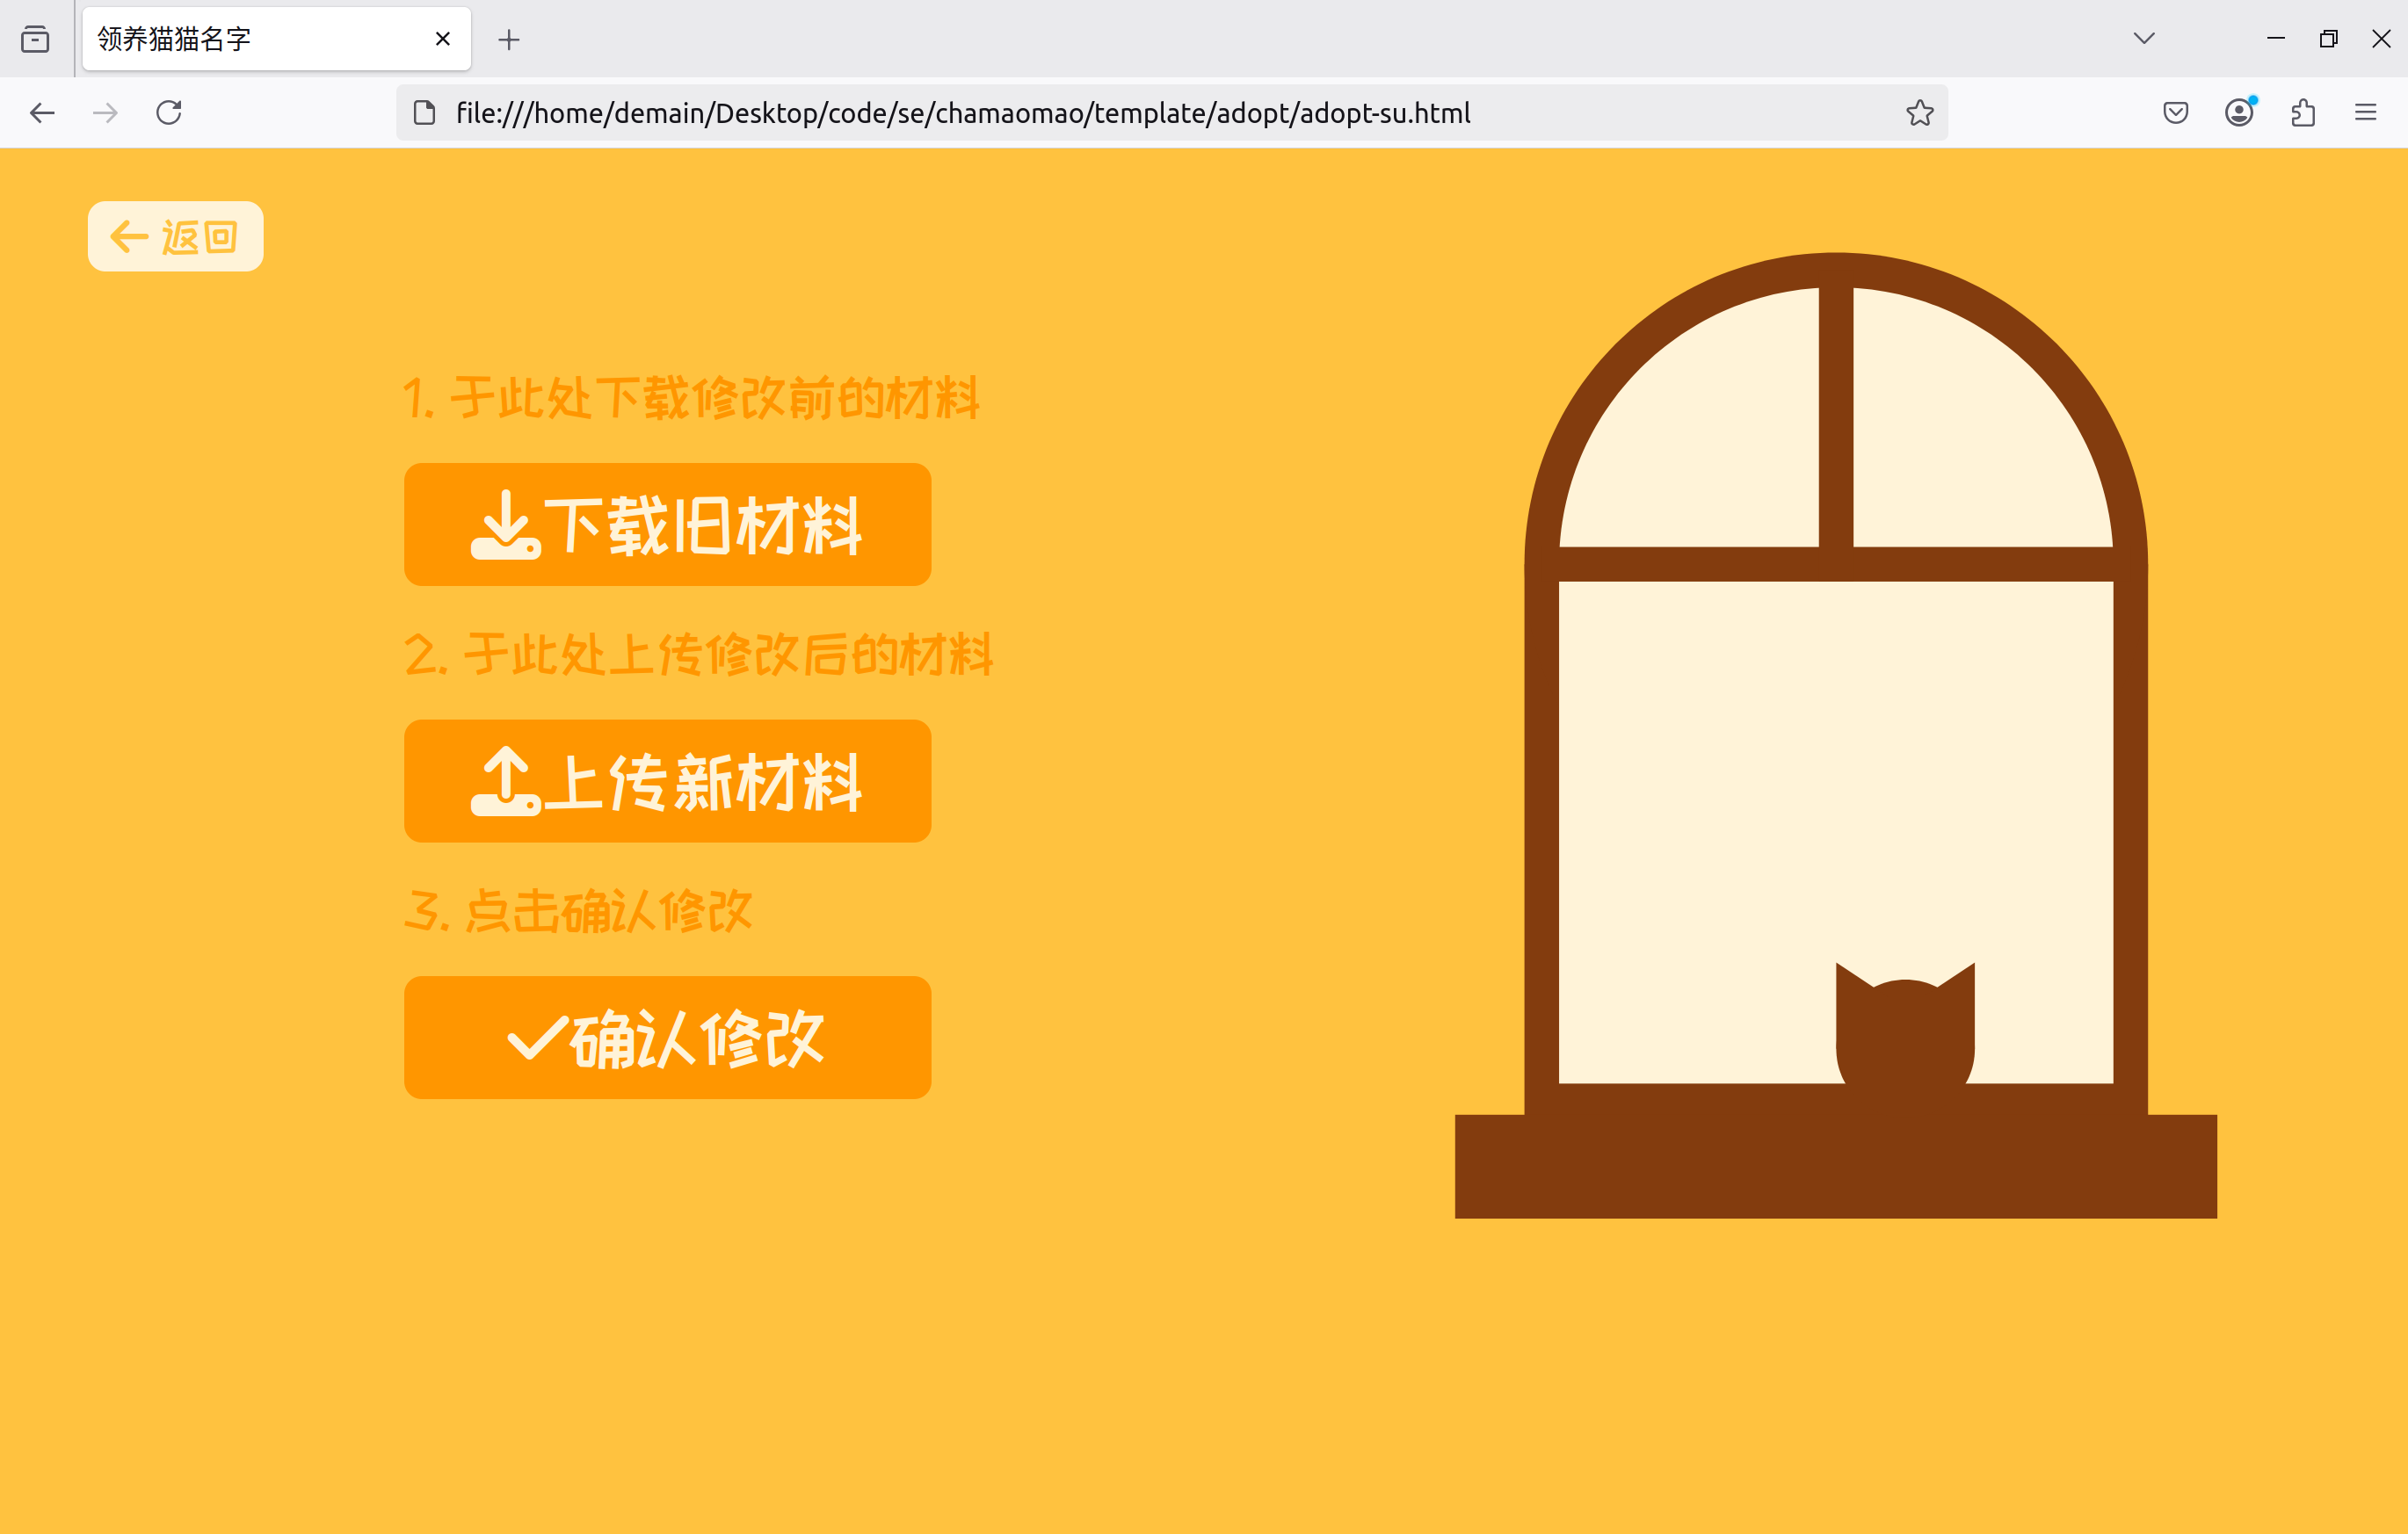
\includegraphics[width=0.9\textwidth]{figures/Guide.png}
\end{figure}

\section{详细设计} \label{a}

本章主要介绍项目前端、后端、以及前后端间定义的各种接口 

\subsection{前端内部接口}

主要涉及 \verb|Vue| 文件中 \verb|script| 块的 \verb|methods| 部分定义的函数

\subsubsection{基础信息模块}

\begin{itemize}

  \item \verb|Validate|
  \begin{itemize}
  \item \textbf{接口描述:}用于校验输入账号或密码的格式是否正确
  \item \textbf{实现思路:}包括非法字符的识别、长度检测等过程
  \end{itemize}

  \item \verb|LoginRequest|
  \begin{itemize}
  \item \textbf{接口描述:}处理登录请求,如果格式不符或者密码错误,给出提示;登陆成功后跳转到系统首页
  \item \textbf{实现思路:}先调用 \verb|Validate| 接口校验账号密码格式,校验通过后进行加密,再向后端发送 \verb|POST| 请求;根据后端传回的信息,判断是否登录成功;登陆成功后,判断是普通用户还是管理员,跳转到对应首页
  \end{itemize}

  \item \verb|RegisterRequest|
  \begin{itemize}
  \item \textbf{接口描述:}处理注册请求,如果格式不符,给出提示;注册成功后跳转回登录界面
  \item \textbf{实现思路:}先调用 \verb|Validate| 接口校验密码格式,校验通过后进行加密,再向后端发送 \verb|POST| 请求;根据后端传回的信息,判断是否注册成功;注册成功后,跳转回登录界面
  \end{itemize}

  \item \verb|PersonalInfoQuery|
  \begin{itemize}
  \item \textbf{接口描述:}获取个人信息用于显示
  \item \textbf{实现思路:}向后端发送 \verb|GET| 请求;根据后端传回的数据,将个人信息存到 \verb|PersonalInfo| 结构体中
  \end{itemize}

  \item \verb|ConfirmPersonalInfoModify|
  \begin{itemize}
  \item \textbf{接口描述:}将修改后的个人信息同步到后端数据库,如果修改成功,给出提示
  \item \textbf{实现思路:}向后端发送 \verb|POST| 请求,传递 \verb|PersonalInfo| 结构体;根据后端传回的信息,判断是否修改成功,进行相应显示
  \end{itemize}

  \item \verb|QueryUsers|
  \begin{itemize}
  \item \textbf{接口描述:}供管理员查询所有普通用户的个人信息,显示在用户管理界面
  \item \textbf{实现思路:}向后端发送 \verb|GET| 请求;得到响应后,将 \verb|this.users| 清空,创建一个临时变量 \verb|users| 来获取响应负载,将其中的每个元素加到 \verb|this.users| 中,页面更新后便会进行显示。
  \end{itemize}

  \item \verb|QueryAnimals|
  \begin{itemize}
  \item \textbf{接口描述:}供用户查询动物详细信息
  \item \textbf{实现思路:}向后端发送 \verb|POST| 请求,传递 \verb|ToQuery| 结构体,内部包含动物品种、姓名等查询条件;得到响应后,将 \verb|this.animals| 清空,创建一个临时变量 \verb|animals| 来获取响应负载,将其中的每个元素加到 \verb|this.animals| 中,页面更新后便会进行显示。
  \end{itemize}

  \item \verb|ImageFileValidate|
  \begin{itemize}
  \item \textbf{接口描述:}图片上传前,检查类型和大小等
  \item \textbf{实现思路:}自定义要求进行检查,检查通过后,保存在 \verb|ImageFile| 对象中,暂时位于浏览器内存中,后续可以用于构造 \verb|AnimalInfo| 对象,发往后端
  \end{itemize}

  \item \verb|AnimalInfoUpload|
  \begin{itemize}
  \item \textbf{接口描述:}新建动物,上传动物信息,待管理员审核通过后再加入数据库
  \item \textbf{实现思路:}向后端发送 \verb|POST| 请求,传递 \verb|AnimalInfo| 结构体;根据后端传回的信息,判断是否上传成功,进行相应显示
  \end{itemize}

  \item \verb|AnimalInfoModify|
  \begin{itemize}
  \item \textbf{接口描述:}管理员修改动物信息
  \item \textbf{实现思路:}向后端发送 \verb|POST| 请求,传递 \verb|AnimalInfo| 结构体;根据后端传回的信息,判断是否修改成功,进行相应显示
  \end{itemize}

  \item \verb|AnimalInfoDelete|
  \begin{itemize}
  \item \textbf{接口描述:}管理员删除动物信息
  \item \textbf{实现思路:}向后端发送 \verb|DELETE| 请求,指明动物 \verb|id|;根据后端传回的信息,判断是否删除成功,进行相应显示
  \end{itemize}

\end{itemize}

\subsubsection{动物领养申请模块}

\begin{itemize}

  \item \verb|FormDownload|
  \begin{itemize}
  \item \textbf{接口描述:}用户下载领养申请表
  \item \textbf{实现思路:}向后端发送 \verb|GET| 请求,端口号为领养申请表文件服务器对应的端口号
  \end{itemize}

  \item \verb|FormUpload|
  \begin{itemize}
  \item \textbf{接口描述:}点击“提交申请”按钮后,用户上传填好的领养申请表
  \item \textbf{实现思路:}向后端发送 \verb|POST| 请求,端口号为领养申请表文件服务器对应的端口号,传递 \verb|FormData| 结构体;根据后端传回的信息,判断是否上传成功
  \end{itemize}

  \item \verb|AdoptionApply|
  \begin{itemize}
  \item \textbf{接口描述:}添加一条领养申请
  \item \textbf{实现思路:}向后端发送 \verb|POST| 请求,传递 \verb|AdoptionApplyInfo| 结构体
  \end{itemize}

  \item \verb|QueryAdoptionApply|
  \begin{itemize}
  \item \textbf{接口描述:}查询领养记录
  \item \textbf{实现思路:}向后端发送 \verb|GET| 请求,附带参数,表明是用户还是管理员的请求;得到响应后,将 \verb|this.adoptions| 清空,创建一个临时变量 \verb|adoptions| 来获取响应负载,将其中的每个元素加到 \verb|this.adoptions| 中,页面更新后便会进行显示。
  \end{itemize}
  
  \item \verb|ReviewAdoptionApply|
  \begin{itemize}
  \item \textbf{接口描述:}管理员审核用户的领养申请
  \item \textbf{实现思路:}向后端发送 \verb|POST| 请求,传递 \verb|ReviewOpinion| 结构体,后端可以据此修改数据库中的审核记录
  \end{itemize}

  \item \verb|AdoptionPost|
  \begin{itemize}
  \item \textbf{接口描述:}管理员发布领养信息,同步到数据库中
  \item \textbf{实现思路:}向后端发送 \verb|POST| 请求,传递 \verb|AdoptionPostInfo| 结构体;根据后端传回的信息,判断是否发布成功
  \end{itemize}

  \item \verb|QueryAdoptionPost|
  \begin{itemize}
  \item \textbf{接口描述:}查询所有已发布的领养信息,供用户挑选
  \item \textbf{实现思路:}向后端发送 \verb|GET| 请求;得到响应后,将 \verb|this.adoptions| 清空,创建一个临时变量 \verb|adoptions| 来获取响应负载,将其中的每个元素加到 \verb|this.adoptions| 中,页面更新后便会进行显示。
  \end{itemize}

  \item \verb|DeleteAdoptionPost|
  \begin{itemize}
  \item \textbf{接口描述:}管理员删除领养信息,同步到数据库中
  \item \textbf{实现思路:}向后端发送 \verb|DELETE| 请求,传递参数 \verb|adoption_post_id|;根据后端传回的信息,判断是否删除成功
  \end{itemize}

  \item \verb|GuideDownload|
  \begin{itemize}
  \item \textbf{接口描述:}下载领养指南
  \item \textbf{实现思路:}向后端发送 \verb|GET| 请求,端口号为领养指南文件服务器对应的端口号
  \end{itemize}

  \item \verb|GuideUpload|
  \begin{itemize}
  \item \textbf{接口描述:}点击“确认修改”按钮后,上传修改好的领养指南
  \item \textbf{实现思路:}向后端发送 \verb|POST| 请求,端口号为领养指南文件服务器对应的端口号,传递 \verb|GuideData| 结构体;根据后端传回的信息,判断是否上传成功
  \end{itemize}

\end{itemize}

\subsubsection{动物地图模块}

\begin{itemize}

  \item \verb|MapShow|
  \begin{itemize}
  \item \textbf{接口描述:}显示动物地图
  \item \textbf{实现思路:}主要利用  \verb|AMapLoader| 库调用高德地图提供的 \verb|API| 实现。先使用申请好的 \verb|Web| 端开发者 \verb|Key|,调用  \verb|AMapLoader.load()| 方法载入地图;再设置好显示范围、地图中心点;然后向后端发送 \verb|GET| 请求查询所有动物的位置信息进行缓存;根据位置信息为每个动物创建 \verb|Marker| 对象,并将它们添加到地图中形成标记
  \end{itemize}

\end{itemize}

\subsection{前后端间交互接口}

这些接口主要由后端提供,解析来自前端的请求,分配路由,然后查询数据库、返回数据等。在本系统中,我们采用 \verb|REST| 风格的 \verb|API| 制定模式。

\subsubsection{axios库}

\verb|axios| 是一个基于 \verb|promise| 的网络请求库,为前端提供与后端交互的接口。本项目中我们通过 \verb|axios| 向后端发送网络请求并接收响应,其中主要使用 \verb|GET| 和 \verb|POST| 方法

\subsubsection{HttpHandler接口}

在 \verb|Java| 中,\verb|HttpHandler| 类是一个接口,它定义了处理 \verb|HTTP| 请求的方法。本项目中,我们通过重写其中的 \verb|handle| 方法,来重新实现这一接口,从而处理不同的 \verb|HTTP| 请求。

具体而言,我们根据 \verb|URL| 路径的不同,创建不同的类来实现 \verb|HttpHandler| 接口;然后在 \verb|handle| 方法中,根据请求类型,会调用 \verb|handleGetRequest()|、\verb|handlePostRequest()| 这两个方法,因此我们也需要重写这两个方法,处理对应请求

下面按类进行接口的介绍

\begin{itemize}

  \item \verb|LoginHandler|
  \begin{itemize}
  \item \textbf{接口描述:}处理前端发来的登录的 \verb|POST| 请求
  \item \textbf{实现思路:}调用后端提供的 \verb|QueryUser| 接口,在用户表中对账号和密码字段进行精确查找,如果找到,向前端发送登陆成功的信息,反之发送登录失败的信息
  \end{itemize}

  \item \verb|RegisterHandler|
  \begin{itemize}
  \item \textbf{接口描述:}处理前端发来的注册的 \verb|POST| 请求
  \item \textbf{实现思路:}调用后端提供的 \verb|RegisterUser| 接口,在用户表中添加一条记录,向前端发送注册成功的信息;其中,\verb|users_id| 作为自增列,插入时由数据库生成,插入完成后,会一同返回给前端
  \end{itemize}

  \item \verb|PersonalInfoHandler|
  \begin{itemize}
  \item \textbf{接口描述:}处理前端发来的个人信息的 \verb|GET| 和 \verb|POST| 请求
  \item \textbf{handleGetRequest()实现思路:}调用后端提供的 \verb|QueryUser| 接口,根据 \verb|GET| 请求的参数(\verb|users_id|),在用户表中进行精确查找,如果找到,向前端发送对应用户数据,反之报错
  \item \textbf{handlePostRequest()实现思路:}调用后端提供的 \verb|ModifyUser| 接口,根据 \verb|POST| 请求的参数(\verb|PersonalInfo|),在用户表中进行更新,并向前端汇报
  \end{itemize}

  \item \verb|UsersInfoHandler|
  \begin{itemize}
  \item \textbf{接口描述:}处理前端发来的所有用户信息的 \verb|GET| 请求
  \item \textbf{实现思路:}调用后端提供的 \verb|QueryUser| 接口,查询条件为空,查询成功后发往前端
  \end{itemize}

  \item \verb|AnimalInfoHandler|
  \begin{itemize}
  \item \textbf{接口描述:}处理前端发来的动物信息的 \verb|GET|、 \verb|POST|、 \verb|PUT| 请求
  \item \textbf{handleGetRequest()实现思路:}调用后端提供的 \verb|QueryAnimal| 接口,根据 \verb|GET| 请求的参数,在动物表中进行查找,向前端发送查询结果
  \item \textbf{handlePostRequest()实现思路:}调用后端提供的 \verb|AddAnimal| 接口,根据 \verb|POST| 请求的参数,在动物表中添加一条记录,向前端发送注册成功的信息;其中,\verb|animal_id| 作为自增列,插入时由数据库生成,插入完成后,会一同返回给前端
  \item \textbf{handlePutRequest()实现思路:}调用后端提供的 \verb|ModifyAnimal| 接口,根据 \verb|PUT| 请求的参数,在动物表中进行更新,并向前端汇报
  \item \textbf{handleDeleteRequest()实现思路:}调用后端提供的 \verb|DeleteAnimal| 接口,根据 \verb|DELETE| 请求的参数,在动物表中进行删除,并向前端汇报
  \end{itemize}

  \item \verb|AdoptionApplyHandler|
  \begin{itemize}
  \item \textbf{接口描述:}处理前端发来的领养记录的 \verb|GET|、 \verb|POST|、 \verb|PUT| 请求
  \item \textbf{handleGetRequest()实现思路:}调用后端提供的 \verb|QueryAdoptionApply| 接口,根据 \verb|GET| 请求的参数,判断是返回所有记录,还是指定用户的记录
  \item \textbf{handlePostRequest()实现思路:}调用后端提供的 \verb|AddAdoptionApply| 接口,根据 \verb|POST| 请求的参数,在领养申请表中添加领养申请记录,将申请结果返回前端
  \item \textbf{handlePutRequest()实现思路:}调用后端提供的 \verb|ModifyAdoptionApply| 接口,根据 \verb|PUT| 请求的参数,对指定领养记录的“申请状态”与“审核意见”进行修改;如果审核通过,再调用后端提供的 \verb|ModifyAnimal| 接口,修改该动物的信息表明其已经被领养
  \end{itemize}

  \item \verb|AdoptionPostHandler|
  \begin{itemize}
  \item \textbf{接口描述:}处理前端发来的待领养信息的 \verb|GET|、 \verb|POST| 请求
  \item \textbf{handleGetRequest()实现思路:}调用后端提供的 \verb|QueryAdoptionPost| 接口,返回所有待领养信息
  \item \textbf{handlePostRequest()实现思路:}调用后端提供的 \verb|AddAdoptionPost| 接口,根据 \verb|POST| 请求的参数,在待领养表中添加记录
  \item \textbf{handleDeleteRequest()实现思路:}调用后端提供的 \verb|DeleteAdoptionPost| 接口,根据 \verb|DELETE| 请求的参数,在待领养表中进行删除,并向前端汇报
  \end{itemize}

  \item \verb|AdoptionGuideHandler|
  \begin{itemize}
  \item \textbf{接口描述:}处理前端发来的领养指南的 \verb|GET| 请求
  \item \textbf{handleGetRequest()实现思路:}调用后端提供的 \verb|QueryAdoptionGuide| 接口,查询所有已发布的领养指南,返回给前端
  \item \textbf{handlePostRequest()实现思路:}调用后端提供的 \verb|AddAdoptionGuide| 接口,根据 \verb|POST| 请求的参数,在领养指南表中添加记录
  \end{itemize}

\end{itemize}

\subsubsection{Express依赖}

这里利用 \verb|Node.js| 及其常用的 \verb|Web| 框架 \verb|Express|,实现文件上传和下载的功能

\begin{itemize}

  \item \verb|post|
  \begin{itemize}
  \item \textbf{接口描述:}处理前端发来的 \verb|POST| 请求
  \item \textbf{实现思路:}首先指定好本地存储位置,定义 \verb|multer| 中间件,再使用中间件实现文件的保存
  \end{itemize}

  \item \verb|get|
  \begin{itemize}
  \item \textbf{接口描述:}处理前端发来的 \verb|GET| 请求
  \item \textbf{实现思路:}根据提前规定好的文件路径,构造完整文件路径,直接调用 \verb|res.download(filepath)| 方法即可,会自动将文件发送到浏览器并弹出下载框
  \end{itemize}

\end{itemize}

\subsection{后端内部接口}

主要涉及针对不同数据库的各种操作

\subsubsection{基础信息模块}

\begin{itemize}

  \item \verb|QueryUser|
  \begin{itemize}
  \item \textbf{接口描述:}根据提供的查询条件查询符合条件的用户,并按照指定排序方式排序。
  \item \textbf{实现思路:}根据查询条件构造 \verb|SELECT| 语句在用户信息数据库中查询即可
  \end{itemize}

  \item \verb|RegisterUser|
  \begin{itemize}
  \item \textbf{接口描述:}根据提供的用户个人信息(主要是账号密码),完成新用户注册。
  \item \textbf{实现思路:}构造 \verb|INSERT| 语句在用户表中插入一条记录
  \end{itemize}

  \item \verb|ModifyUser|
  \begin{itemize}
  \item \textbf{接口描述:}根据提供的新的用户个人信息,完成数据库中个人信息的修改。
  \item \textbf{实现思路:}构造 \verb|UPDATE| 语句在用户表中更新
  \end{itemize}

  \item \verb|AddAnimal|
  \begin{itemize}
  \item \textbf{接口描述:}根据提供的新的动物信息,完成数据库中动物信息的添加。
  \item \textbf{实现思路:}构造 \verb|INSERT| 语句在动物表中插入一条记录
  \end{itemize}

  \item \verb|QueryAnimal|
  \begin{itemize}
  \item \textbf{接口描述:}根据提供的查询条件查询符合条件的动物,并按照指定排序方式排序。
  \item \textbf{实现思路:}根据查询条件构造 \verb|SELECT| 语句在动物信息数据库中查询即可
  \end{itemize}

  \item \verb|ModifyAnimal|
  \begin{itemize}
  \item \textbf{接口描述:}根据提供的新的动物信息,完成数据库中动物信息的修改。
  \item \textbf{实现思路:}构造 \verb|UPDATE| 语句在动物表中更新
  \end{itemize}

  \item \verb|DeleteAnimal|
  \begin{itemize}
  \item \textbf{接口描述:}根据提供的\verb|aninmal_id|,完成数据库中动物信息的删除。
  \item \textbf{实现思路:}首先构造 \verb|SELECT| 语句在动物表中查询,如果要删除的动物不存在,那么提示删除失败;构造 \verb|DELETE| 语句在动物表中进行删除
  \end{itemize}

\end{itemize}

\subsubsection{动物领养模块}

\begin{itemize}

  \item \verb|QueryAdoptionApply|
  \begin{itemize}
  \item \textbf{接口描述:}根据提供的查询条件查询符合条件的领养记录,并按照指定排序方式排序。
  \item \textbf{实现思路:}根据查询条件构造 \verb|SELECT| 语句在领养申请表中查询即可
  \end{itemize}

  \item \verb|ModifyAdoptionApply|
  \begin{itemize}
  \item \textbf{接口描述:}根据提供的审核意见 \verb|ReviewOpinion|,完成数据库中领养申请记录的修改。
  \item \textbf{实现思路:}构造 \verb|UPDATE| 语句在领养申请表中更新
  \end{itemize}

  \item \verb|AddAdoptionApply|
  \begin{itemize}
  \item \textbf{接口描述:}根据提供的新的领养信息,完成数据库中领养申请记录的添加。
  \item \textbf{实现思路:}首先构造 \verb|SELECT| 语句在领养申请表中查询,如果该用户对相同动物的领养记录已经存在,那么添加失败;构造 \verb|INSERT| 语句在动物表中插入一条记录
  \end{itemize}

  \item \verb|QueryAdoptionPost|
  \begin{itemize}
  \item \textbf{接口描述:}根据提供的查询条件查询符合条件的待领养信息,并按照指定排序方式排序。
  \item \textbf{实现思路:}根据查询条件构造 \verb|SELECT| 语句在待领养信息表中查询即可
  \end{itemize}

  \item \verb|AddAdoptionPost|
  \begin{itemize}
  \item \textbf{接口描述:}根据提供的新的待领养信息,完成数据库中待领养记录的添加。
  \item \textbf{实现思路:}首先构造 \verb|SELECT| 语句在待领养信息表中查询,如果相同动物的待领养信息已经存在,那么添加失败;构造 \verb|INSERT| 语句在待领养信息表中插入一条记录
  \end{itemize}

  \item \verb|DeleteAdoptionPost|
  \begin{itemize}
  \item \textbf{接口描述:}根据提供的\verb|adoption_post_id|,完成数据库中待领养信息的删除。
  \item \textbf{实现思路:}首先构造 \verb|SELECT| 语句在待领养表中查询,如果要删除的动物不存在,那么提示删除失败;构造 \verb|DELETE| 语句在待领养表中进行删除
  \end{itemize}

\end{itemize}

\section{可靠性及安全性设计}

\subsection{系统可靠性设计}

\subsubsection{数据持久化与一致性保障}

\noindent\textbf{数据库选择与配置}

选用成熟稳定的关系型数据库管理系统,如本系统使用的 \verb|MySQL|,并进行合理的配置和优化。

\vspace{0.25cm}

\noindent\textbf{事务管理}

对于涉及多个数据表更新的关键业务操作,须采用数据库事务来确保操作的原子性。如果系列操作中任何一步失败,所有已执行的操作都将回滚,从而避免数据不一致状态。

\vspace{0.25cm}

\noindent\textbf{数据校验}

在数据写入数据库之前进行严格的数据校验(类型、格式、范围、业务规则),防止非法或无效数据污染数据库。

\subsubsection{容错与故障恢复设计}

\noindent\textbf{错误处理机制}

系统各模块应包含健壮的错误处理逻辑。对于可预见的错误(如用户输入错误、资源未找到),应向用户返回清晰的提示信息。

对于不可预见的内部错误或异常,系统应能捕获并记录详细的错误日志,同时避免将敏感的系统内部错误信息直接暴露给用户,而是显示通用的错误提示。

\vspace{0.25cm}

\noindent\textbf{数据备份与恢复}

必须制定并严格执行数据库的定期备份策略,备份数据应存储在与生产数据库物理隔离的安全位置。

\subsubsection{系统监控与日志记录}

\noindent\textbf{应用性能监控}

在可行的条件下,可以部署应用性能监控工具,实时监控服务器的关键性能指标

\vspace{0.25cm}

\noindent\textbf{全面的日志记录}

记录详细的应用运行日志、错误日志、用户操作日志和安全审计日志。日志应包含时间戳、事件级别、来源、详细信息等,便于问题排查、性能分析和安全审计。


\subsection{系统安全性设计}

\subsubsection{身份认证与授权}

\noindent\textbf{强密码策略与存储}

严禁明文存储用户密码,且制用户设置符合一定复杂度要求的密码。

\vspace{0.25cm}

\noindent\textbf{会话管理}

使用随机且足够长度的会话 \verb|ID|,提供安全的登出机制,确保服务器端和客户端会话均被有效终止。

\vspace{0.25cm}

\noindent\textbf{基于角色的访问控制}

严格区分普通用户和管理员的角色。

每个角色拥有明确定义的权限集合,权限应遵循最小权限原则,即仅授予完成其任务所必需的最小权限。

后端 \verb|API| 接口必须对每个请求进行严格的身份认证和权限校验,确保用户只能访问其被授权的资源和操作。

\subsubsection{数据传输安全}

涉及敏感数据的传输必须使用安全的传输协议,如 \verb|HTTPS|,以防止中间人攻击和数据泄露。

\subsubsection{输入验证}

对所有来自用户端或外部系统的输入数据,在服务器端进行严格的合法性校验,包括数据类型、格式、长度、取值范围以及特殊字符的过滤或转义。


严禁直接拼接 \verb|SQL| 语句,避免将用户输入直接作为命令或参数传递给服务端系统执行。

\subsubsection{安全审计与日志}

记录所有与安全相关的事件,包括用户登录、登出、权限变更、敏感数据访问等。

安全日志应受到严格保护,防止未授权的访问和篡改,并定期进行审查。

\subsection{系统出错设计}

\subsubsection{错误信息分类与提示}

\noindent\textbf{用户操作错误}

如表单填写不符合规范、输入数据格式错误等。

处理方法:前端进行即时校验并给出明确、友好的错误提示,引导用户修正。

\vspace{0.25cm}

\noindent\textbf{业务逻辑错误}

如申请领养已被领养的动物、用户权限不足等。

处理方法:后端进行业务逻辑校验,返回明确的错误信息,前端展示给用户。

\vspace{0.25cm}

\noindent\textbf{资源未找到}

如访问一个不存在的动物详情页或用户页面。

处理方法:返回标准的 \verb|404 Not Found| 页面,并提供导航回主页的选项。

\vspace{0.25cm}

\noindent\textbf{服务器内部错误}

如数据库连接失败、代码缺陷导致的运行时异常等。

处理方法:系统应捕获此类异常,记录详细的错误日志;向用户显示一个通用的、不暴露内部细节的错误页面或提示;将错误信息发送给管理员进行后续处理。

\vspace{0.25cm}

\noindent\textbf{网络连接问题}

处理方法:客户端应能检测到网络中断,并提示用户检查网络连接。对于需要网络请求的操作,在请求失败时给出相应提示。

\subsection{补救措施}

进行数据恢复,通过定期备份和验证的恢复计划,确保在数据损坏或丢失时能够将数据恢复到最近的一致状态。

将系统重启和恢复服务,通过详细的日志定位和解决问题。

\subsection{系统维护设计}

清晰的文档:完备的需求文档、设计文档、\verb|API| 文档、运行使用手册,便于快速理解系统和定位问题。

模块化设计:高内聚、低耦合的模块划分,更容易隔离和修复故障。

规范的编码与注释:清晰、可读的代码和必要的注释,有助于开发和维护人员快速理解代码逻辑。

同时,系统维护人员及时更新技术漏洞,通过各种手段防止各种对系统的攻击,增加代码
的可靠性。也需要定期维护数据库,包括检查数据库表与日志文件等,确保数据库内数据的正确性。

\end{document}
